\documentclass[compress]{beamer}
\usepackage{ifthen,verbatim}

\newcommand{\isnote}{}
\xdefinecolor{lightyellow}{rgb}{1.,1.,0.25}
\xdefinecolor{darkblue}{rgb}{0.1,0.1,0.7}

%% Uncomment this to get annotations
%% \def\notes{\addtocounter{page}{-1}
%%            \renewcommand{\isnote}{*}
%% 	   \beamertemplateshadingbackground{lightyellow}{white}
%%            \begin{frame}
%%            \frametitle{Notes for the previous page (page \insertpagenumber)}
%%            \itemize}
%% \def\endnotes{\enditemize
%% 	      \end{frame}
%%               \beamertemplateshadingbackground{white}{white}
%%               \renewcommand{\isnote}{}}

%% Uncomment this to not get annotations
\def\notes{\comment}
\def\endnotes{\endcomment}

\setbeamertemplate{navigation symbols}{}
\setbeamertemplate{headline}{\mbox{ } \hfill
\begin{minipage}{5.5 cm}
\vspace{-0.75 cm} \small
\end{minipage} \hfill
\begin{minipage}{4.5 cm}
\vspace{-0.75 cm} \small
\begin{flushright}
\ifthenelse{\equal{\insertpagenumber}{1}}{}{Jim Pivarski \hspace{0.2 cm} \insertpagenumber\isnote/\pageref{numpages}}
\end{flushright}
\end{minipage}\mbox{\hspace{0.2 cm}}\includegraphics[height=1 cm]{../cmslogo} \hspace{0.1 cm} \includegraphics[height=1 cm]{../tamulogo} \hspace{0.01 cm} \vspace{-1.05 cm}}

\begin{document}
\begin{frame}
\vfill
\begin{center}
\textcolor{darkblue}{\Large Updates in CSC Alignment}

\vfill
\begin{columns}
\column{0.3\linewidth}
\begin{center}
\large
\textcolor{darkblue}{Jim Pivarski}

\vspace{0.2 cm}
Vadim Khotilovich

\vspace{0.2 cm}
Aysen Tatarinov

\end{center}
\end{columns}

\begin{columns}
\column{0.3\linewidth}
\begin{center}
\scriptsize
{\it Texas A\&M University}
\end{center}
\end{columns}

\vfill
27 October, 2009

\end{center}
\end{frame}

%% \begin{notes}
%% \item This is the annotated version of my talk.
%% \item If you want the version that I am presenting, download the one
%% labeled ``slides'' on Indico (or just ignore these yellow pages).
%% \item The annotated version is provided for extra detail and a written
%% record of comments that I intend to make orally.
%% \item Yellow notes refer to the content on the {\it previous} page.
%% \item All other slides are identical for the two versions.
%% \end{notes}

\small

\begin{frame}
\frametitle{Outline}
\begin{itemize}\setlength{\itemsep}{1 cm}
\item Alternation feature: finally found what toggles it, but not what causes it

\item CRAFT-2009 endcap alignment (with tracks!)

\item October exercises: (1) spreading the expertise

\textcolor{white}{October exercises:} (2) preparing for beam-halo
\end{itemize}
\end{frame}

\begin{frame}
\frametitle{Alternation feature}
\begin{columns}
\column{0.65\linewidth}
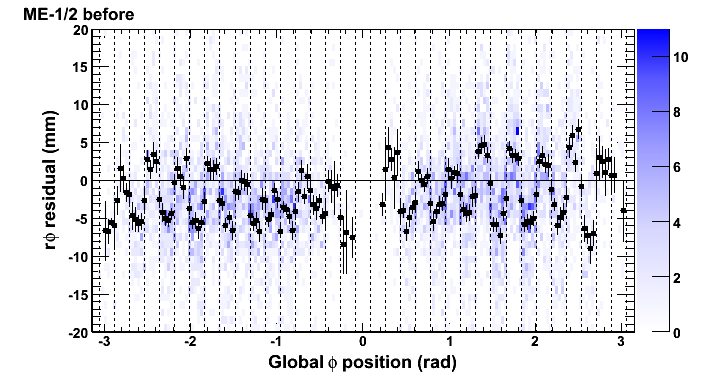
\includegraphics[width=\linewidth]{wasitthepropagator_before.png}

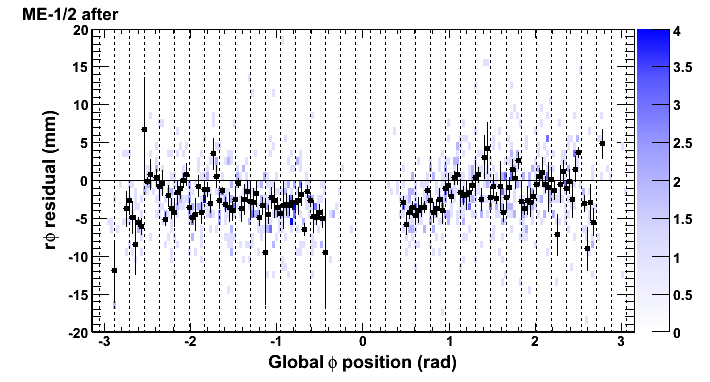
\includegraphics[width=\linewidth]{wasitthepropagator_after.png}
\column{0.35\linewidth}
\begin{itemize}
\item Non-physical alternation of residuals from one chamber to the next stood in the way of alignment

\item $p_T > 40$~GeV cut $\to$ $p_T > 100$~GeV suppresses the effect

\item Not observed in RecHits (overlaps)

\item Unclear what the effect is (not $\vec{B}(\vec{x})$)

\item But it is now possible to perform alignment
\end{itemize}
\end{columns}
\end{frame}

\begin{frame}
\frametitle{CRAFT-2009 alignment}
\begin{itemize}\setlength{\itemsep}{0.3 cm}
\item Two-step procedure:
\begin{enumerate}
\item $Z$ and local $\phi_x$ from link and endcap hardware alignment
\item global $X$, $Y$, $\phi_Z$ of rings from tracks (combined into fits vs.~$\phi$)
\end{enumerate}

\item Tracks are very sensitive to (2) and 2009 data is sufficiently uniform in $\phi$ for robust alignment

\item Not enough tracks to individually align chambers
\begin{itemize}
\item tested machinery and it works, but so few chambers can be aligned that it doesn't make much difference
\end{itemize}

\item Status:
\begin{itemize}
\item SQLite from (1) should be delivered today, tested signs ($\pm$)
\item also waiting for tracker alignment update to start (2)
\end{itemize}

\item Preliminary results follow (16 pages), final results will be similar
\end{itemize}
\end{frame}

\begin{frame}
\frametitle{Ring fits: ME$-$4/1}
\vfill
\begin{columns}
\column{0.7\linewidth}
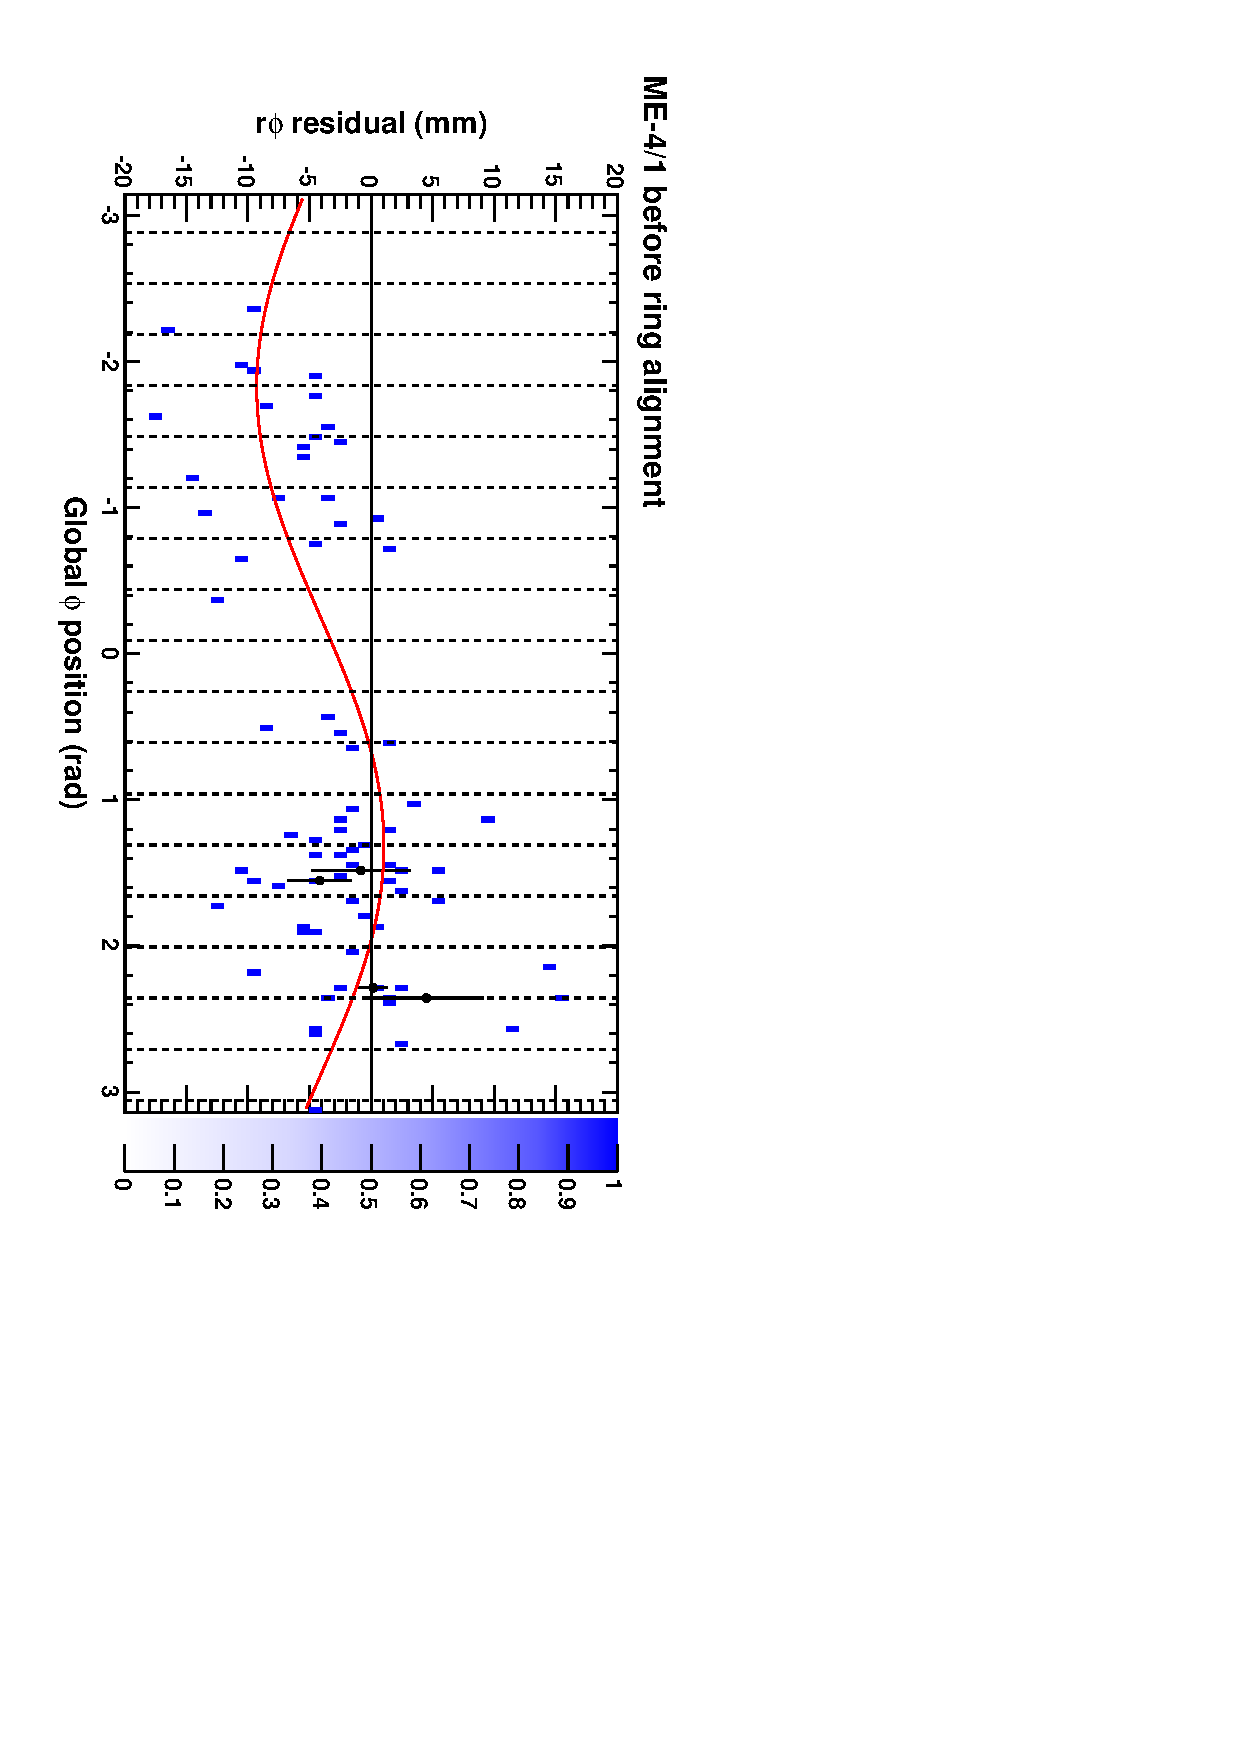
\includegraphics[height=\linewidth, angle=90]{ringfits_before/mem41.pdf}

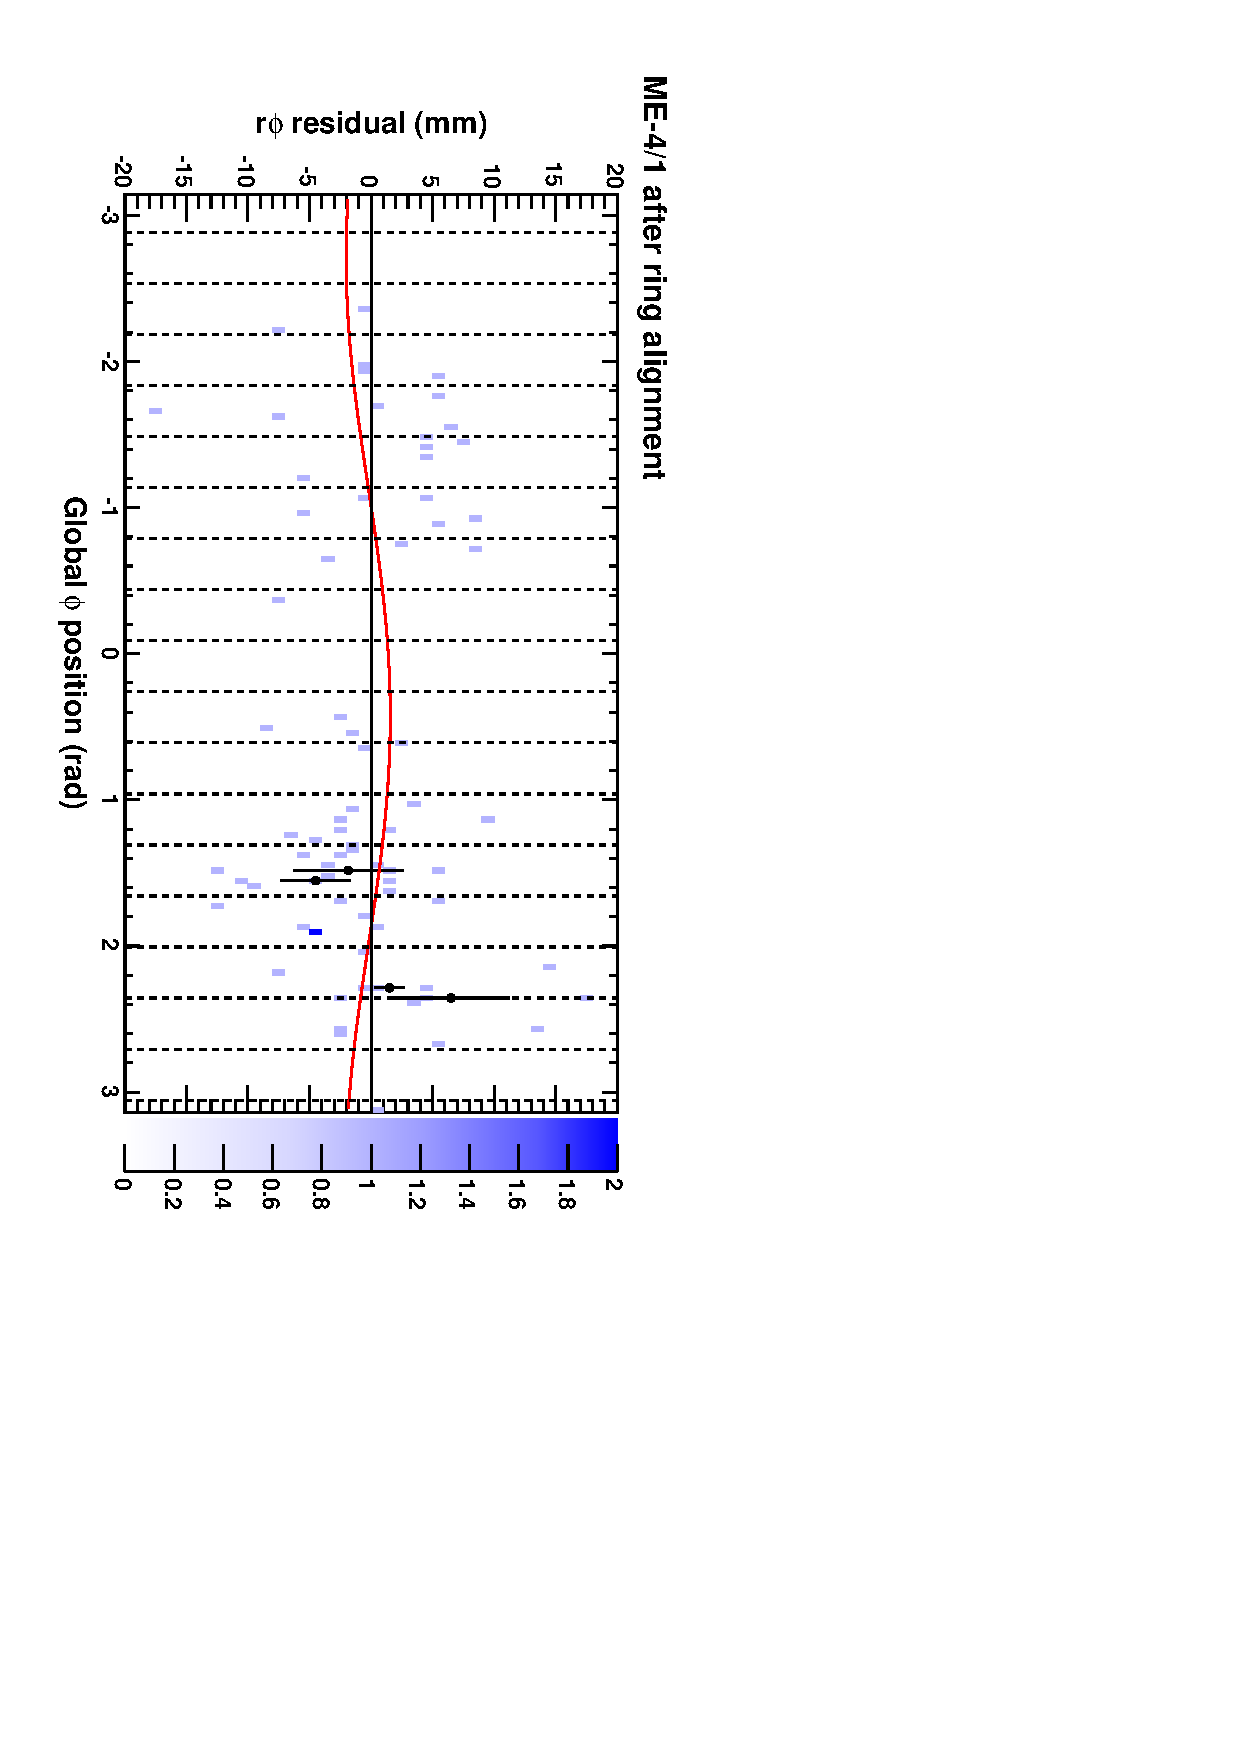
\includegraphics[height=\linewidth, angle=90]{ringfits_after/mem41.pdf}
\column{0.3\linewidth}
\begin{itemize}
\item Unbiased residuals from tracker tracks
\item Color scale is 2-D plot
\item Black points are a profile (averages in vertical bins)
\item Red line is fit to 2-D data
\item sine $\sim$ $X$ \\
cosine $\sim$ $Y$ \\
constant $\sim$ $\phi_Z$
\end{itemize}
\end{columns}
\end{frame}

\begin{frame}
\frametitle{Ring fits: ME$-$3/2}
\vfill
\begin{columns}
\column{0.7\linewidth}
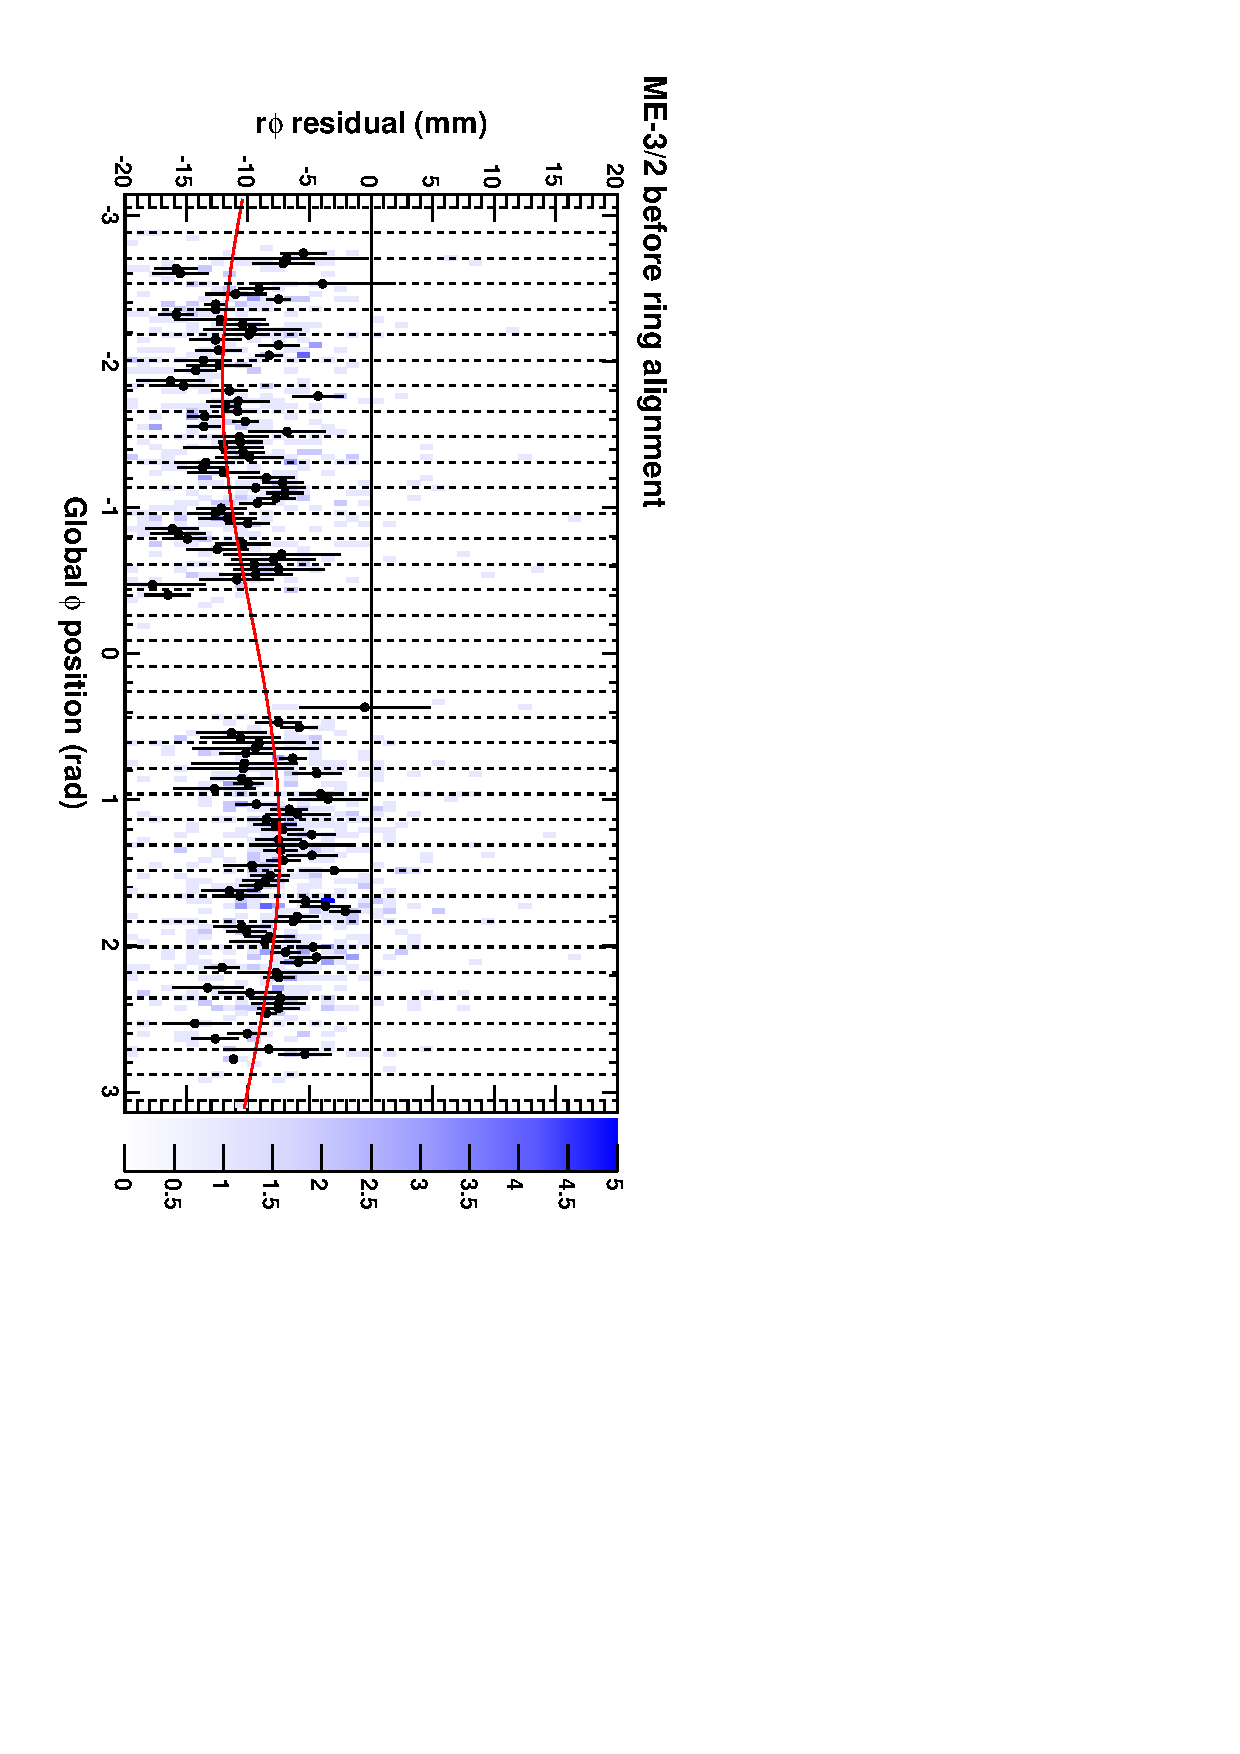
\includegraphics[height=\linewidth, angle=90]{ringfits_before/mem32.pdf}

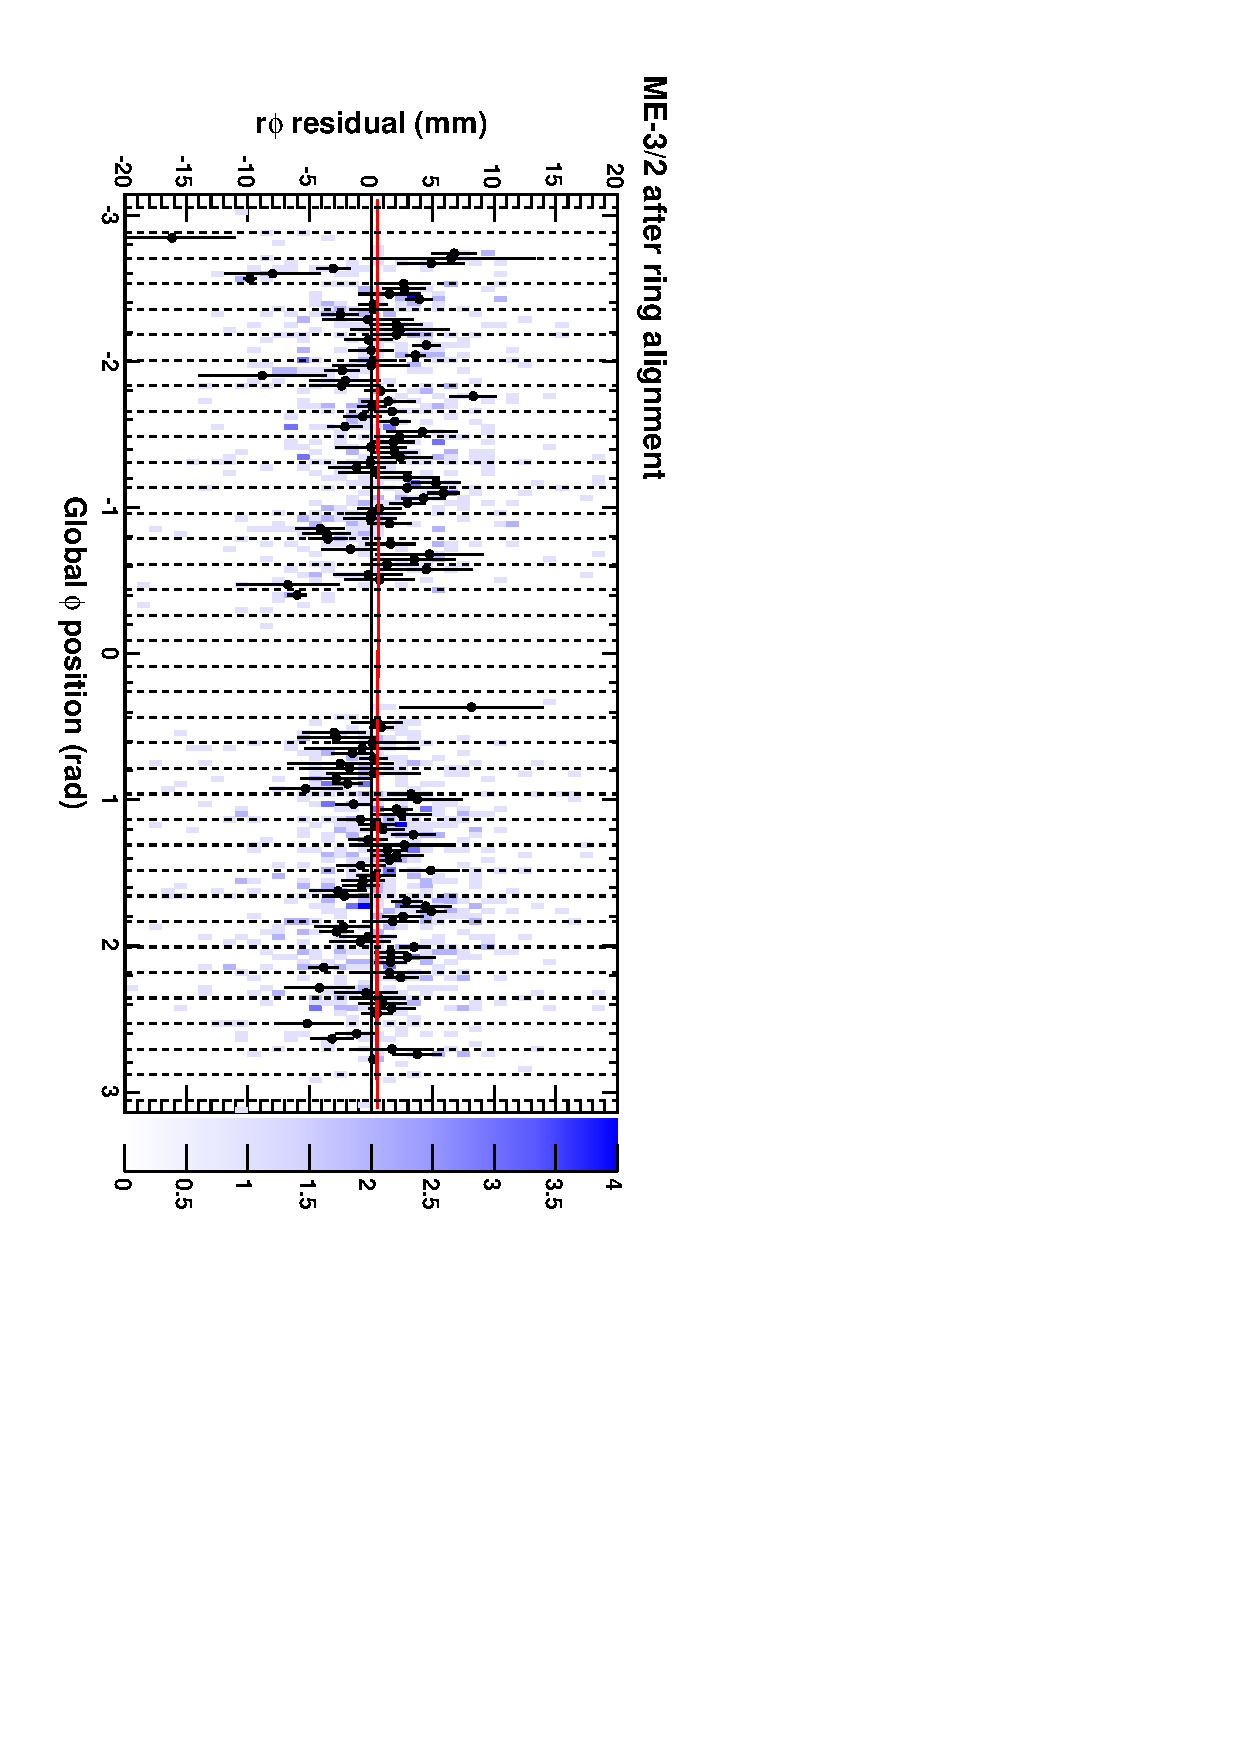
\includegraphics[height=\linewidth, angle=90]{ringfits_after/mem32.pdf}
\column{0.3\linewidth}
\begin{itemize}
\item Unbiased residuals from tracker tracks
\item Color scale is 2-D plot
\item Black points are a profile (averages in vertical bins)
\item Red line is fit to 2-D data
\item sine $\sim$ $X$ \\
cosine $\sim$ $Y$ \\
constant $\sim$ $\phi_Z$
\end{itemize}
\end{columns}
\end{frame}

\begin{frame}
\frametitle{Ring fits: ME$-$3/1}
\vfill
\begin{columns}
\column{0.7\linewidth}
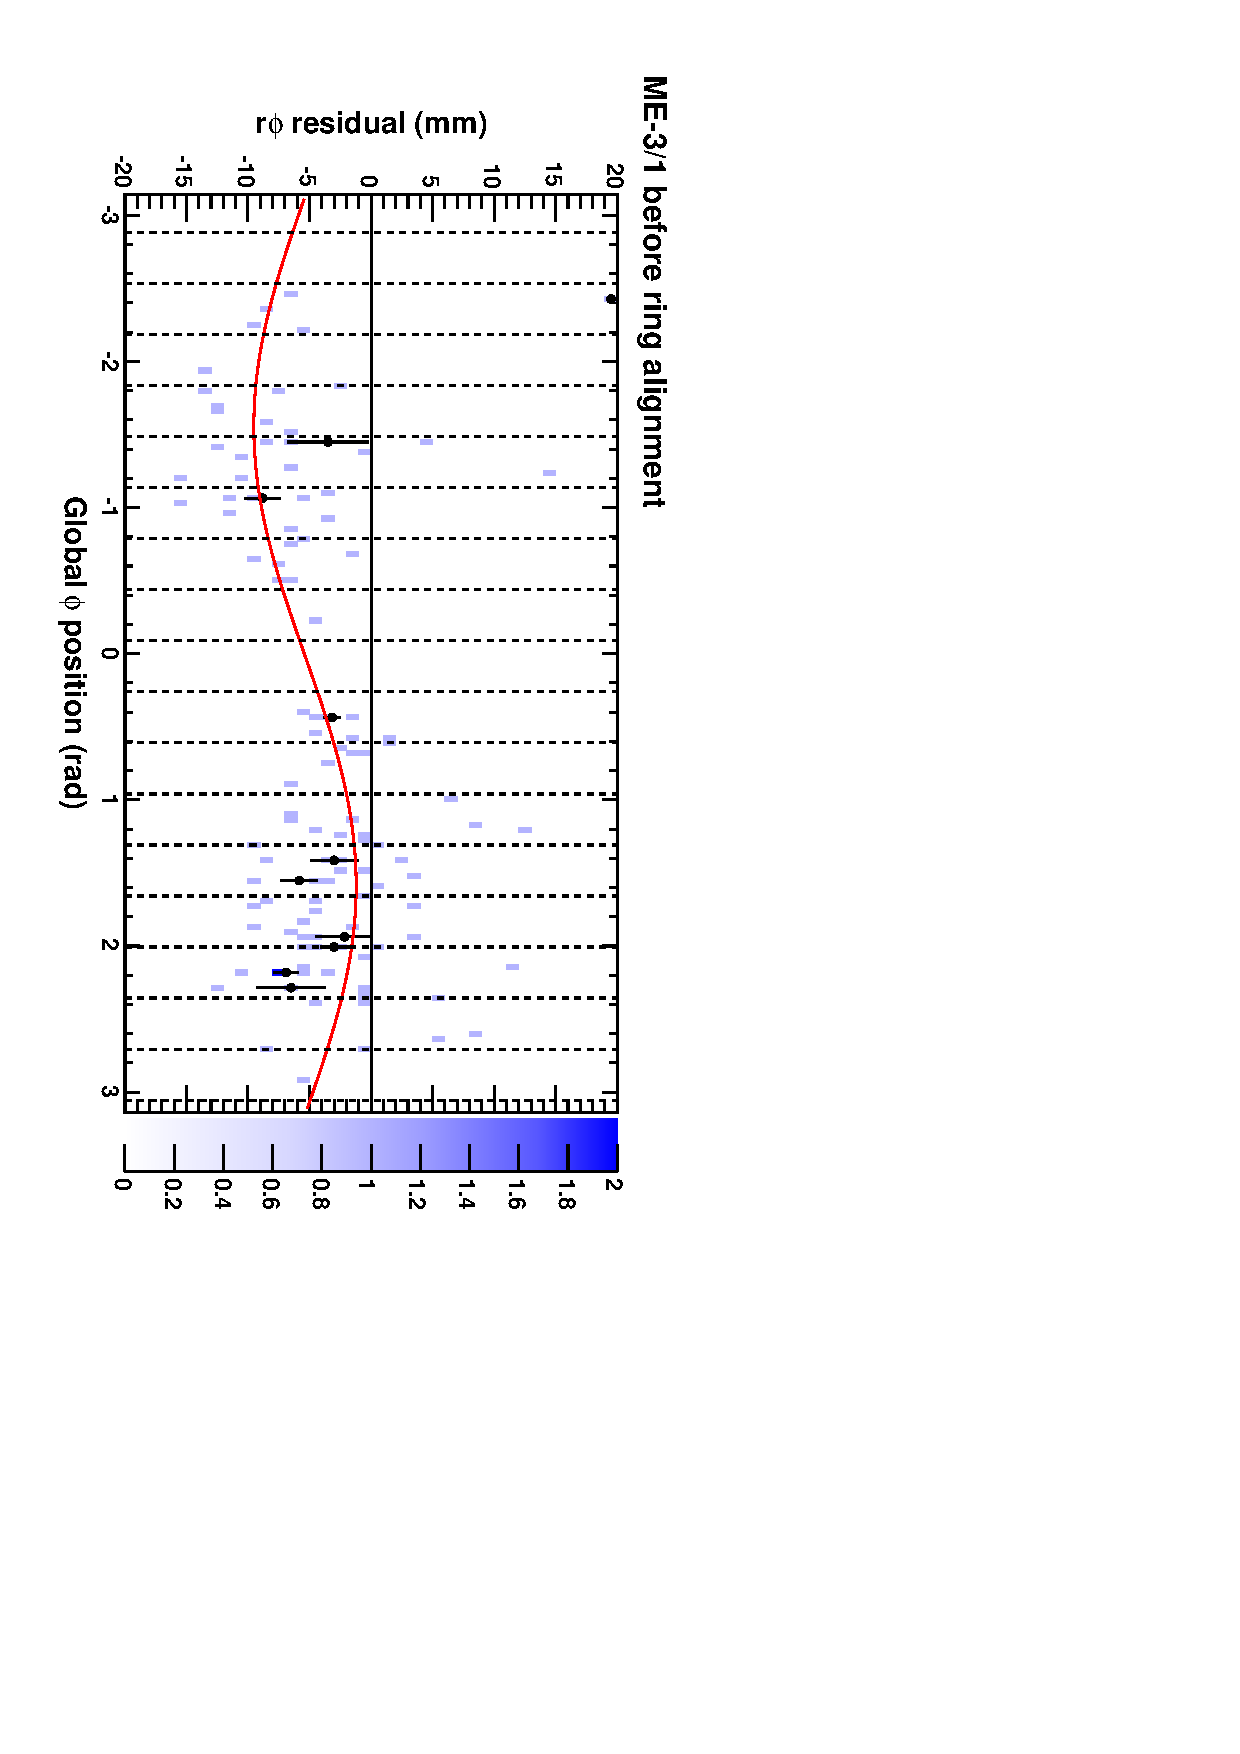
\includegraphics[height=\linewidth, angle=90]{ringfits_before/mem31.pdf}

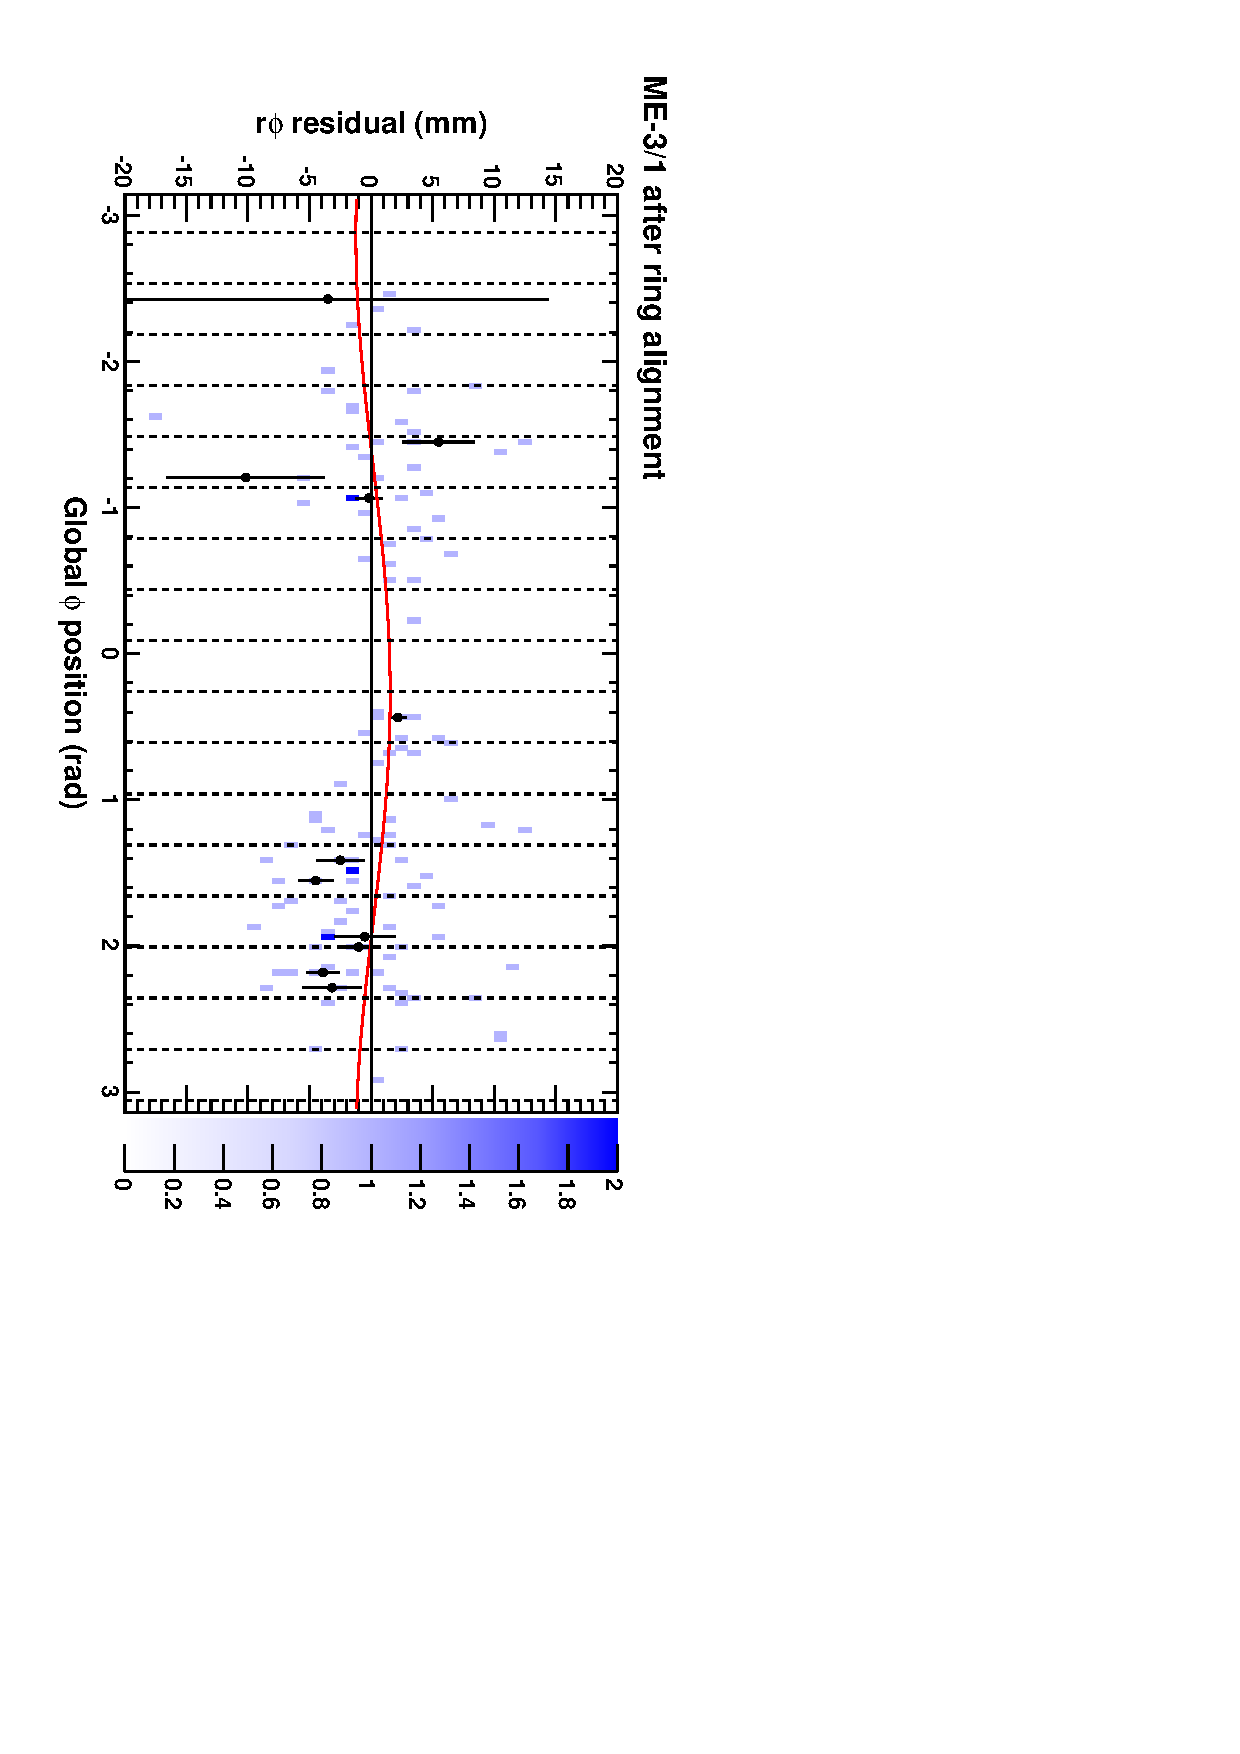
\includegraphics[height=\linewidth, angle=90]{ringfits_after/mem31.pdf}
\column{0.3\linewidth}
\begin{itemize}
\item Unbiased residuals from tracker tracks
\item Color scale is 2-D plot
\item Black points are a profile (averages in vertical bins)
\item Red line is fit to 2-D data
\item sine $\sim$ $X$ \\
cosine $\sim$ $Y$ \\
constant $\sim$ $\phi_Z$
\end{itemize}
\end{columns}
\end{frame}

\begin{frame}
\frametitle{Ring fits: ME$-$2/2}
\vfill
\begin{columns}
\column{0.7\linewidth}
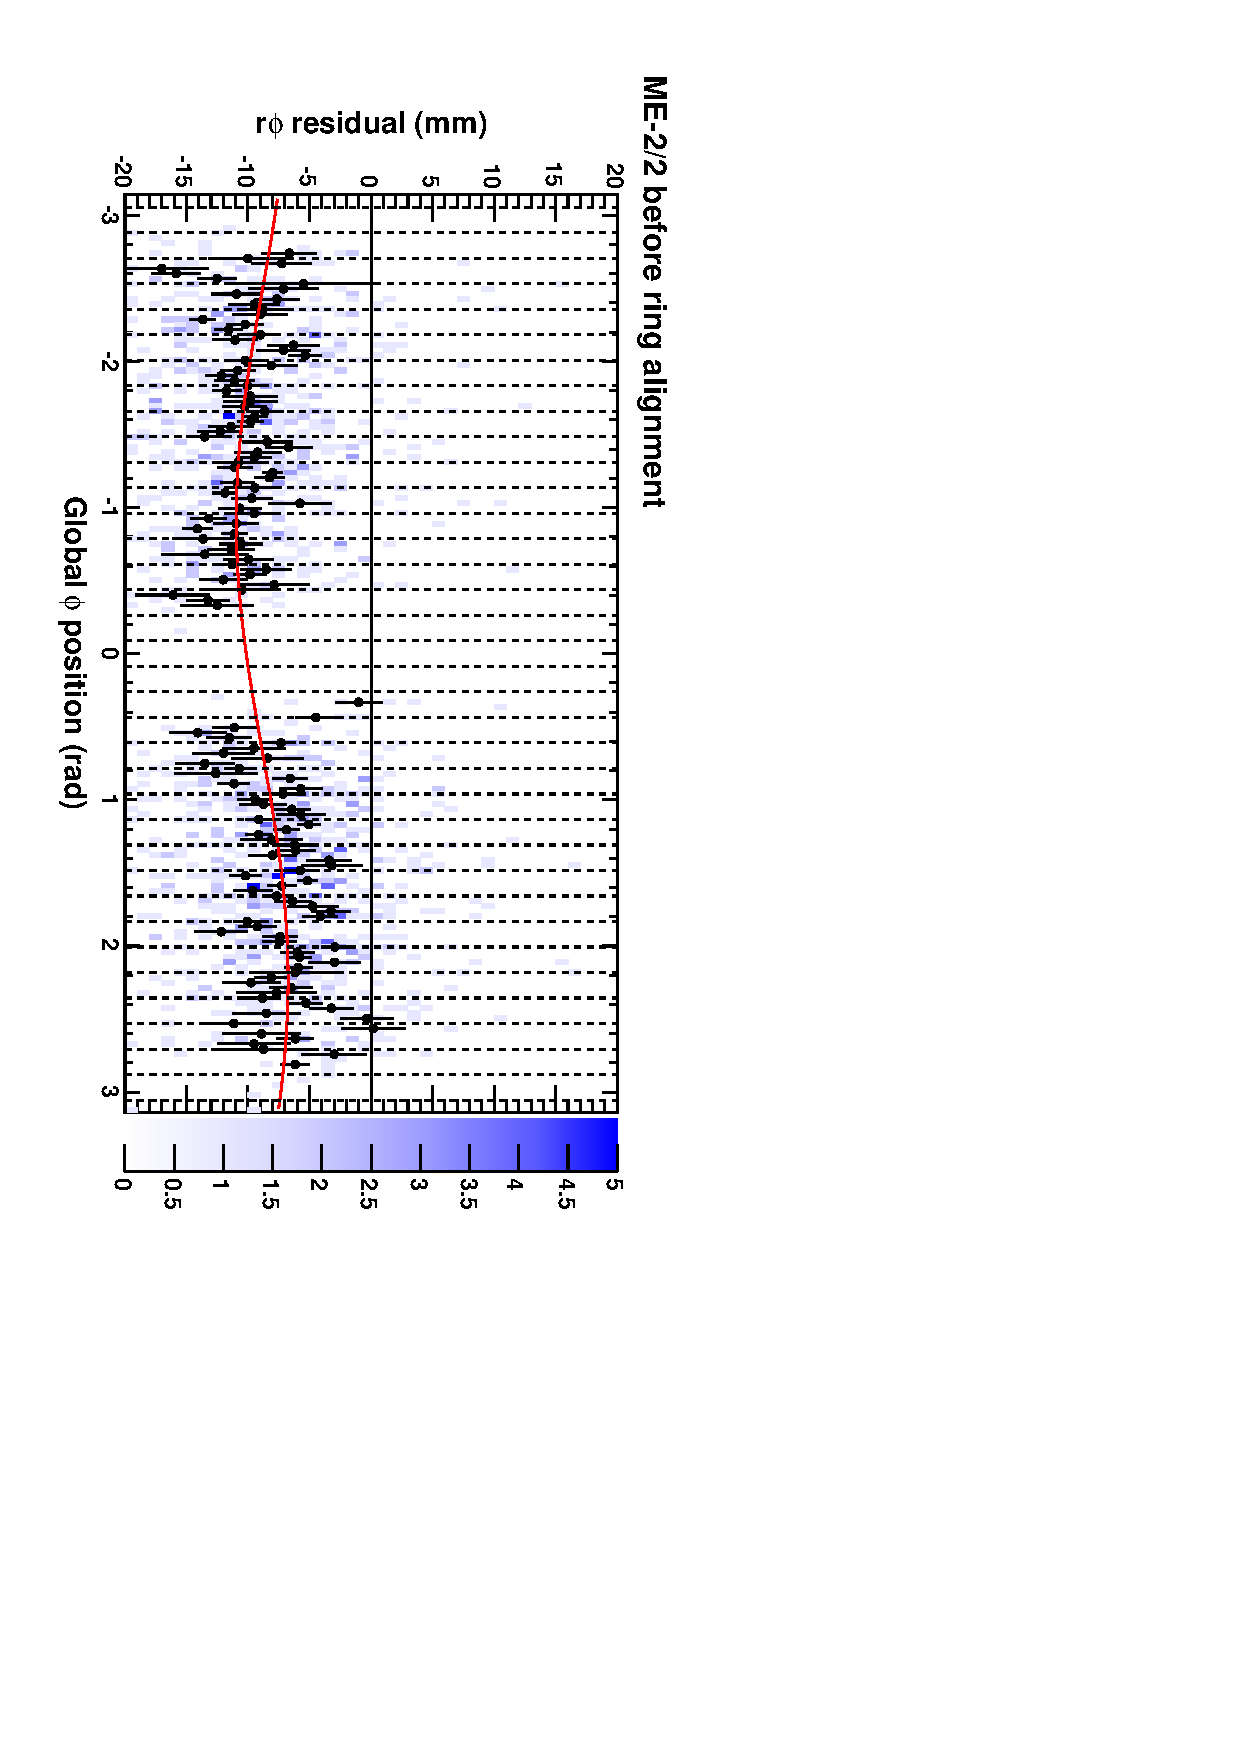
\includegraphics[height=\linewidth, angle=90]{ringfits_before/mem22.pdf}

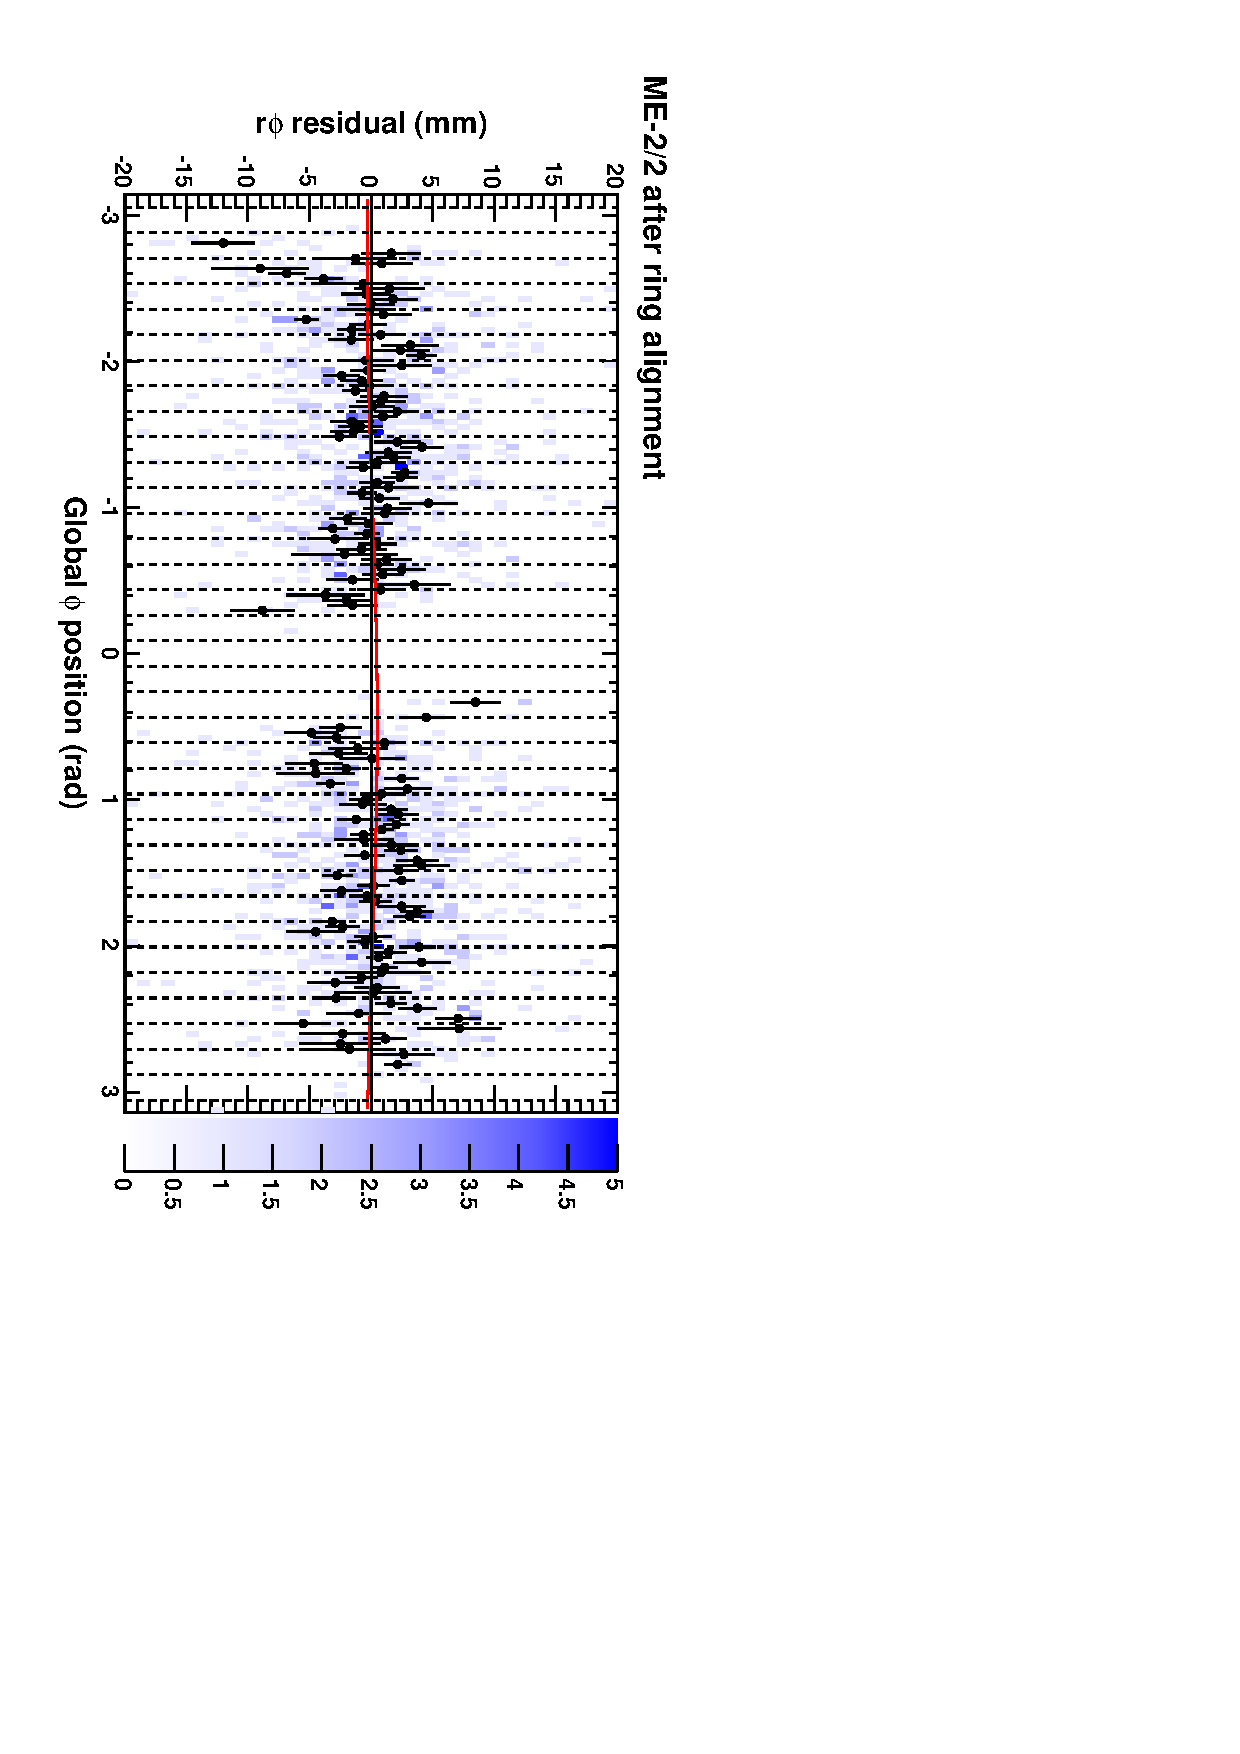
\includegraphics[height=\linewidth, angle=90]{ringfits_after/mem22.pdf}
\column{0.3\linewidth}
\begin{itemize}
\item Unbiased residuals from tracker tracks
\item Color scale is 2-D plot
\item Black points are a profile (averages in vertical bins)
\item Red line is fit to 2-D data
\item sine $\sim$ $X$ \\
cosine $\sim$ $Y$ \\
constant $\sim$ $\phi_Z$
\end{itemize}
\end{columns}
\end{frame}

\begin{frame}
\frametitle{Ring fits: ME$-$2/1}
\vfill
\begin{columns}
\column{0.7\linewidth}
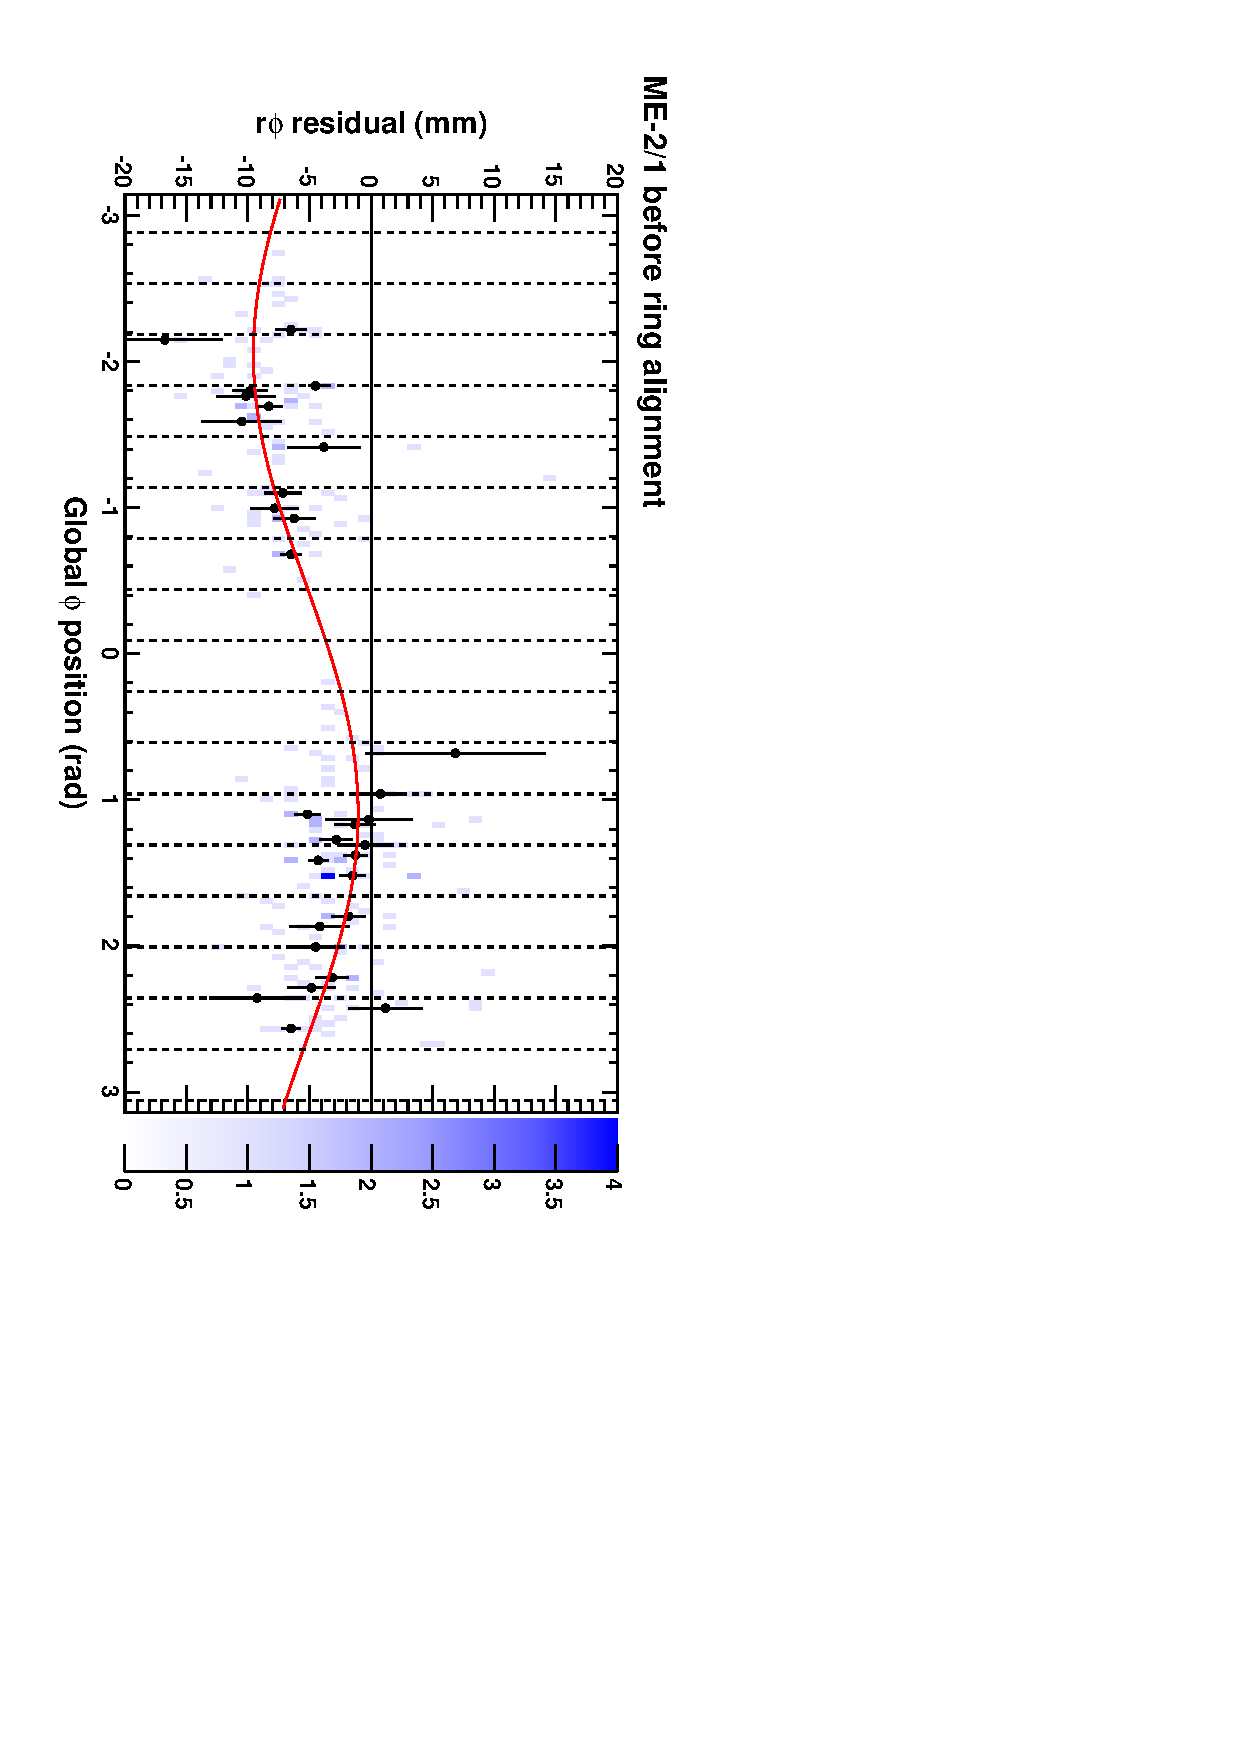
\includegraphics[height=\linewidth, angle=90]{ringfits_before/mem21.pdf}

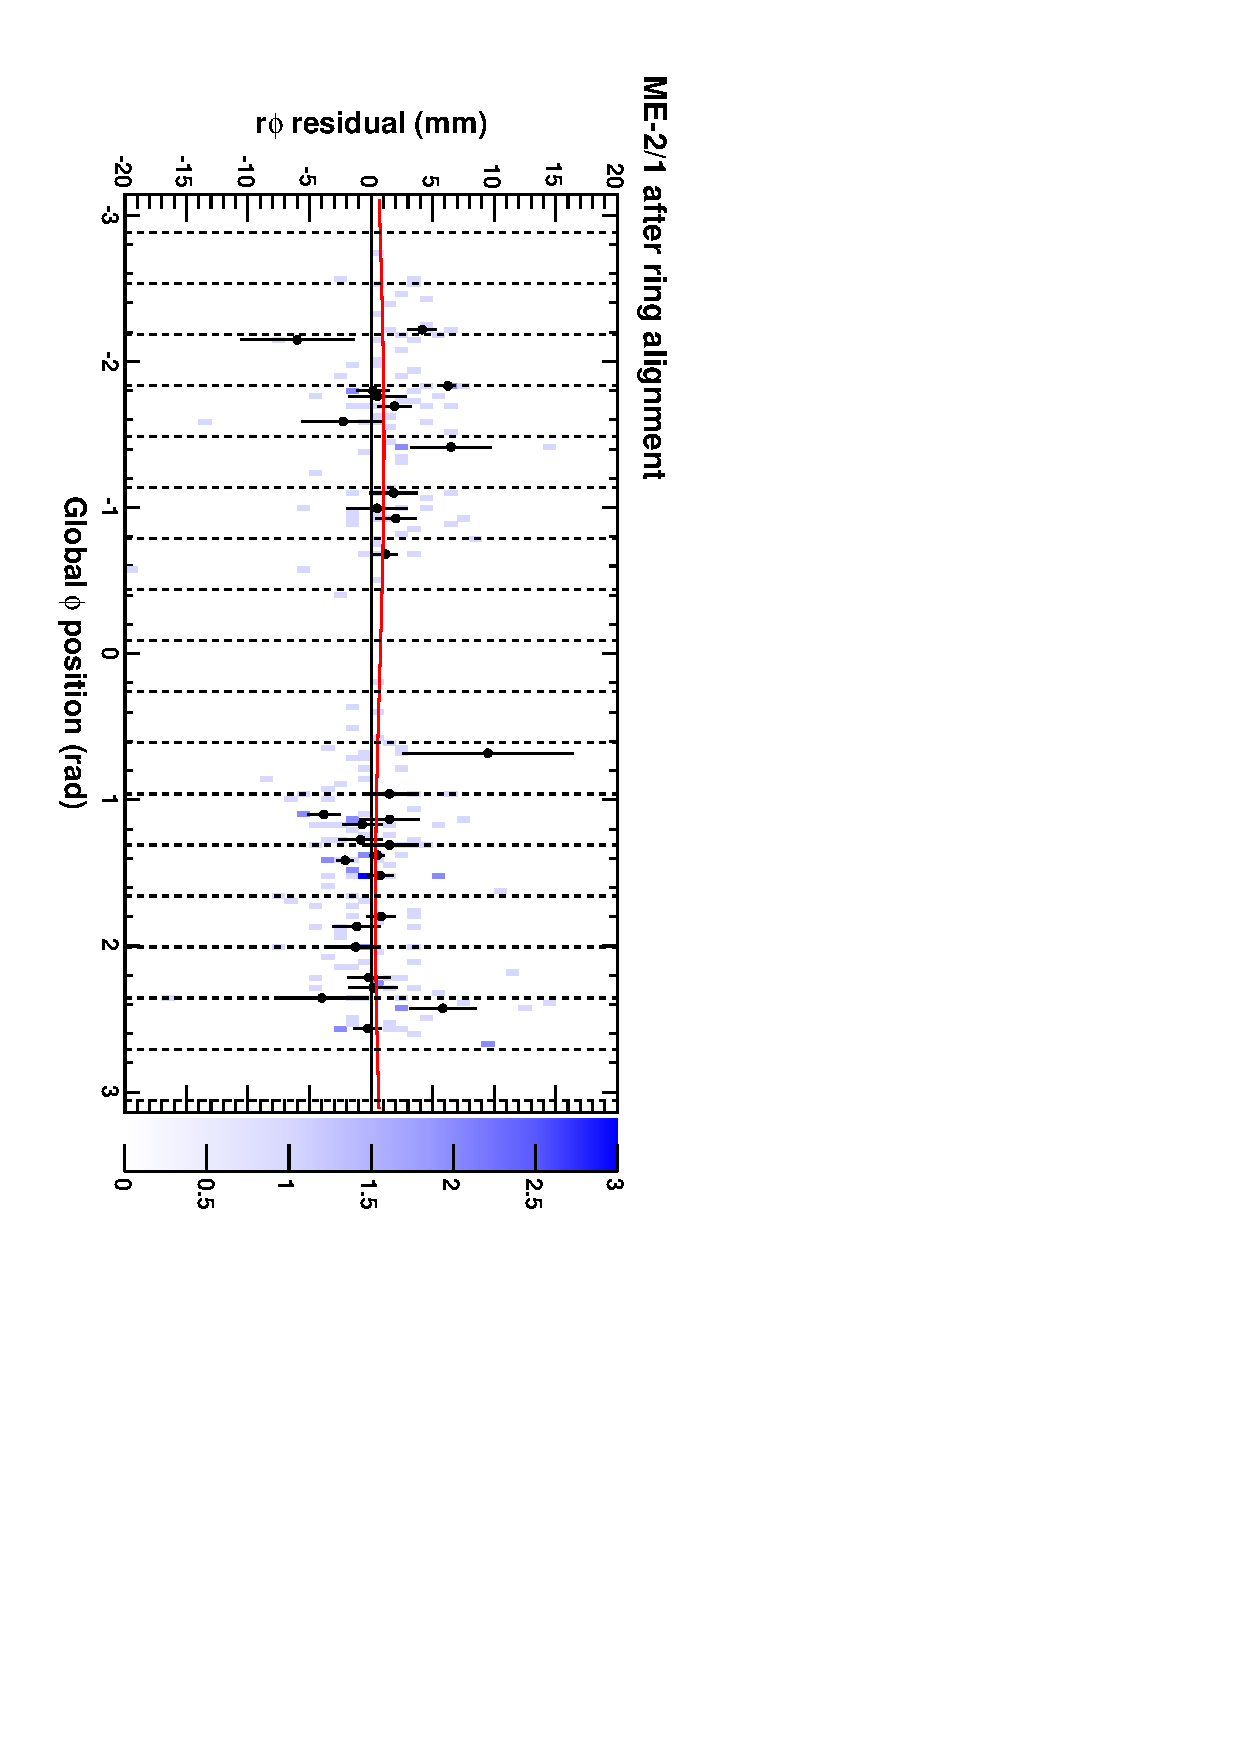
\includegraphics[height=\linewidth, angle=90]{ringfits_after/mem21.pdf}
\column{0.3\linewidth}
\begin{itemize}
\item Unbiased residuals from tracker tracks
\item Color scale is 2-D plot
\item Black points are a profile (averages in vertical bins)
\item Red line is fit to 2-D data
\item sine $\sim$ $X$ \\
cosine $\sim$ $Y$ \\
constant $\sim$ $\phi_Z$
\end{itemize}
\end{columns}
\end{frame}

\begin{frame}
\frametitle{Ring fits: ME$-$1/3}
\vfill
\begin{columns}
\column{0.7\linewidth}
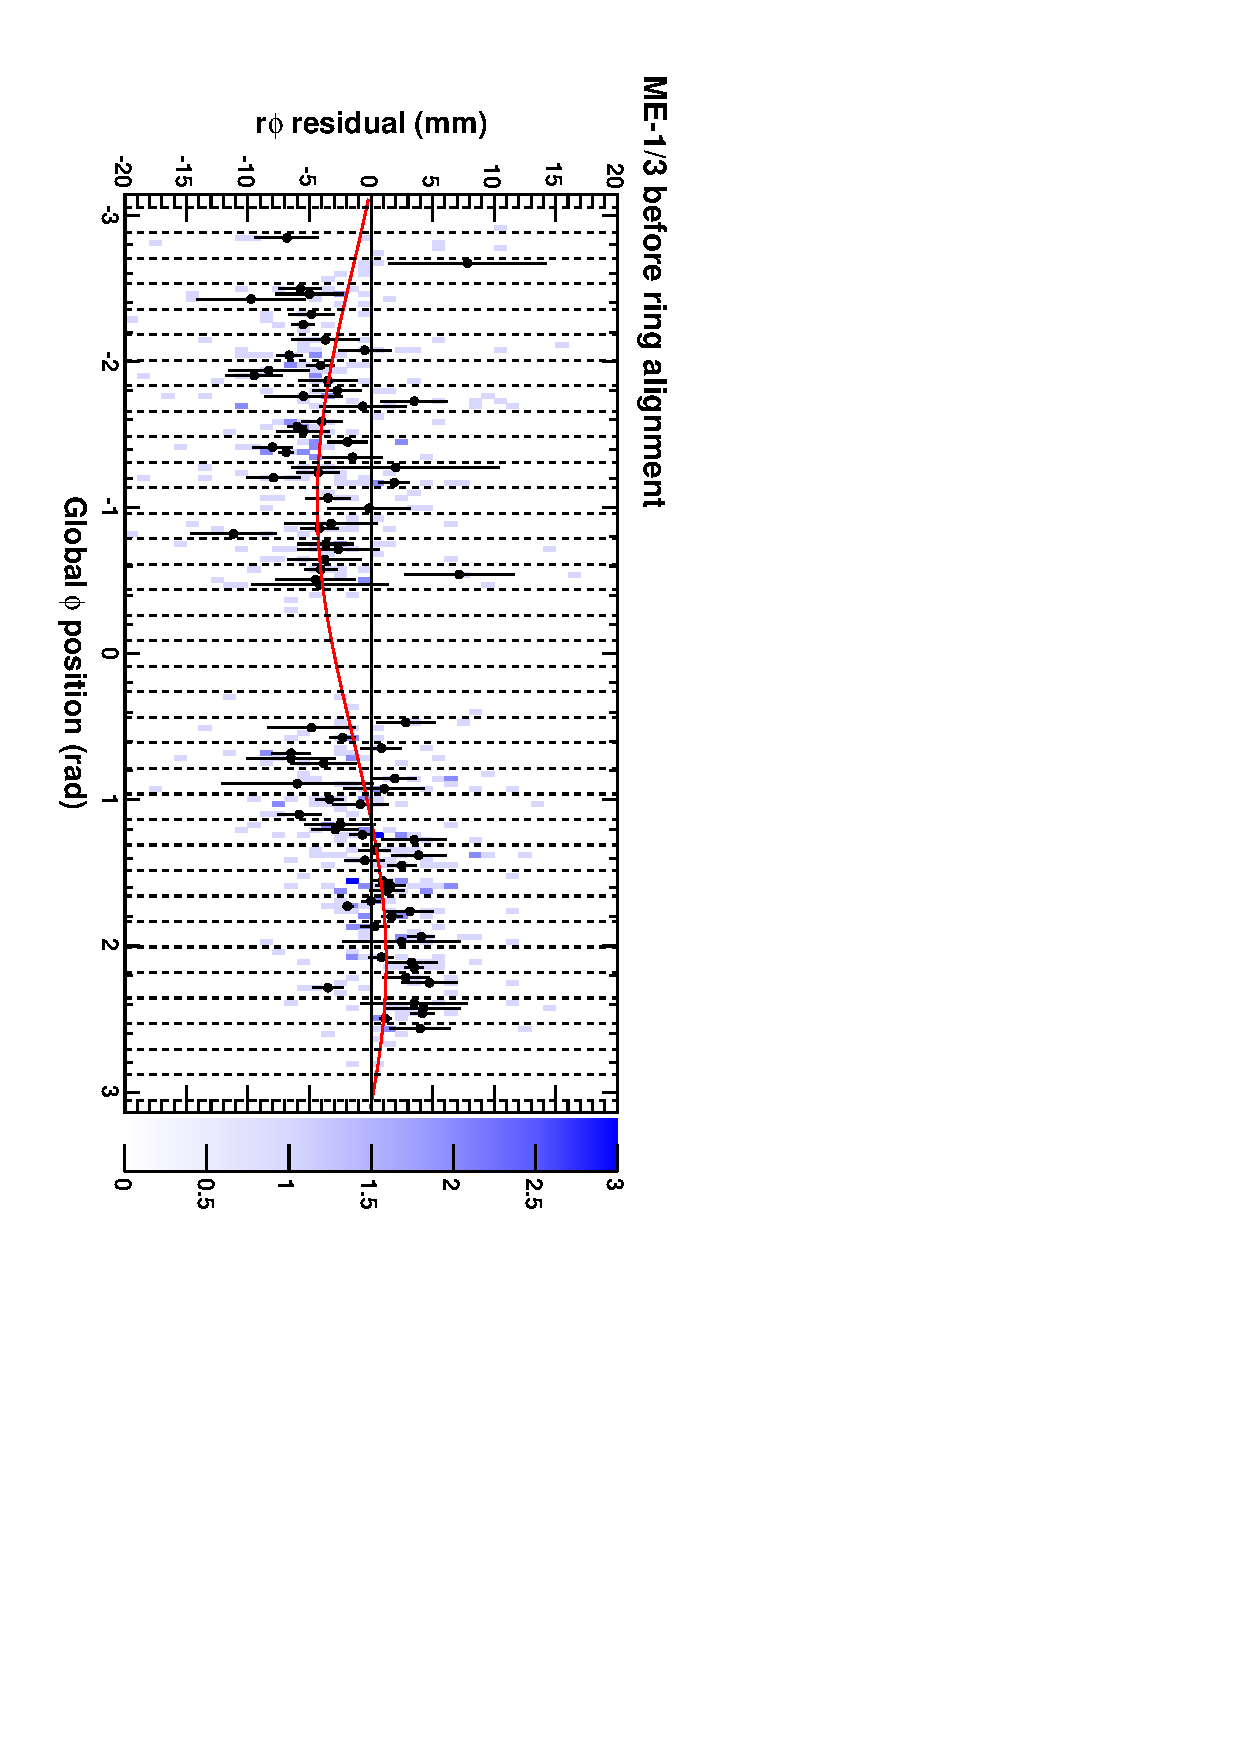
\includegraphics[height=\linewidth, angle=90]{ringfits_before/mem13.pdf}

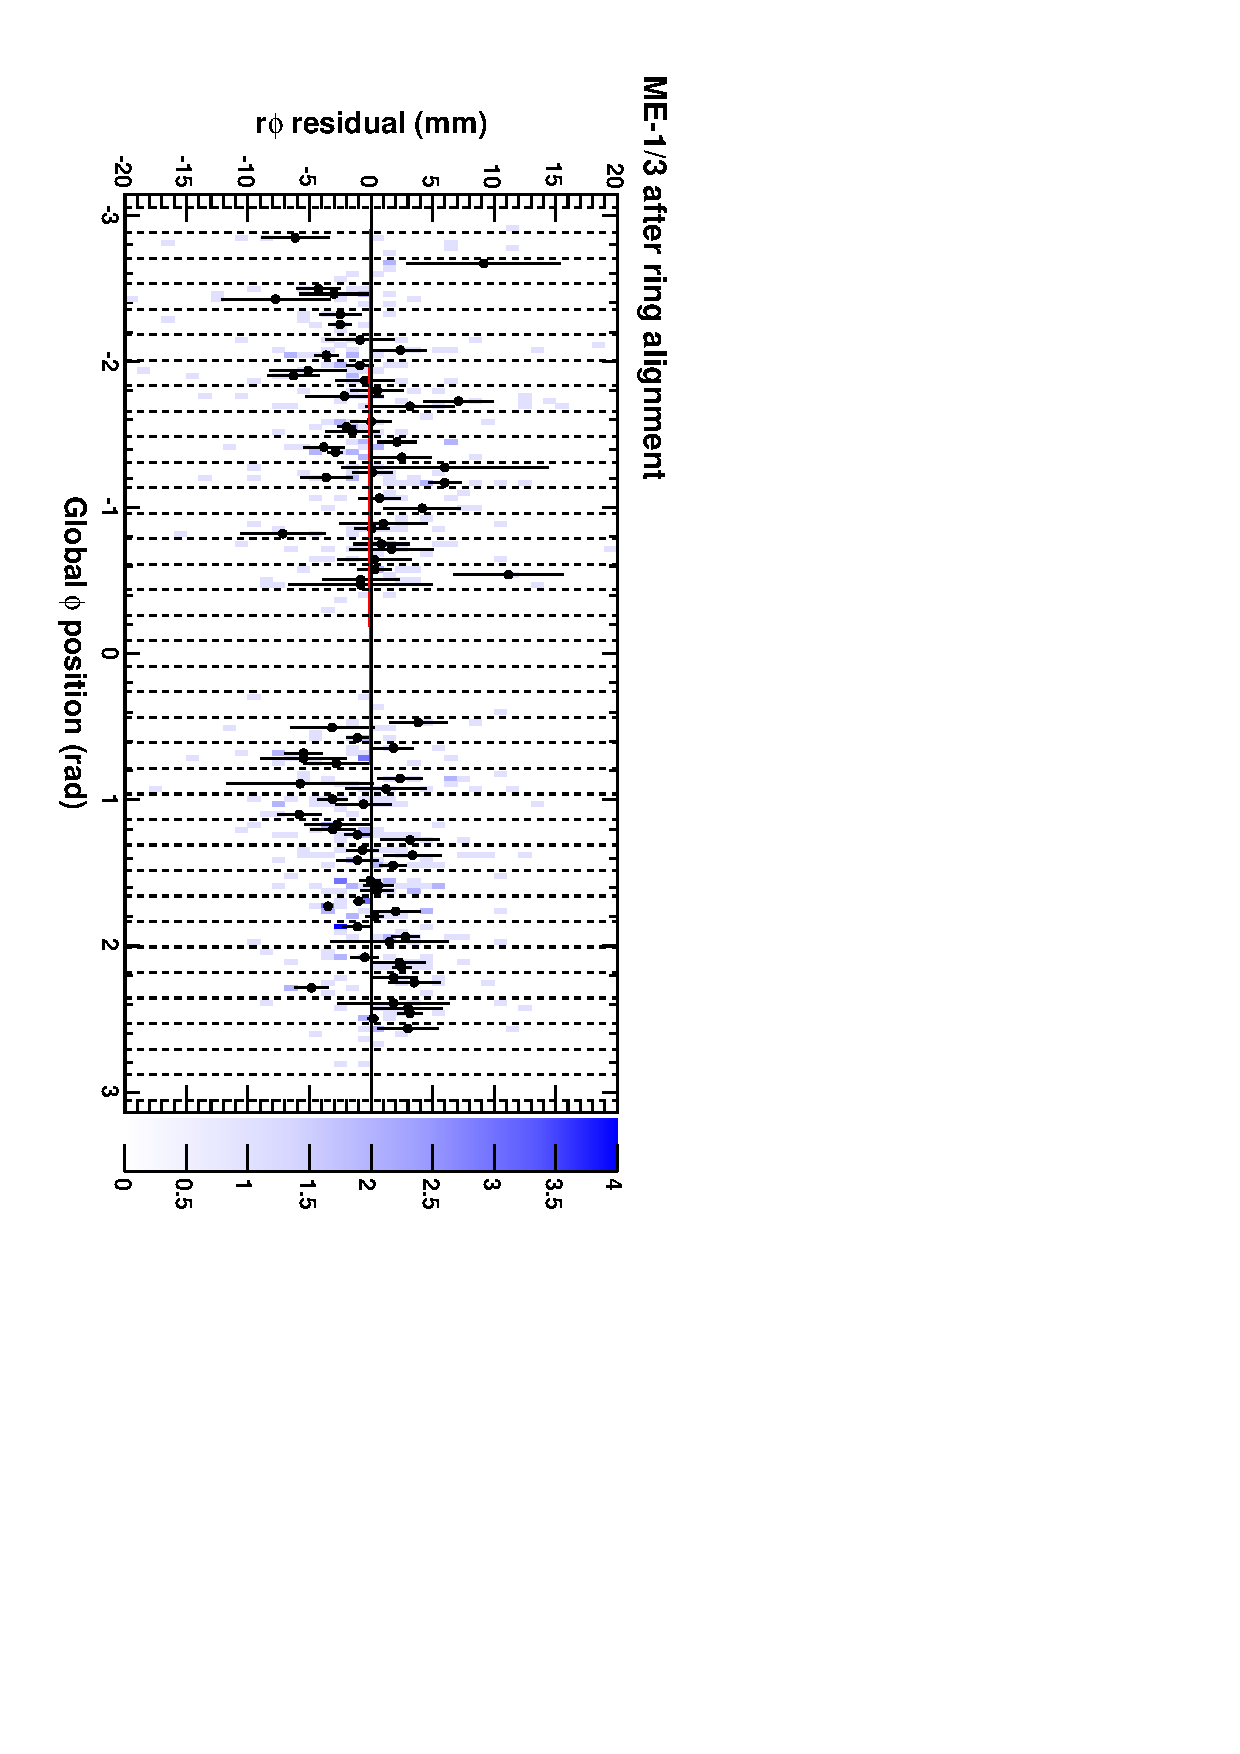
\includegraphics[height=\linewidth, angle=90]{ringfits_after/mem13.pdf}
\column{0.3\linewidth}
\begin{itemize}
\item Unbiased residuals from tracker tracks
\item Color scale is 2-D plot
\item Black points are a profile (averages in vertical bins)
\item Red line is fit to 2-D data
\item sine $\sim$ $X$ \\
cosine $\sim$ $Y$ \\
constant $\sim$ $\phi_Z$
\end{itemize}
\end{columns}
\end{frame}

\begin{frame}
\frametitle{Ring fits: ME$-$1/2}
\vfill
\begin{columns}
\column{0.7\linewidth}
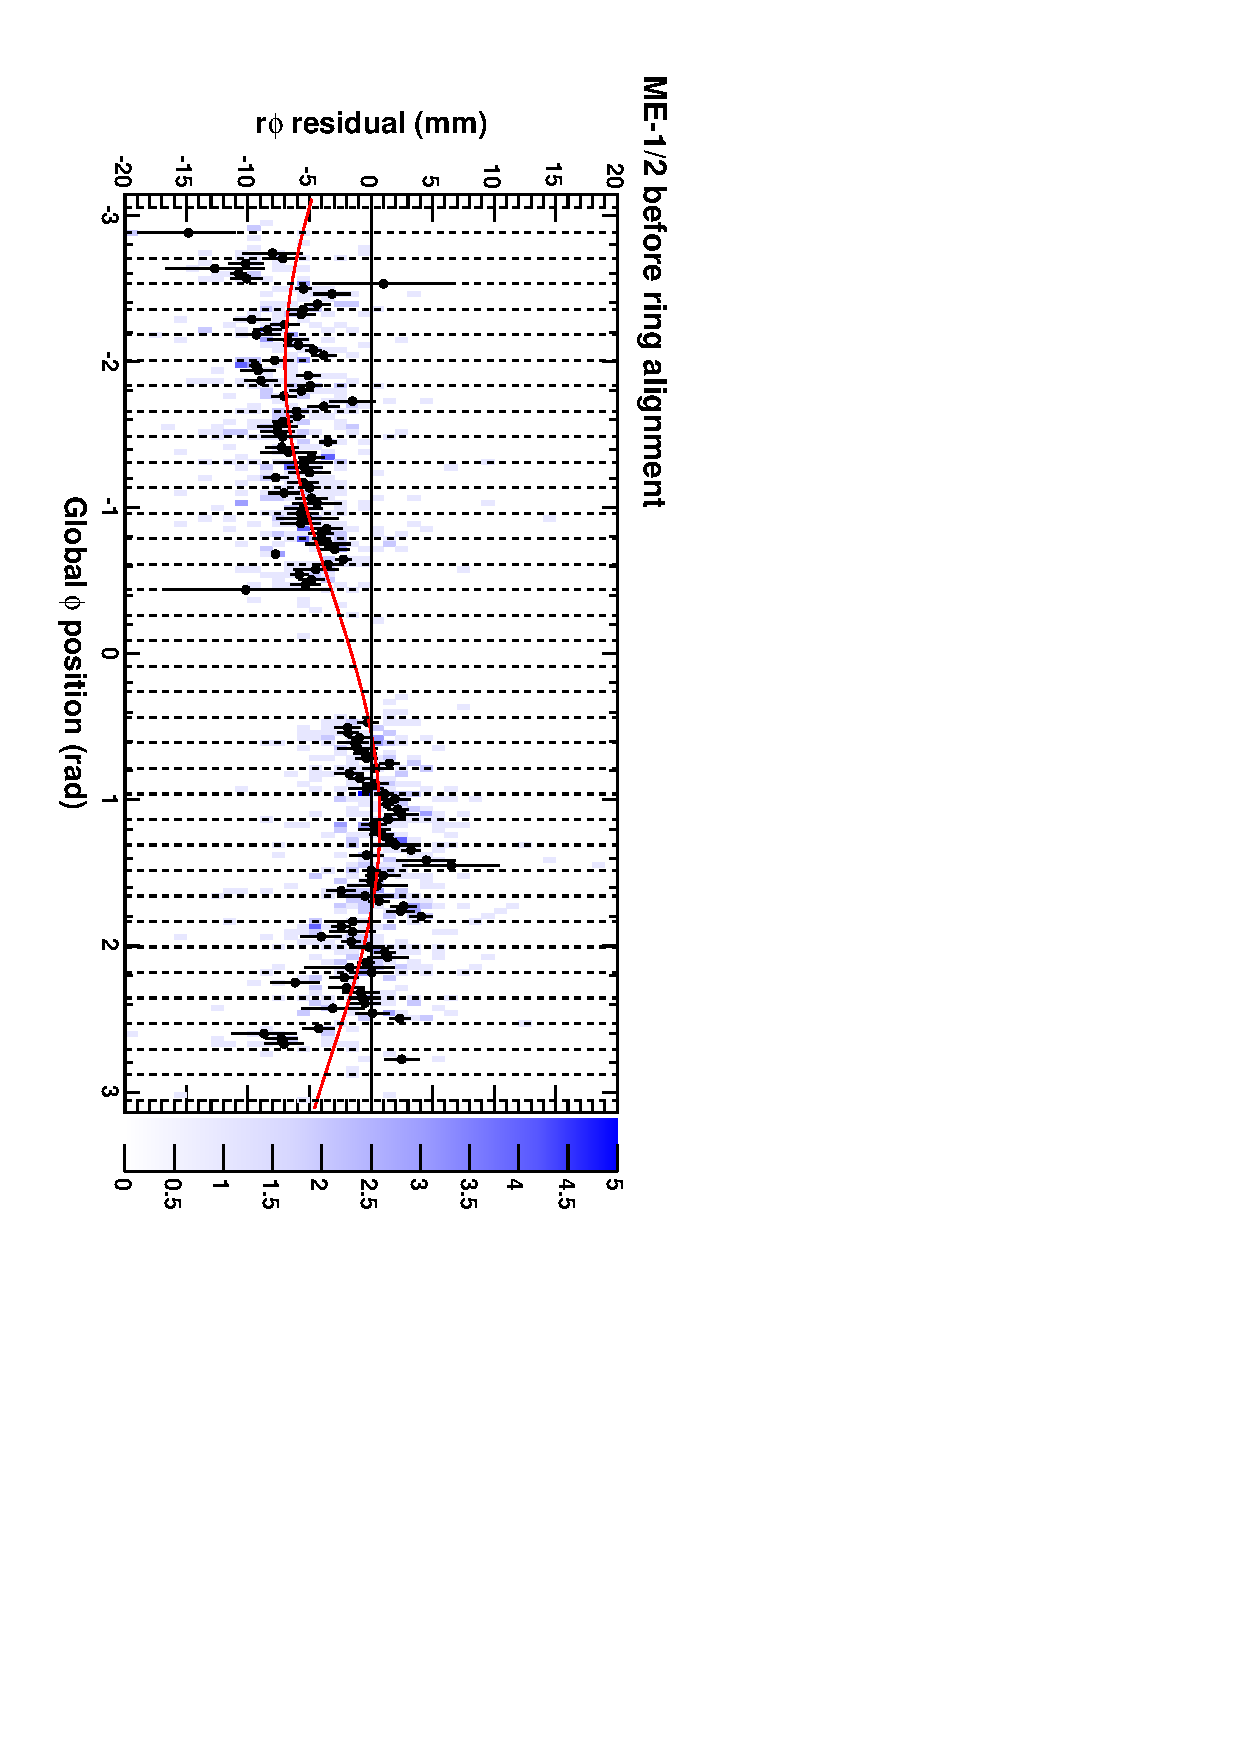
\includegraphics[height=\linewidth, angle=90]{ringfits_before/mem12.pdf}

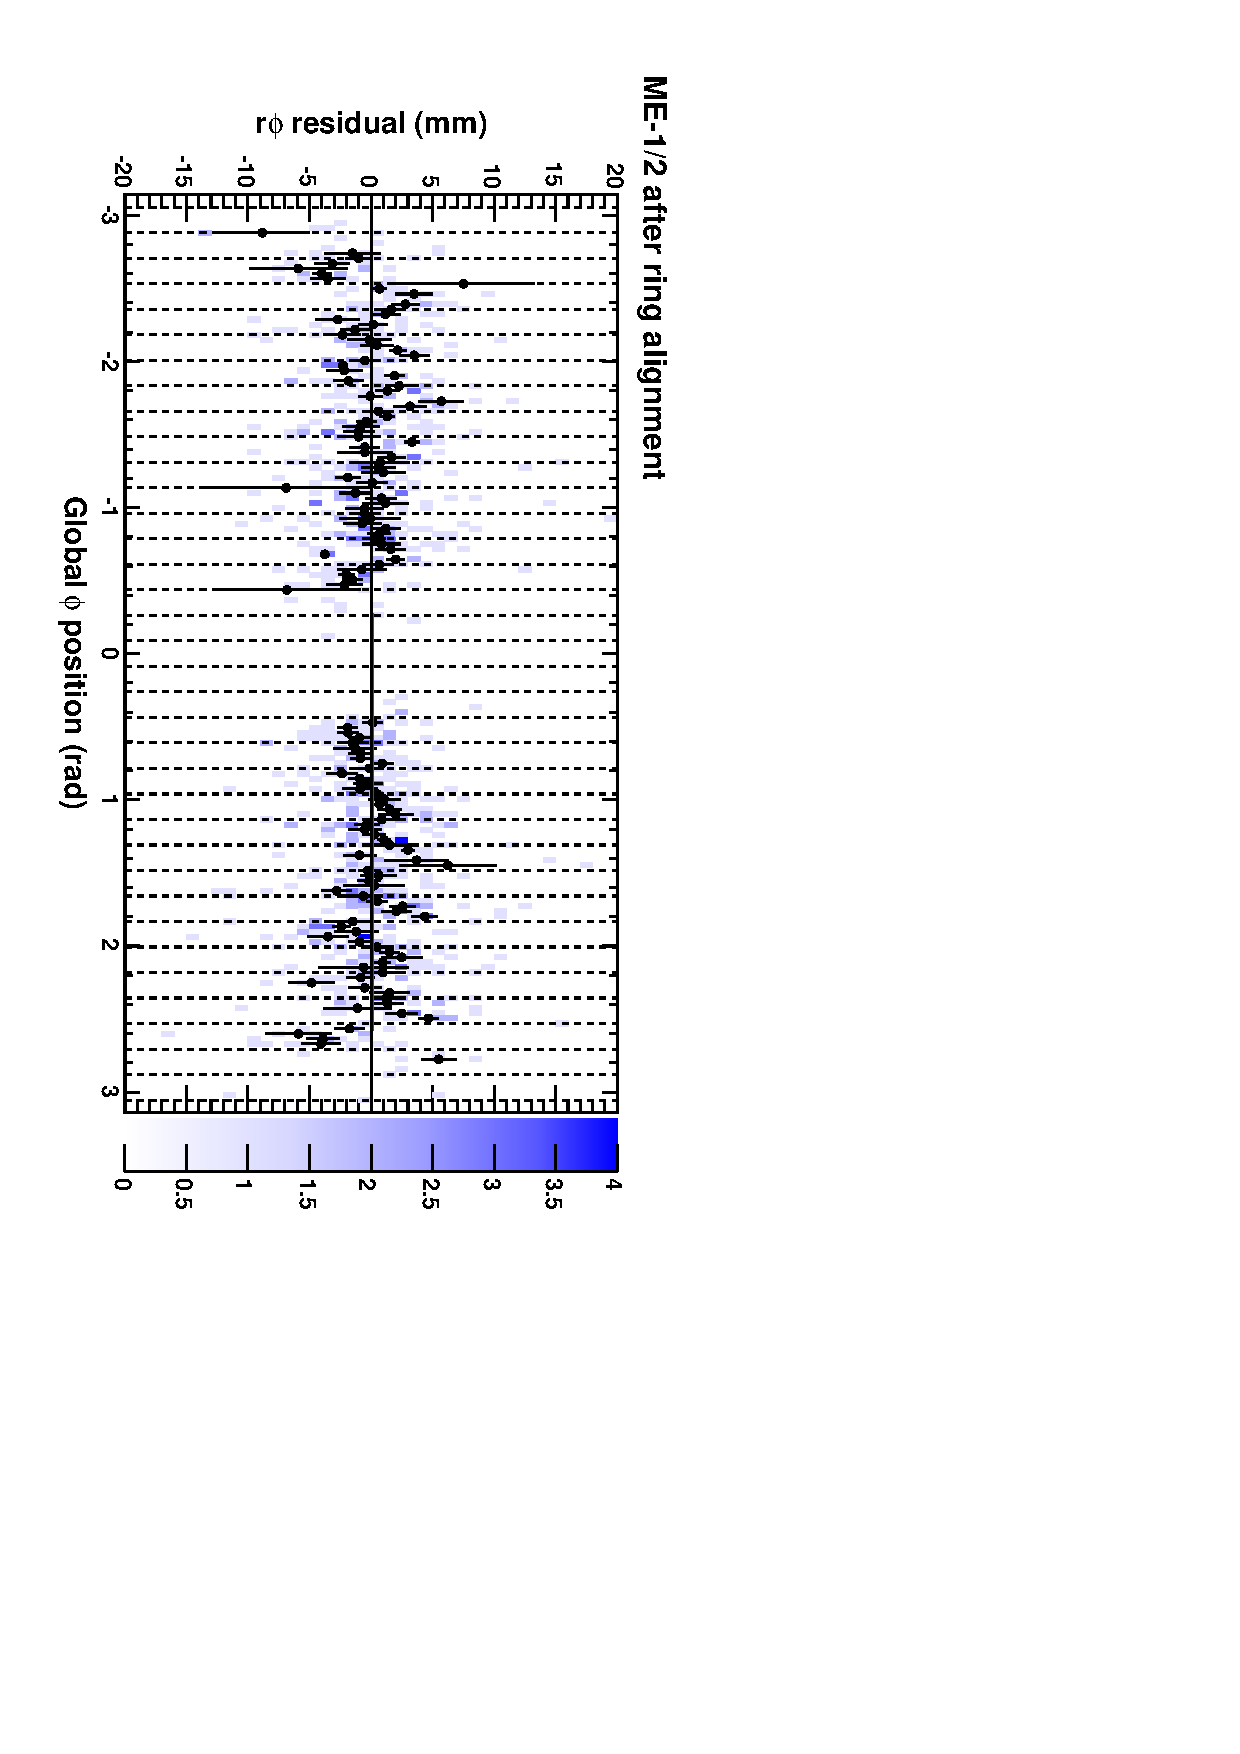
\includegraphics[height=\linewidth, angle=90]{ringfits_after/mem12.pdf}
\column{0.3\linewidth}
\begin{itemize}
\item Unbiased residuals from tracker tracks
\item Color scale is 2-D plot
\item Black points are a profile (averages in vertical bins)
\item Red line is fit to 2-D data
\item sine $\sim$ $X$ \\
cosine $\sim$ $Y$ \\
constant $\sim$ $\phi_Z$
\end{itemize}
\end{columns}
\end{frame}

\begin{frame}
\frametitle{Ring fits: ME$-$1/1}
\vfill
\begin{columns}
\column{0.7\linewidth}
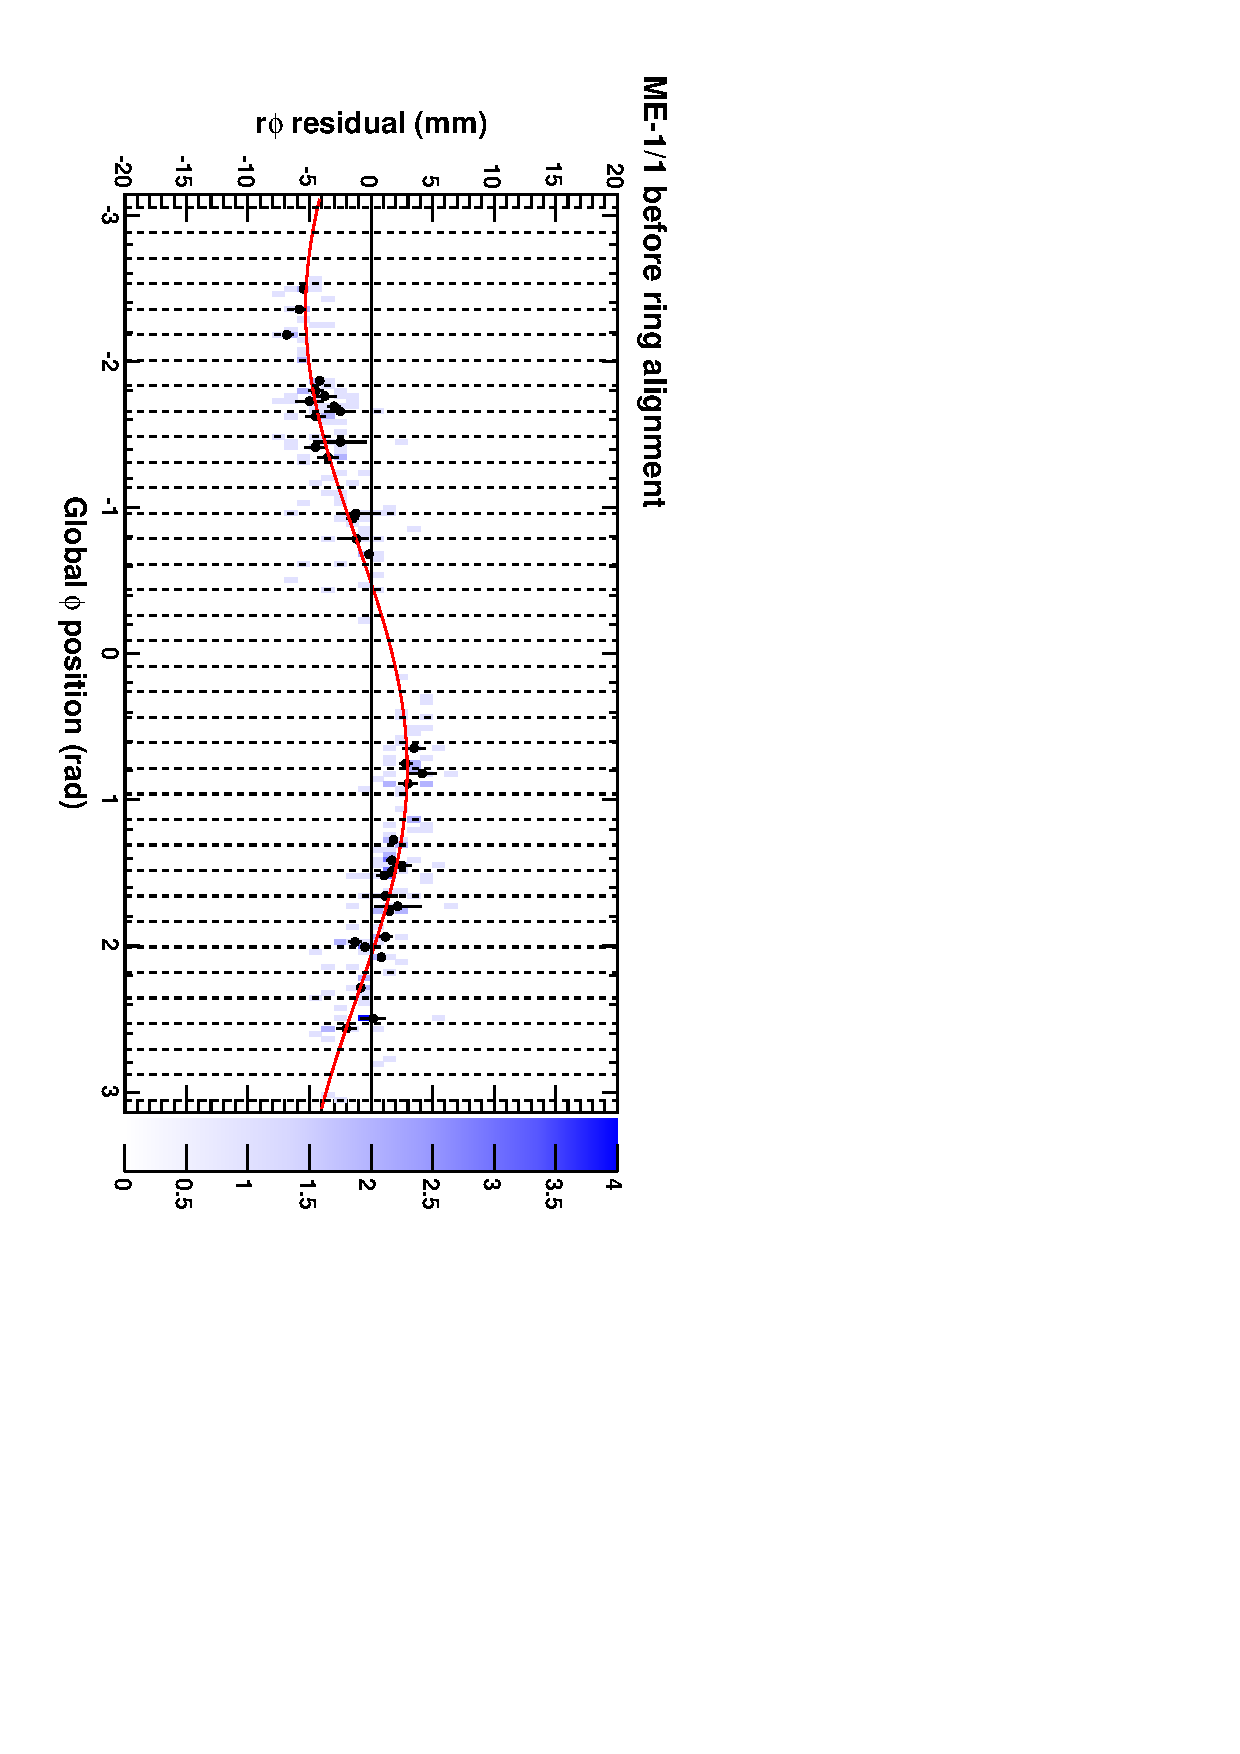
\includegraphics[height=\linewidth, angle=90]{ringfits_before/mem11.pdf}

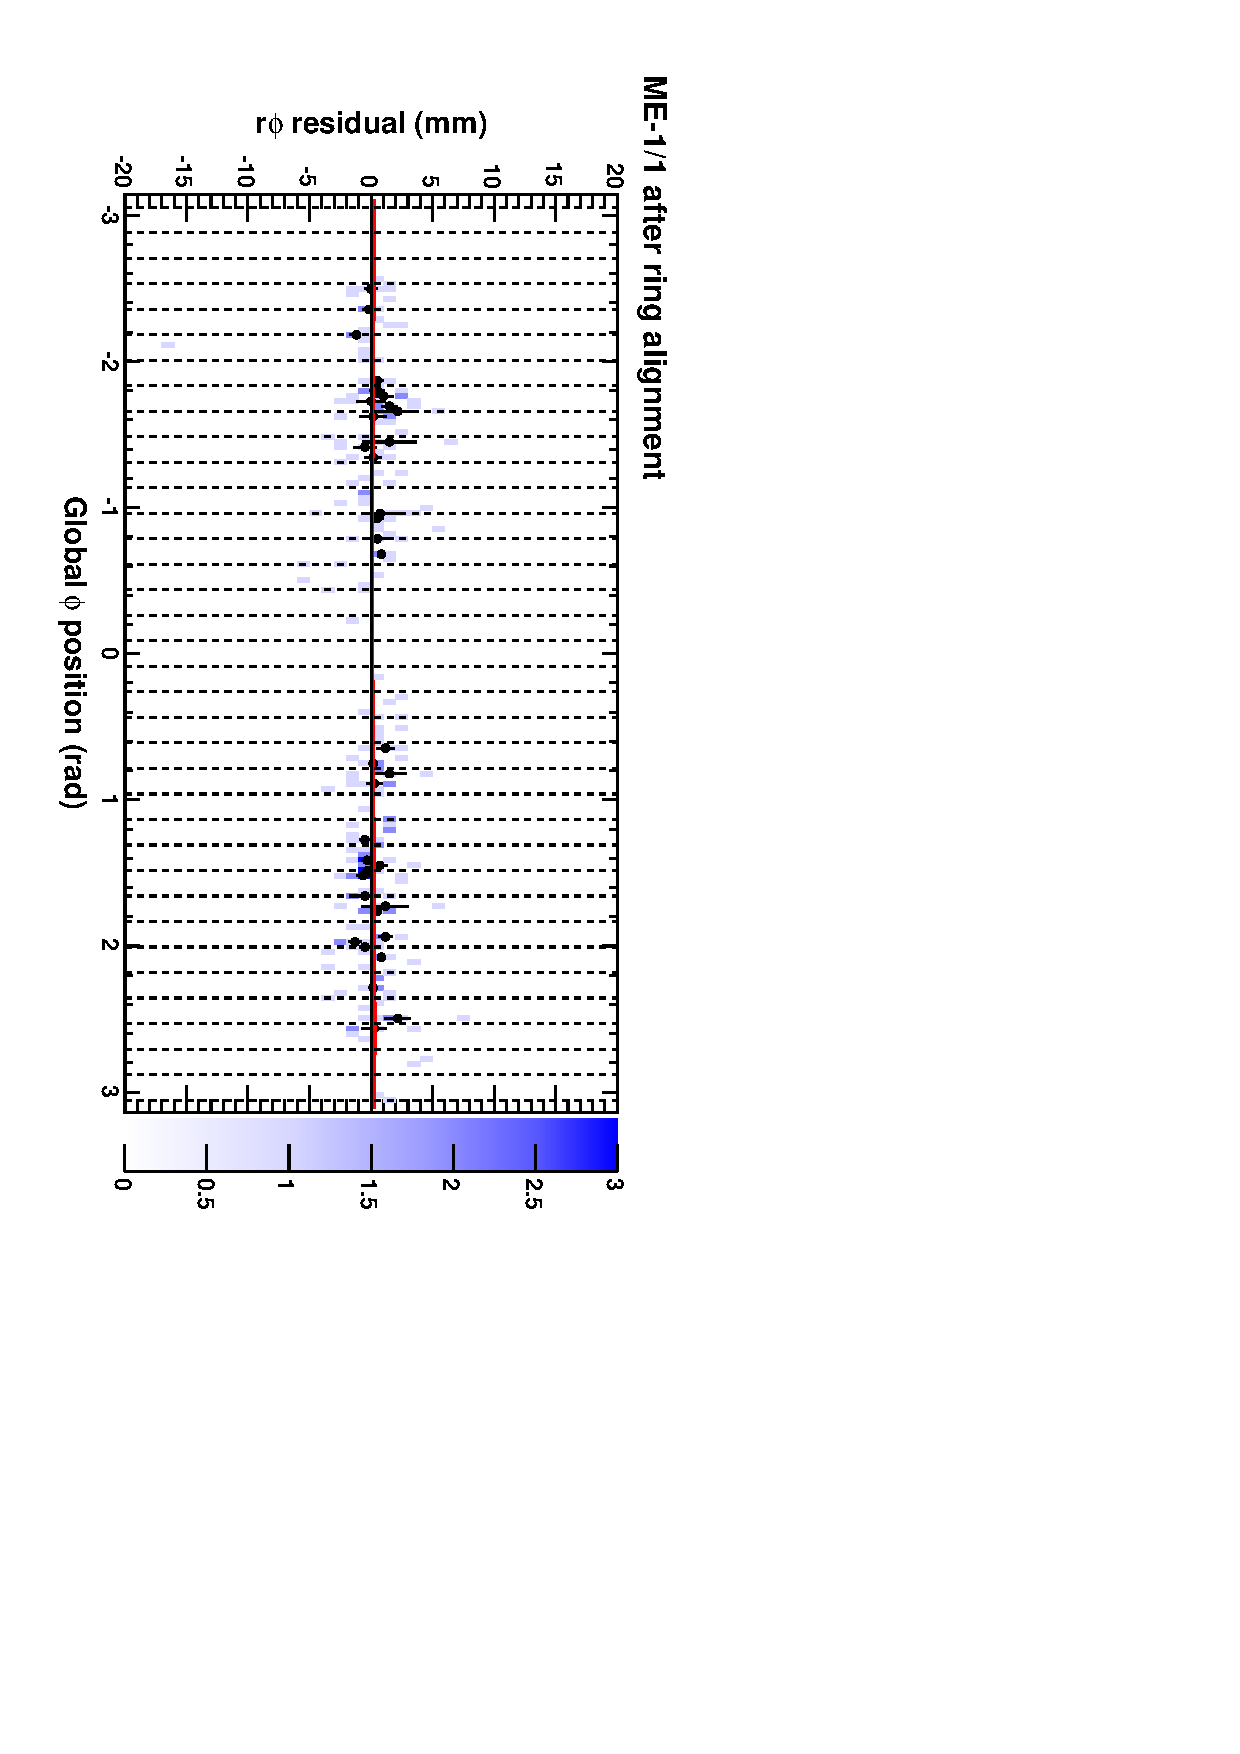
\includegraphics[height=\linewidth, angle=90]{ringfits_after/mem11.pdf}
\column{0.3\linewidth}
\begin{itemize}
\item Unbiased residuals from tracker tracks
\item Color scale is 2-D plot
\item Black points are a profile (averages in vertical bins)
\item Red line is fit to 2-D data
\item sine $\sim$ $X$ \\
cosine $\sim$ $Y$ \\
constant $\sim$ $\phi_Z$
\end{itemize}
\end{columns}
\end{frame}

\begin{frame}
\frametitle{Ring fits: ME$+$1/1}
\vfill
\begin{columns}
\column{0.7\linewidth}
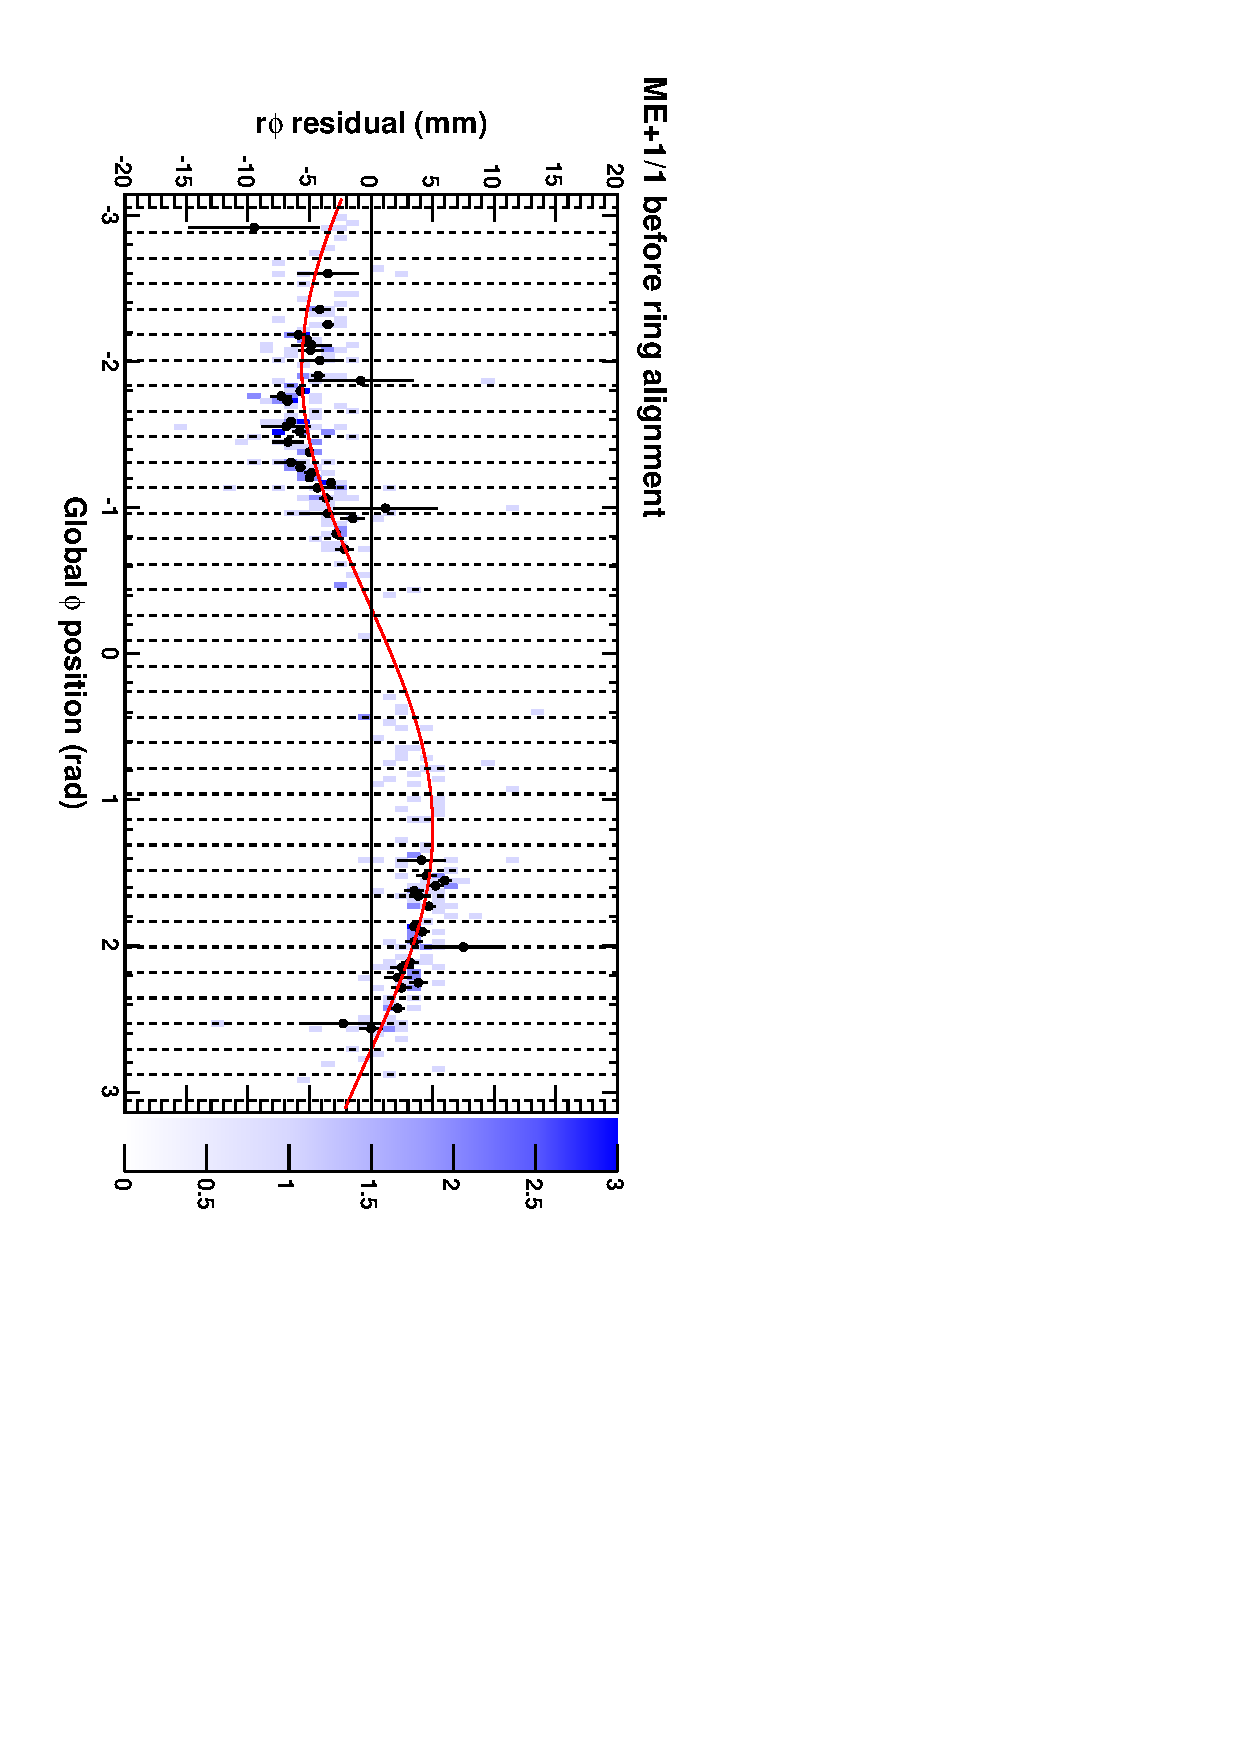
\includegraphics[height=\linewidth, angle=90]{ringfits_before/mep11.pdf}

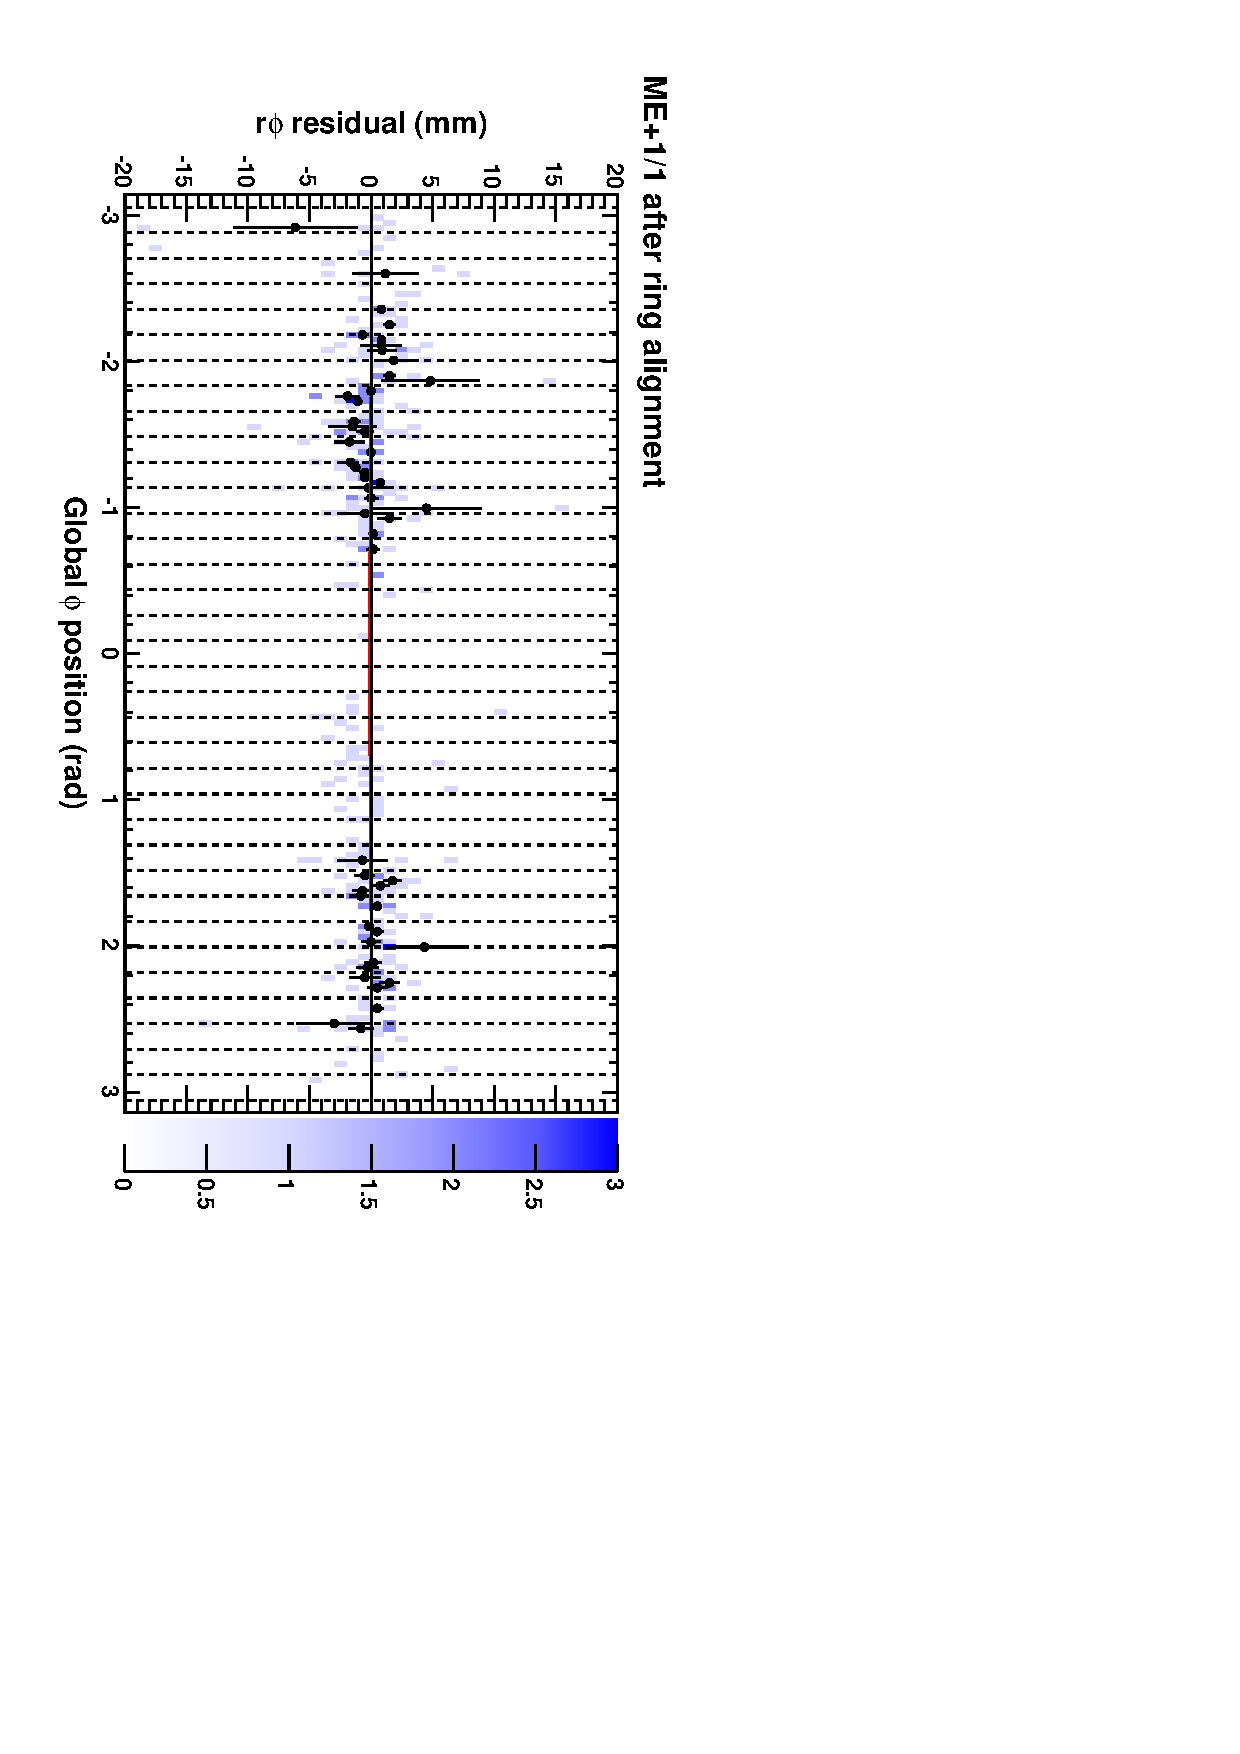
\includegraphics[height=\linewidth, angle=90]{ringfits_after/mep11.pdf}
\column{0.3\linewidth}
\begin{itemize}
\item Unbiased residuals from tracker tracks
\item Color scale is 2-D plot
\item Black points are a profile (averages in vertical bins)
\item Red line is fit to 2-D data
\item sine $\sim$ $X$ \\
cosine $\sim$ $Y$ \\
constant $\sim$ $\phi_Z$
\end{itemize}
\end{columns}
\end{frame}

\begin{frame}
\frametitle{Ring fits: ME$+$1/2}
\vfill
\begin{columns}
\column{0.7\linewidth}
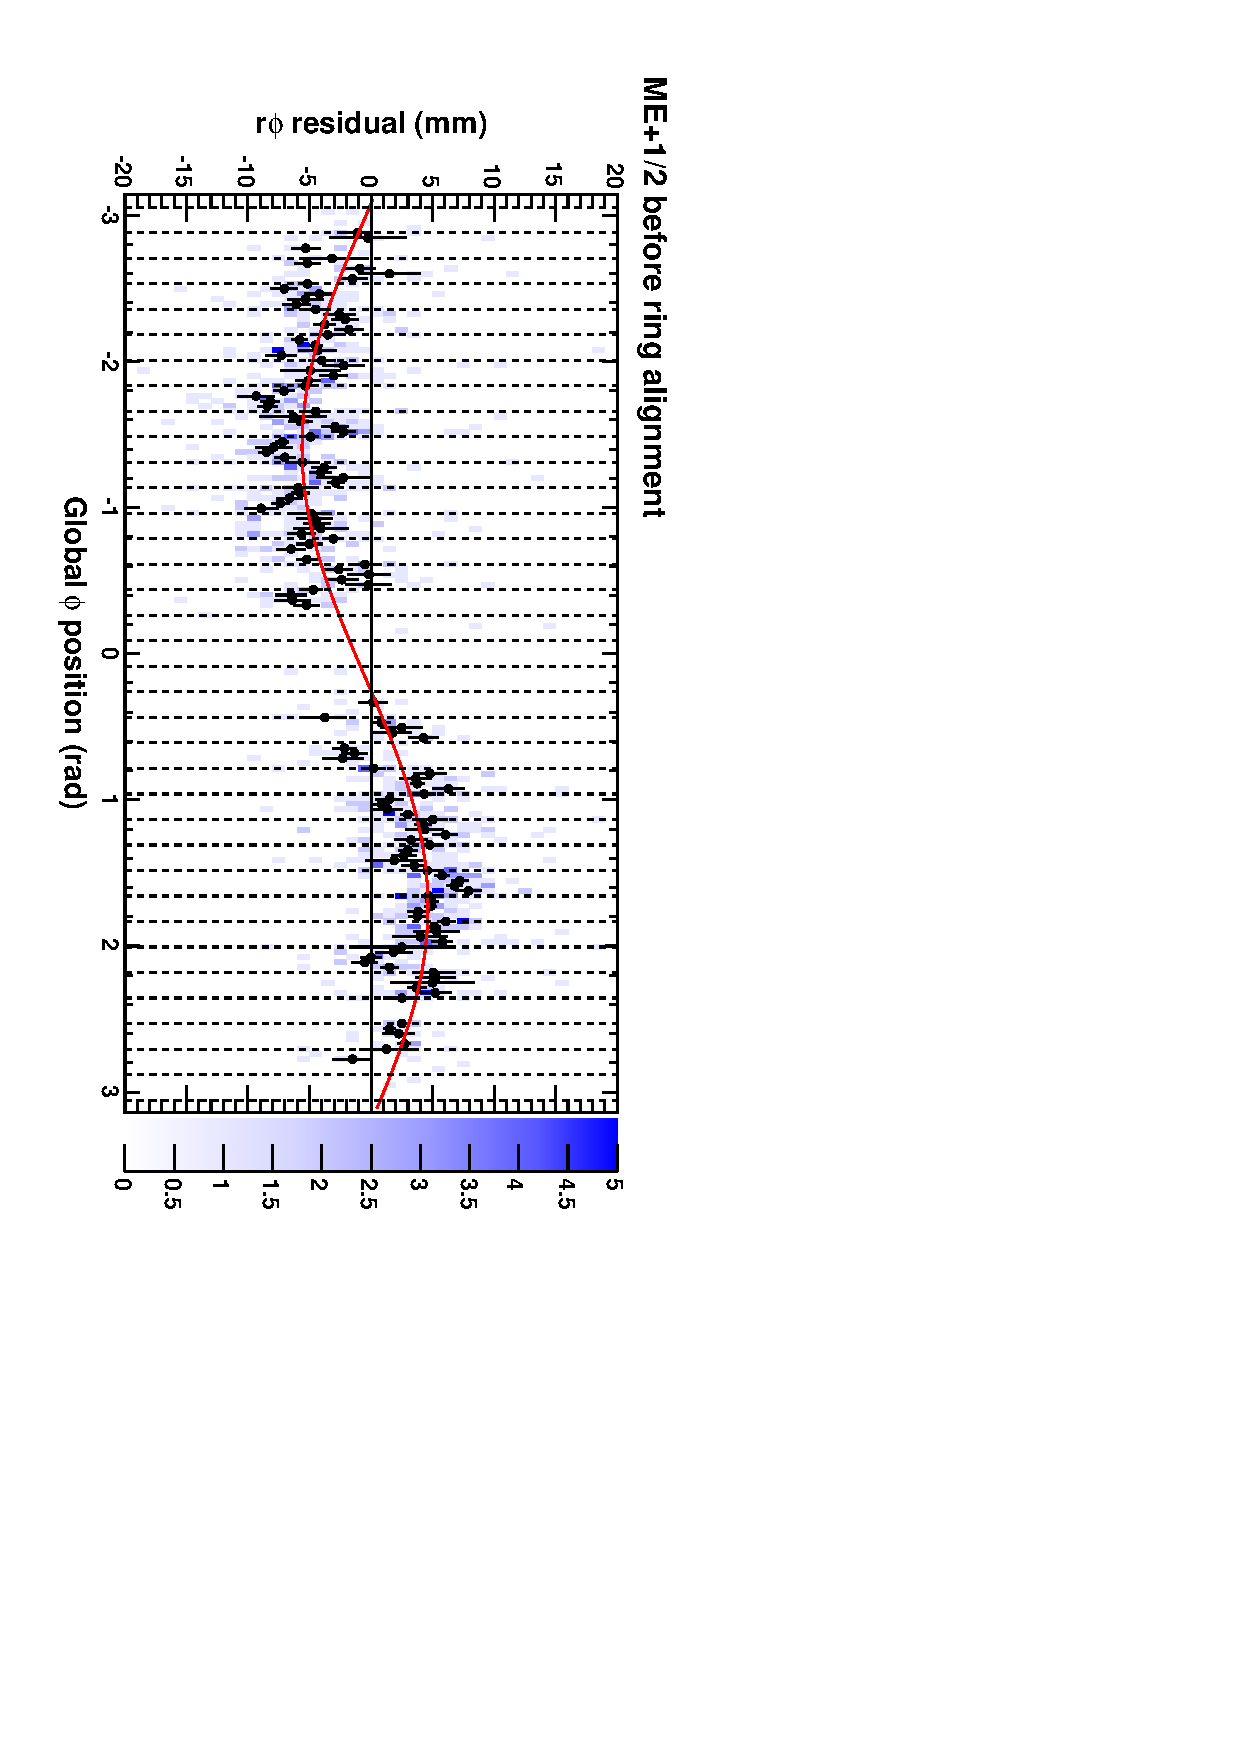
\includegraphics[height=\linewidth, angle=90]{ringfits_before/mep12.pdf}

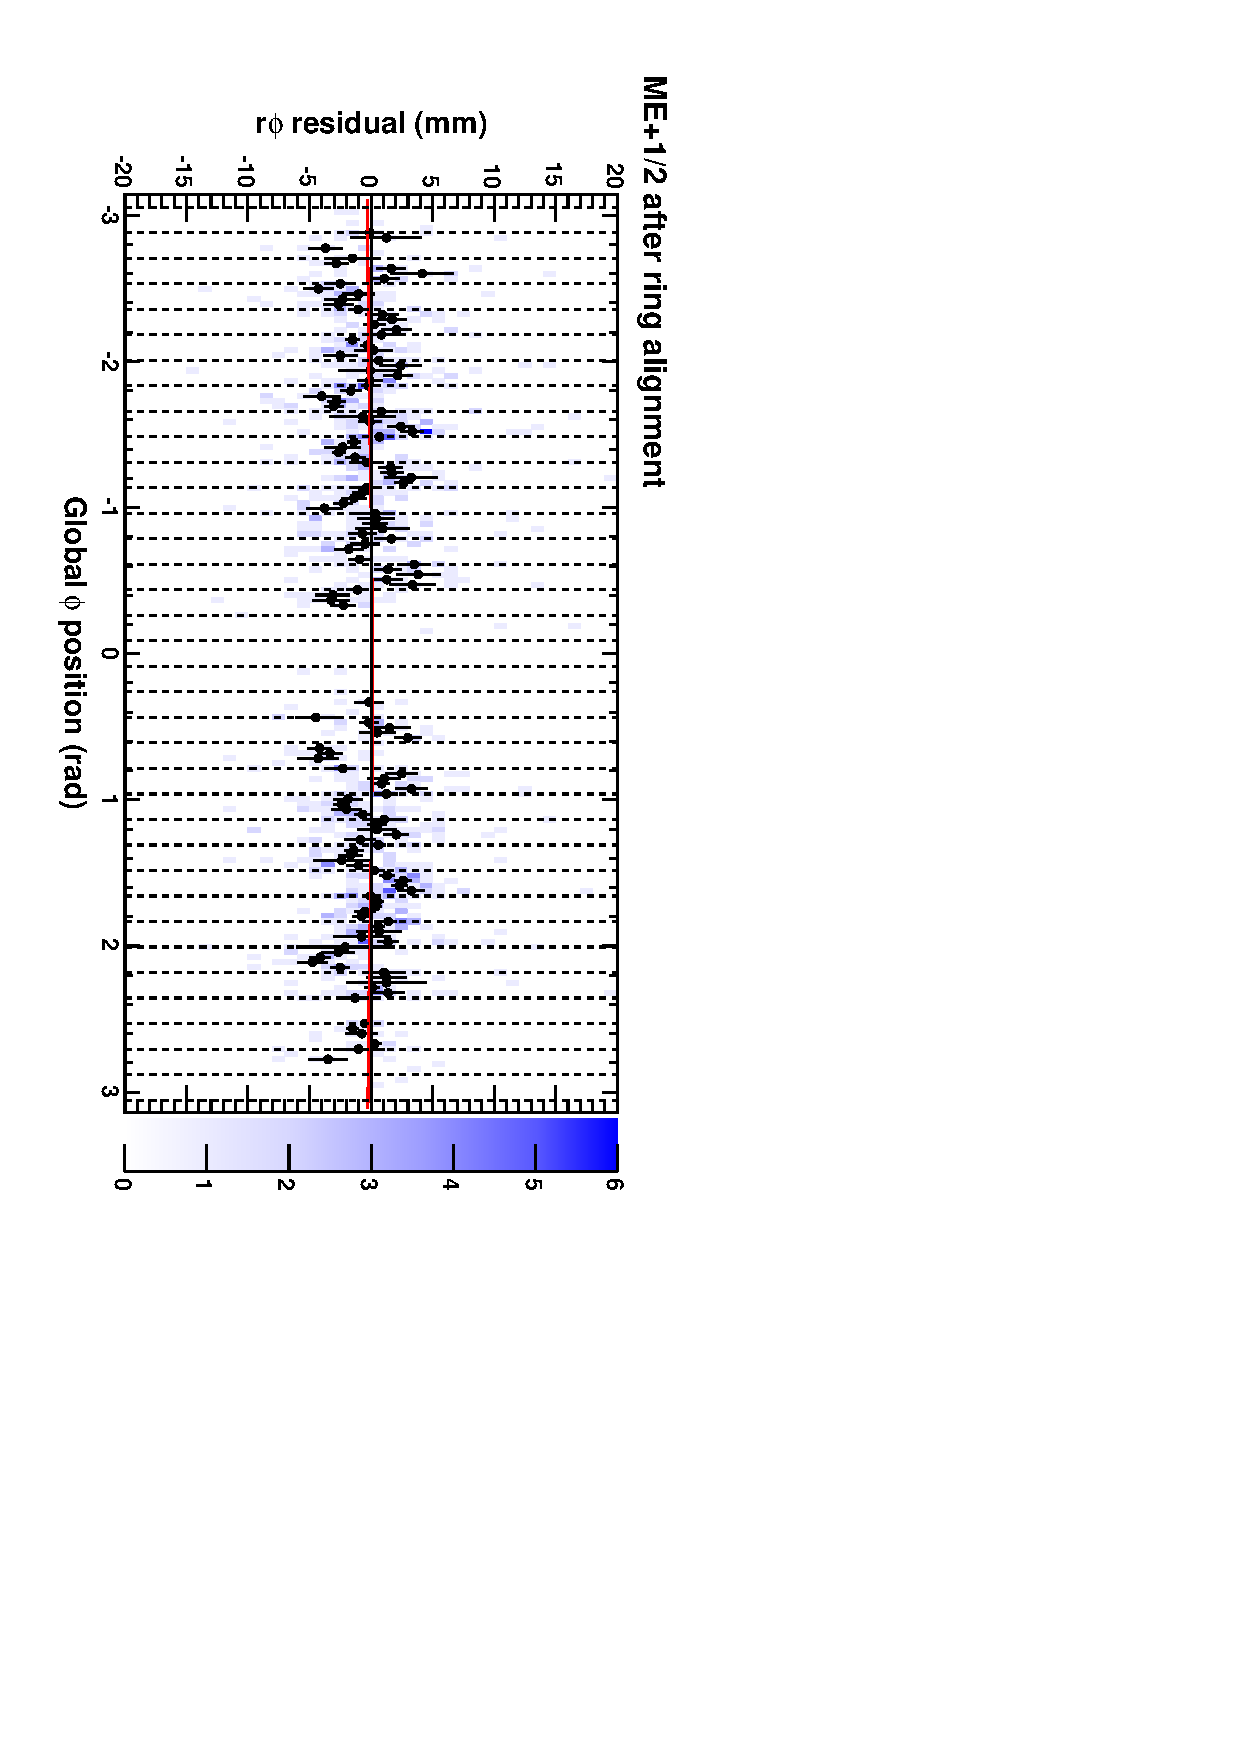
\includegraphics[height=\linewidth, angle=90]{ringfits_after/mep12.pdf}
\column{0.3\linewidth}
\begin{itemize}
\item Unbiased residuals from tracker tracks
\item Color scale is 2-D plot
\item Black points are a profile (averages in vertical bins)
\item Red line is fit to 2-D data
\item sine $\sim$ $X$ \\
cosine $\sim$ $Y$ \\
constant $\sim$ $\phi_Z$
\end{itemize}
\end{columns}
\end{frame}

\begin{frame}
\frametitle{Ring fits: ME$+$1/3}
\vfill
\begin{columns}
\column{0.7\linewidth}
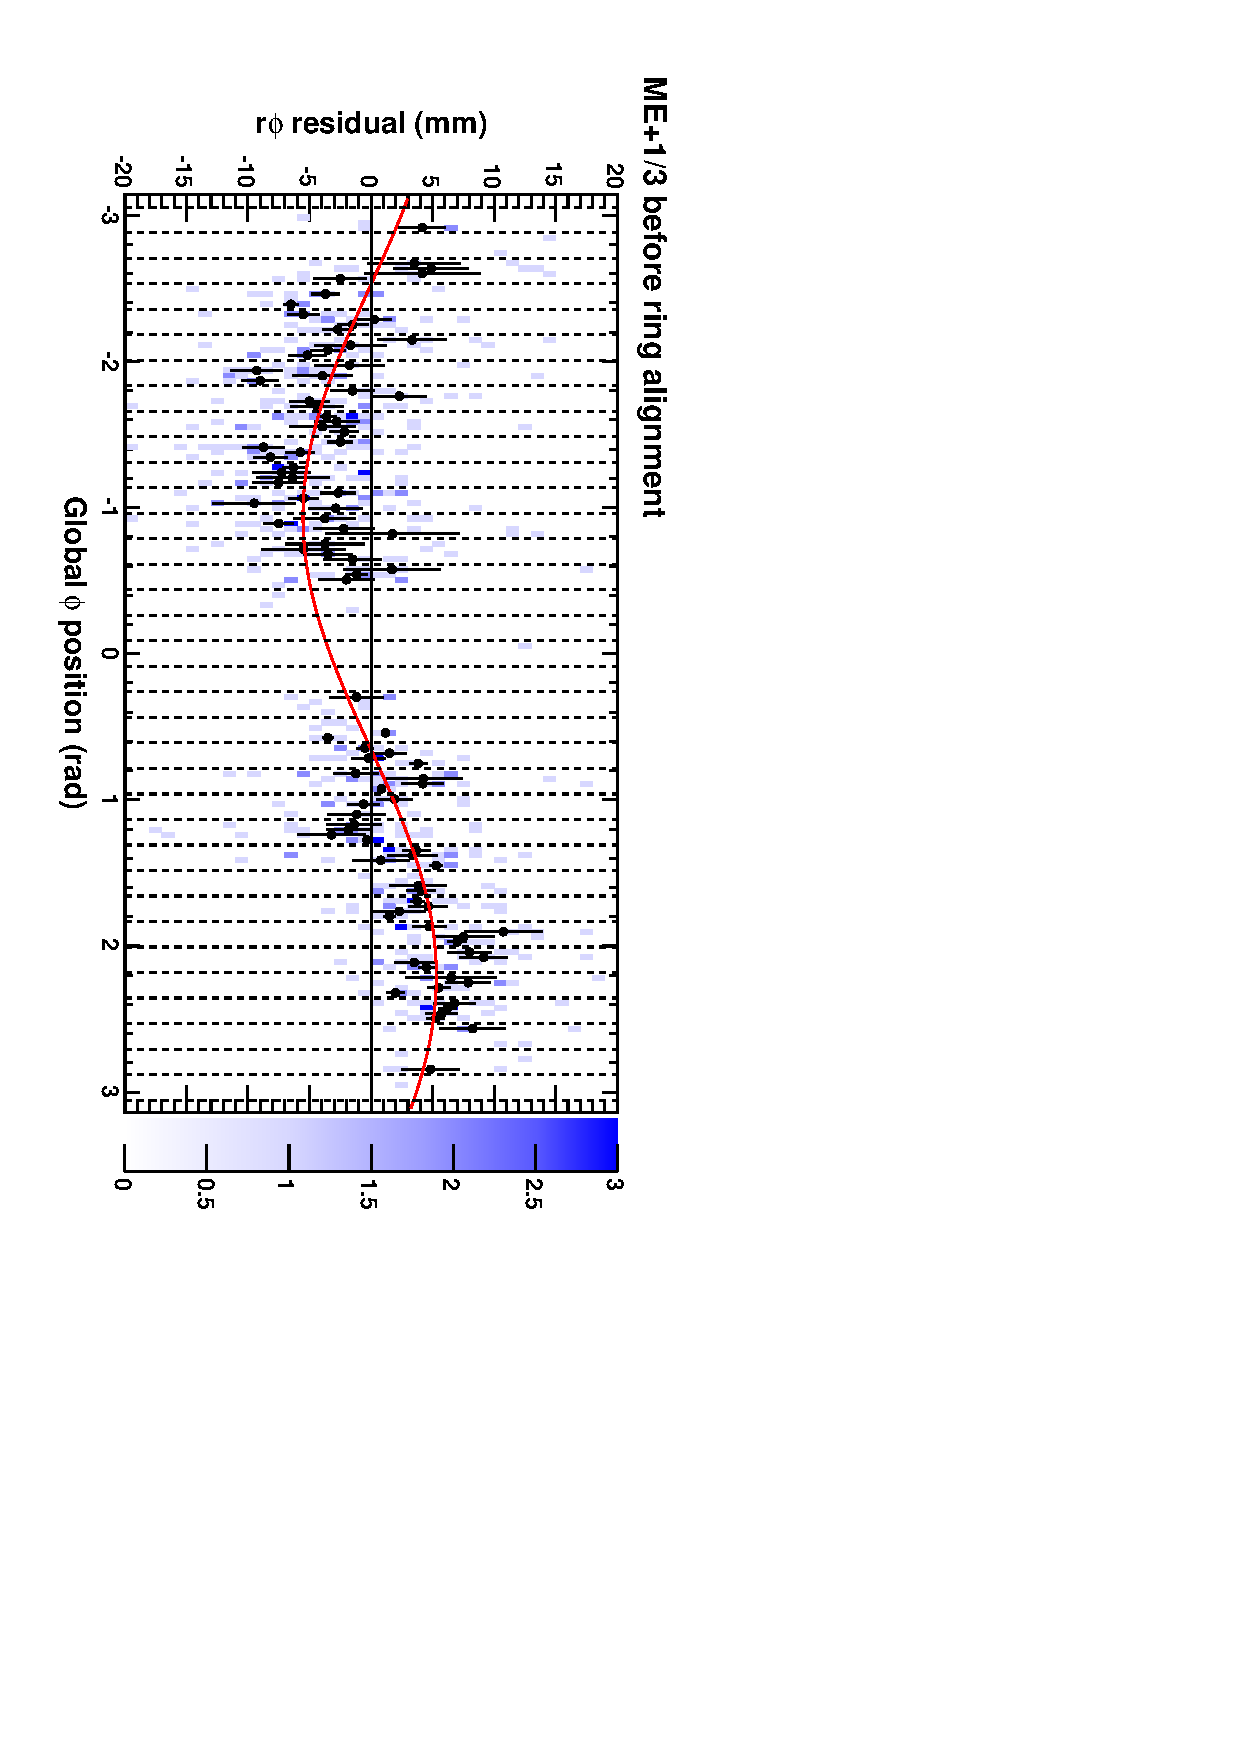
\includegraphics[height=\linewidth, angle=90]{ringfits_before/mep13.pdf}

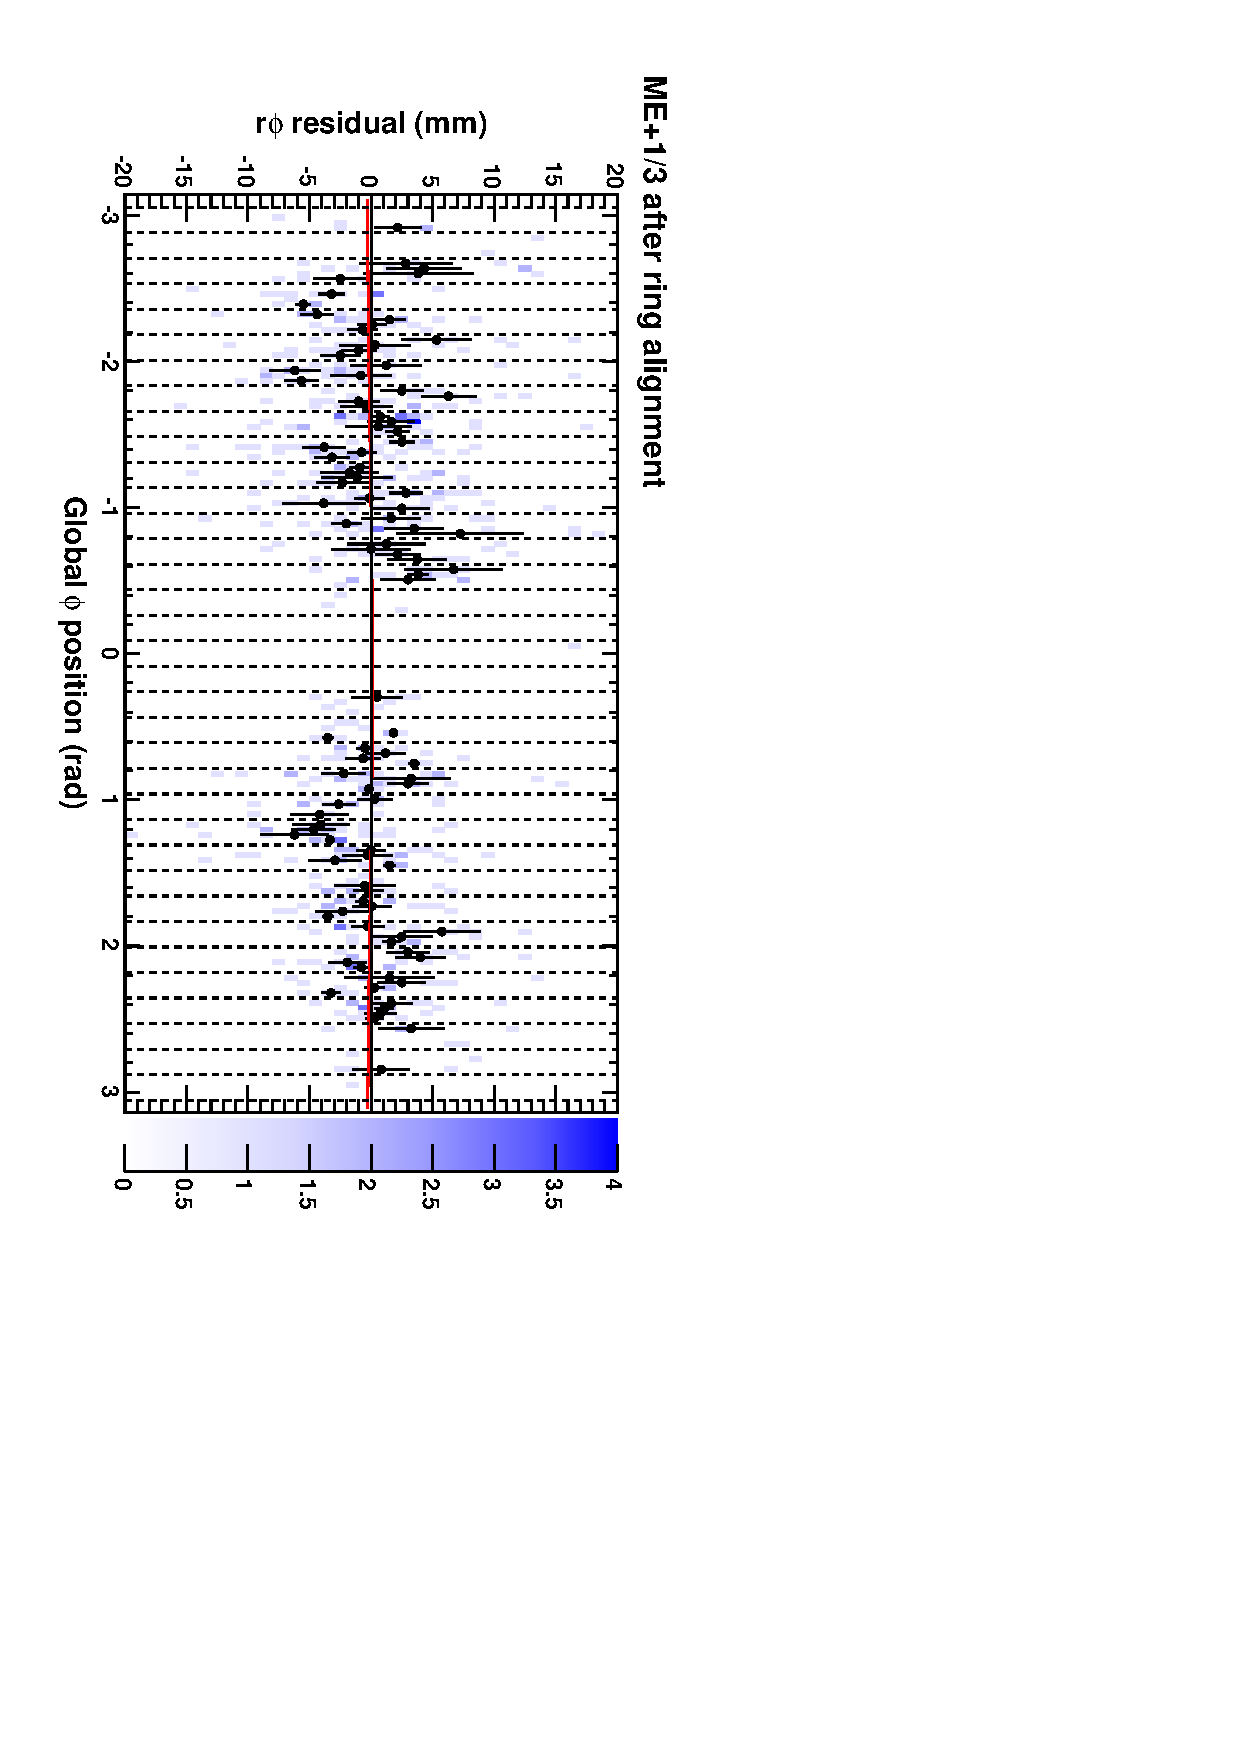
\includegraphics[height=\linewidth, angle=90]{ringfits_after/mep13.pdf}
\column{0.3\linewidth}
\begin{itemize}
\item Unbiased residuals from tracker tracks
\item Color scale is 2-D plot
\item Black points are a profile (averages in vertical bins)
\item Red line is fit to 2-D data
\item sine $\sim$ $X$ \\
cosine $\sim$ $Y$ \\
constant $\sim$ $\phi_Z$
\end{itemize}
\end{columns}
\end{frame}

\begin{frame}
\frametitle{Ring fits: ME$+$2/1}
\vfill
\begin{columns}
\column{0.7\linewidth}
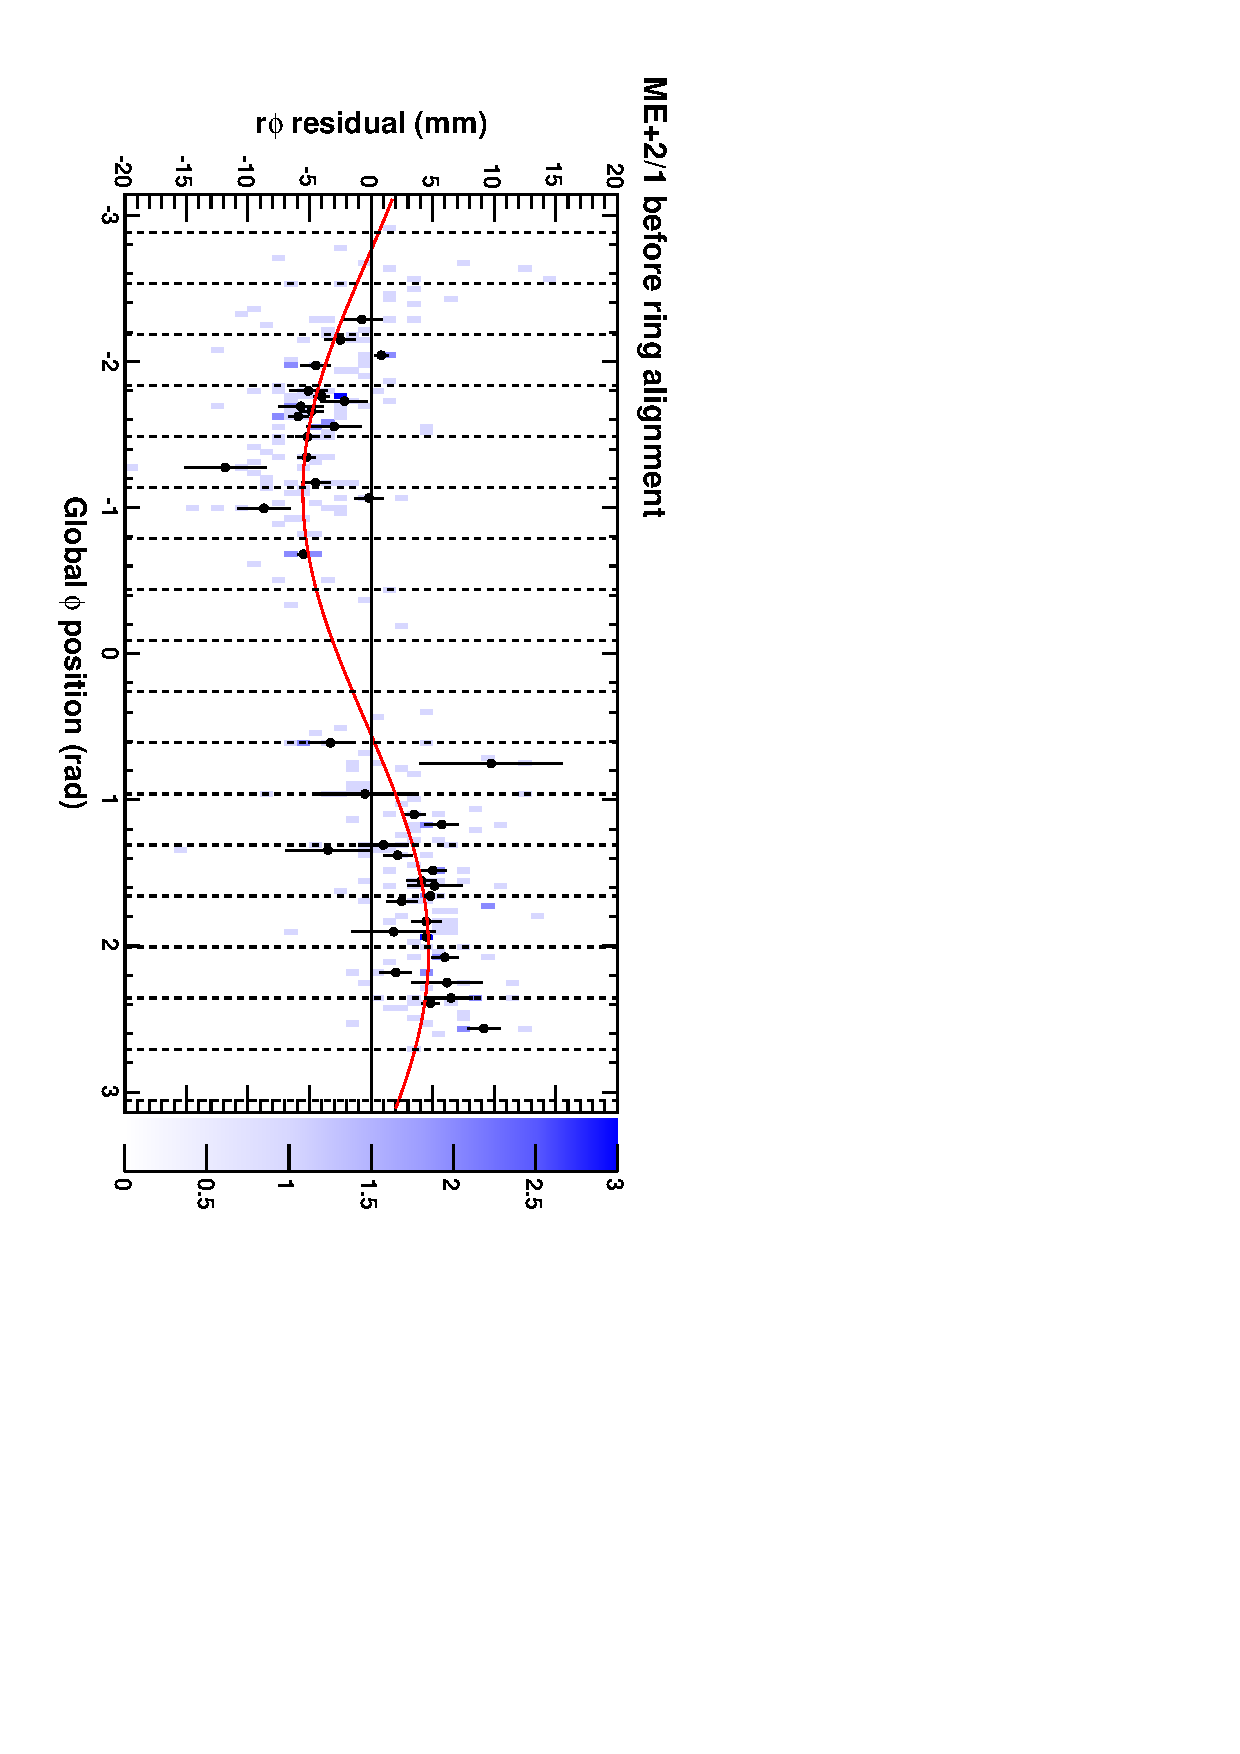
\includegraphics[height=\linewidth, angle=90]{ringfits_before/mep21.pdf}

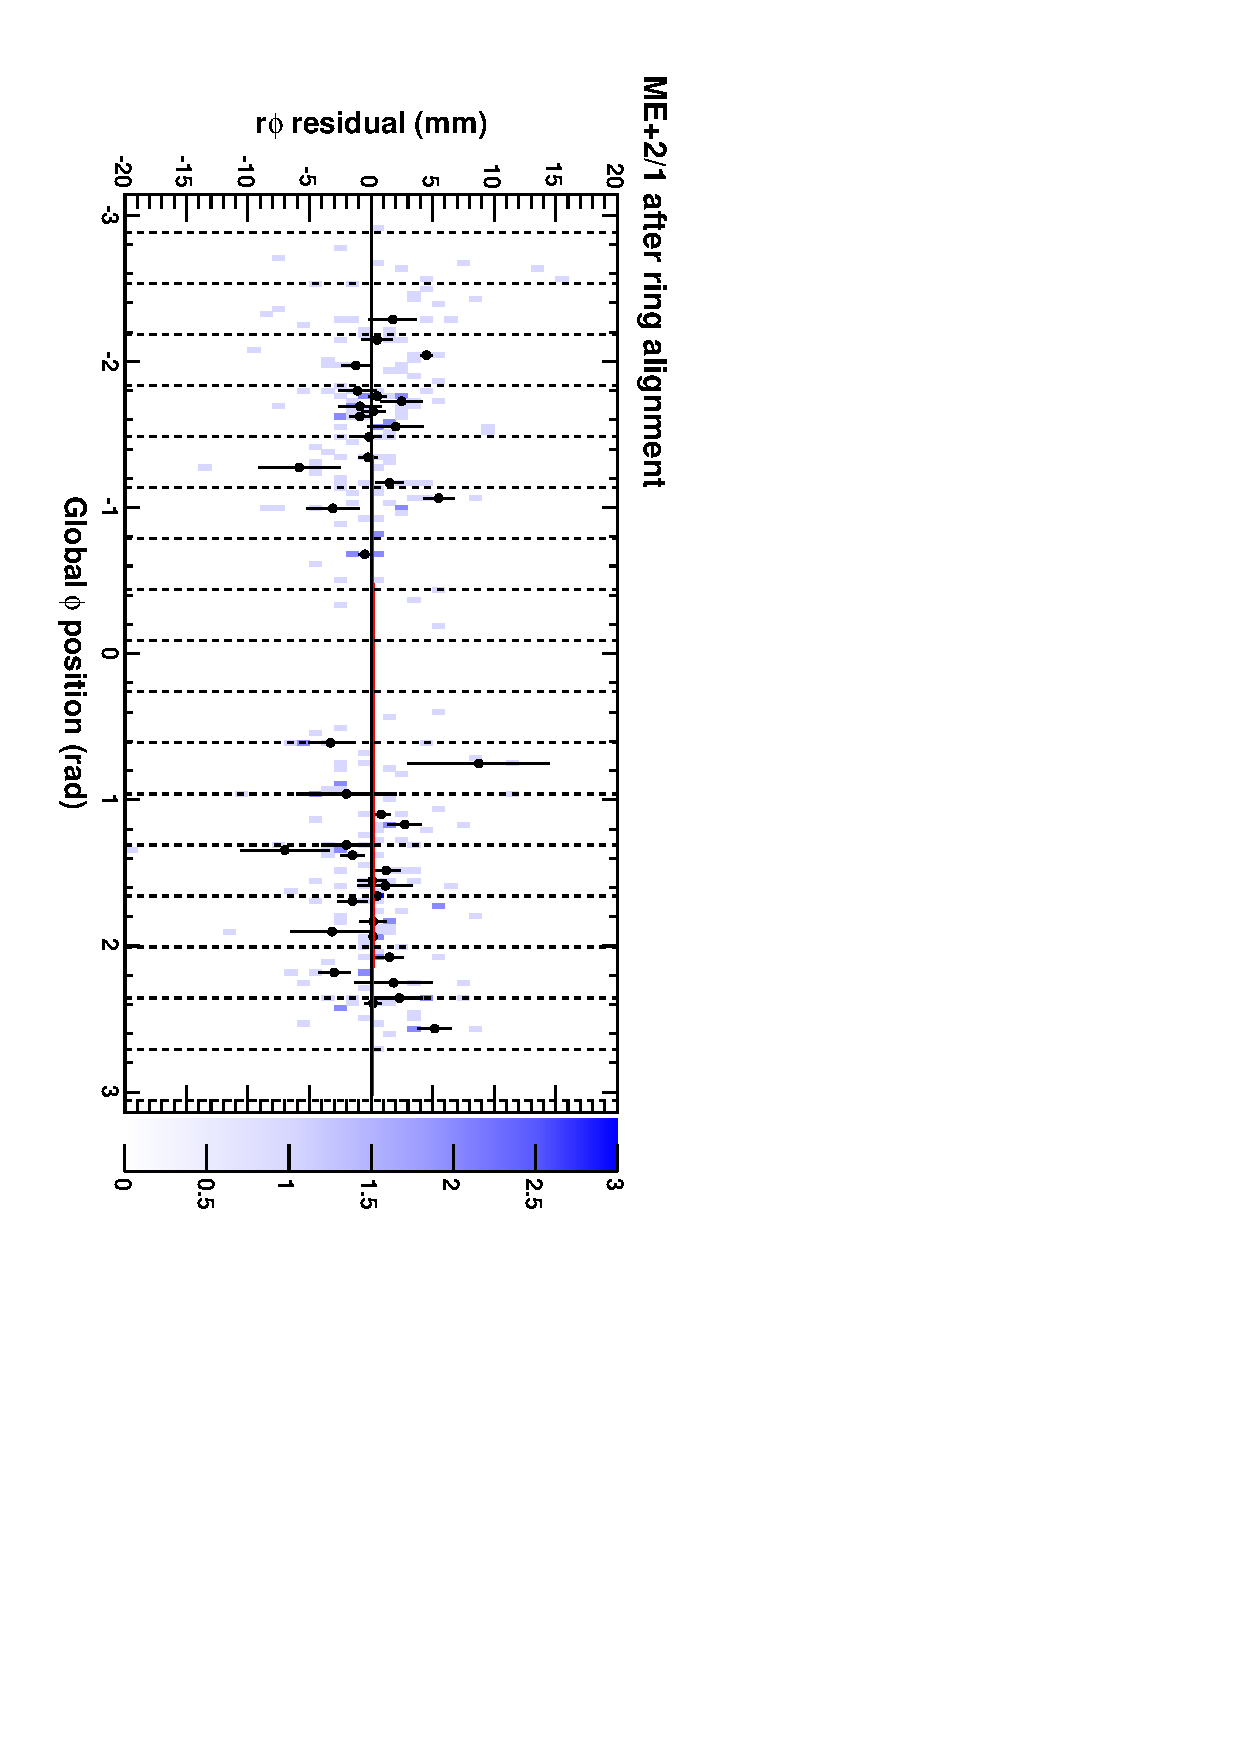
\includegraphics[height=\linewidth, angle=90]{ringfits_after/mep21.pdf}
\column{0.3\linewidth}
\begin{itemize}
\item Unbiased residuals from tracker tracks
\item Color scale is 2-D plot
\item Black points are a profile (averages in vertical bins)
\item Red line is fit to 2-D data
\item sine $\sim$ $X$ \\
cosine $\sim$ $Y$ \\
constant $\sim$ $\phi_Z$
\end{itemize}
\end{columns}
\end{frame}

\begin{frame}
\frametitle{Ring fits: ME$+$2/2}
\vfill
\begin{columns}
\column{0.7\linewidth}
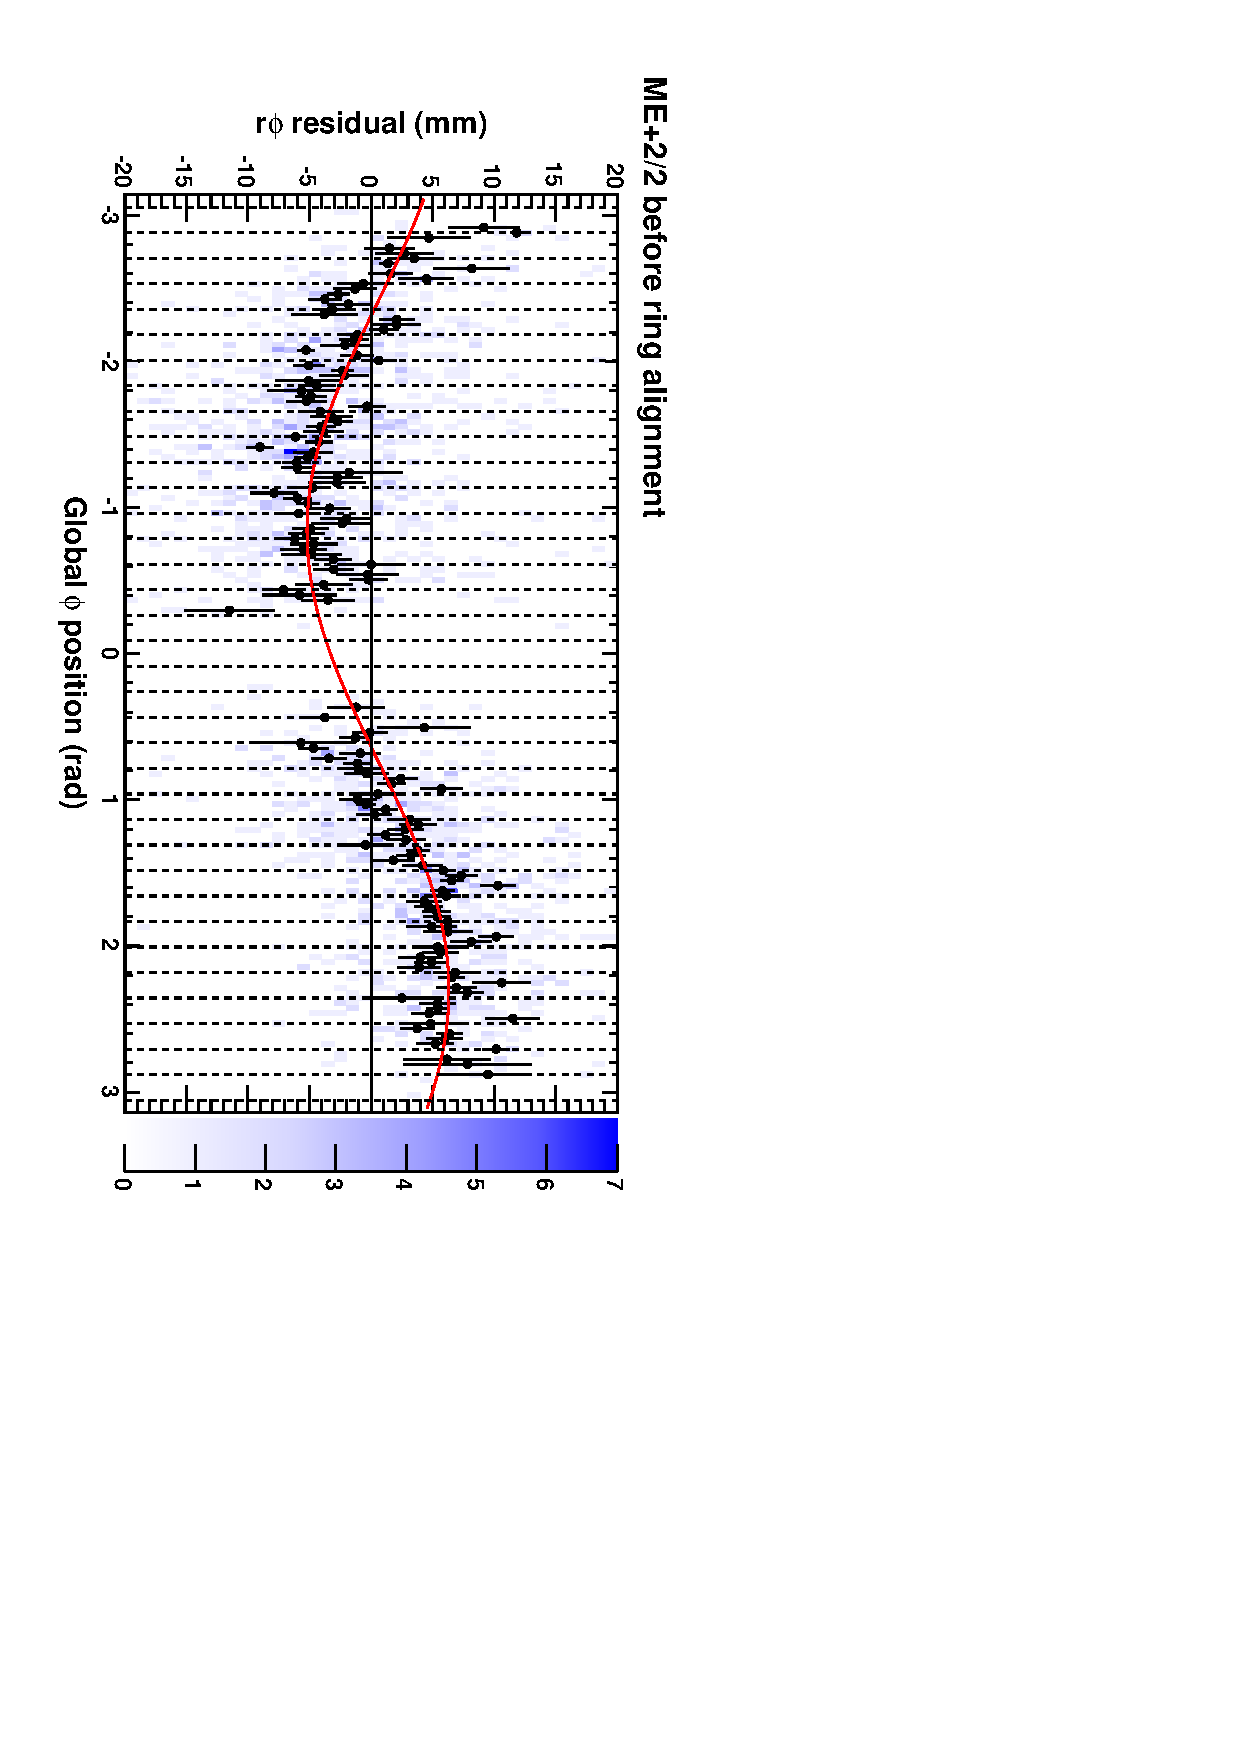
\includegraphics[height=\linewidth, angle=90]{ringfits_before/mep22.pdf}

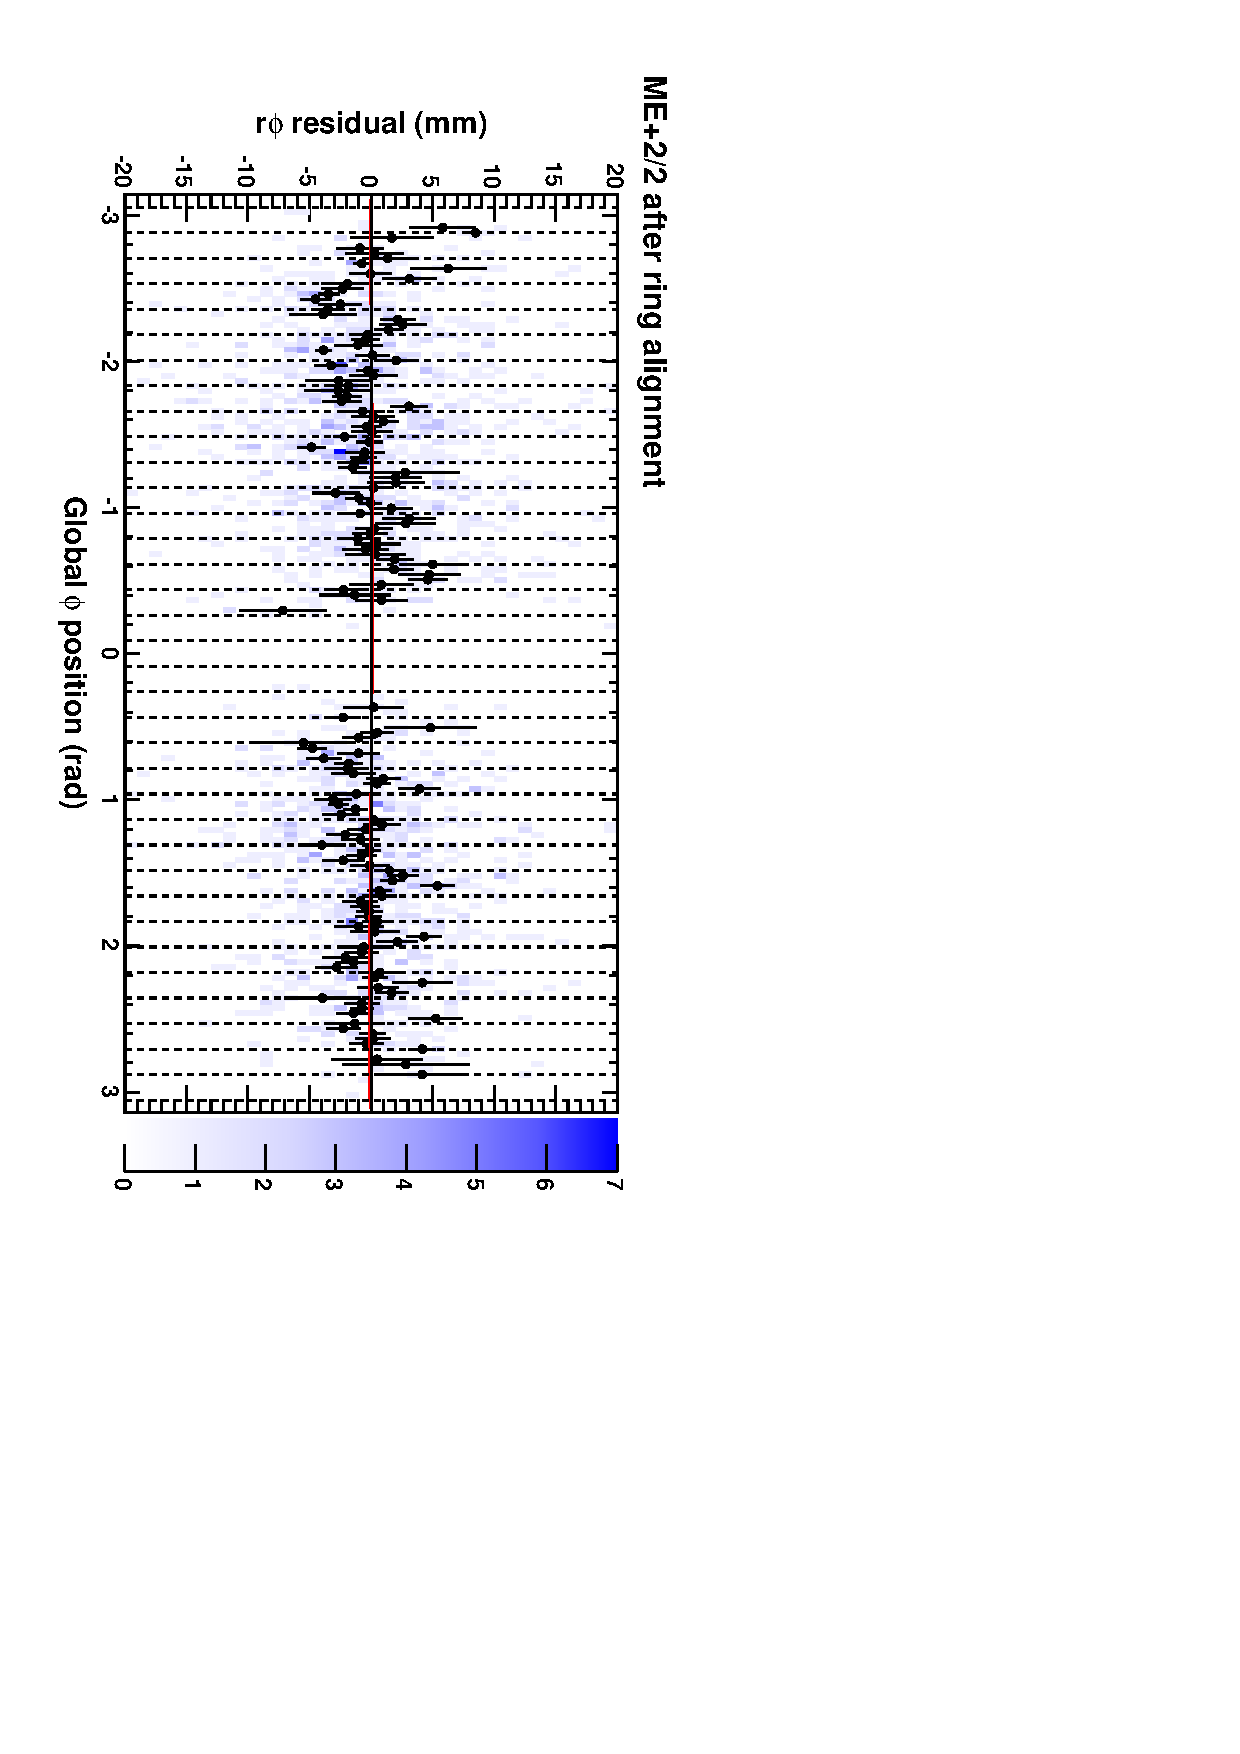
\includegraphics[height=\linewidth, angle=90]{ringfits_after/mep22.pdf}
\column{0.3\linewidth}
\begin{itemize}
\item Unbiased residuals from tracker tracks
\item Color scale is 2-D plot
\item Black points are a profile (averages in vertical bins)
\item Red line is fit to 2-D data
\item sine $\sim$ $X$ \\
cosine $\sim$ $Y$ \\
constant $\sim$ $\phi_Z$
\end{itemize}
\end{columns}
\end{frame}

\begin{frame}
\frametitle{Ring fits: ME$+$3/1}
\vfill
\begin{columns}
\column{0.7\linewidth}
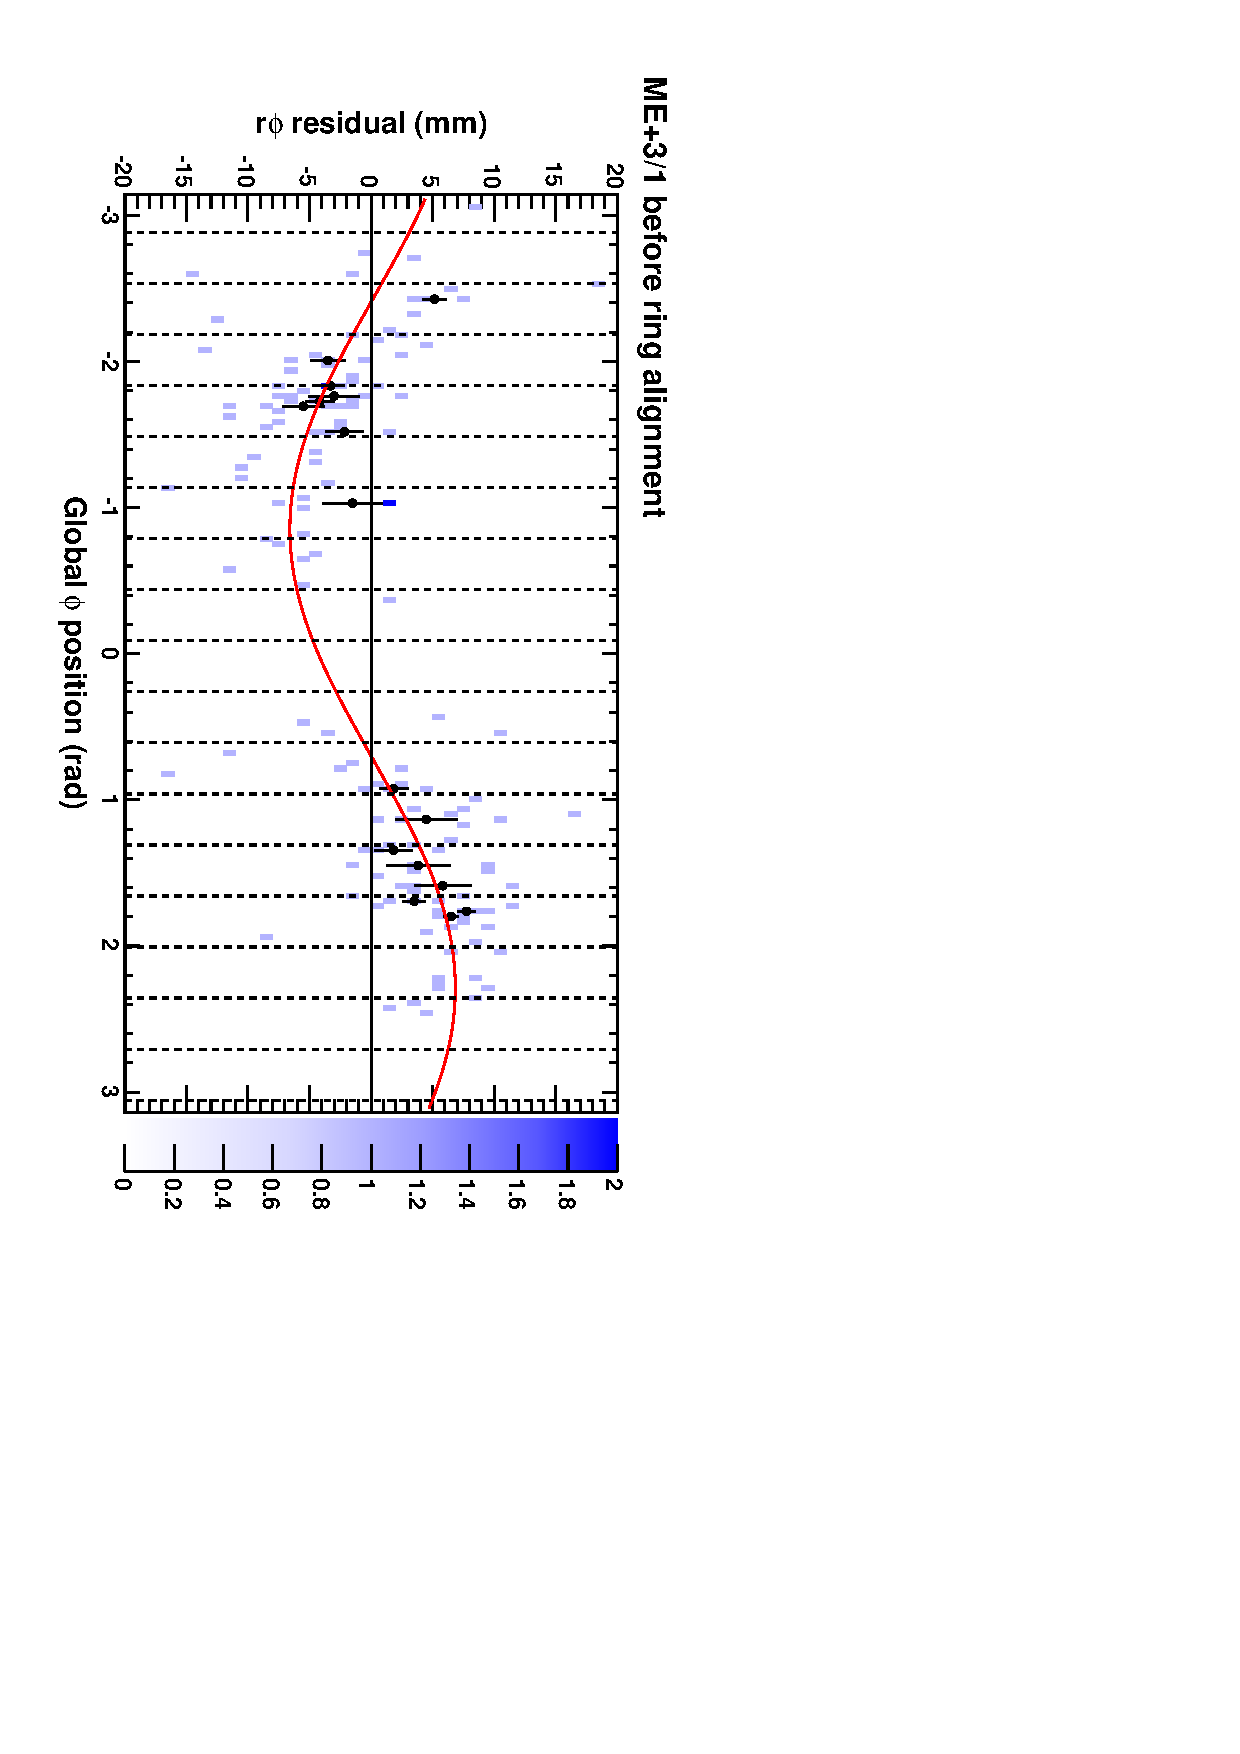
\includegraphics[height=\linewidth, angle=90]{ringfits_before/mep31.pdf}

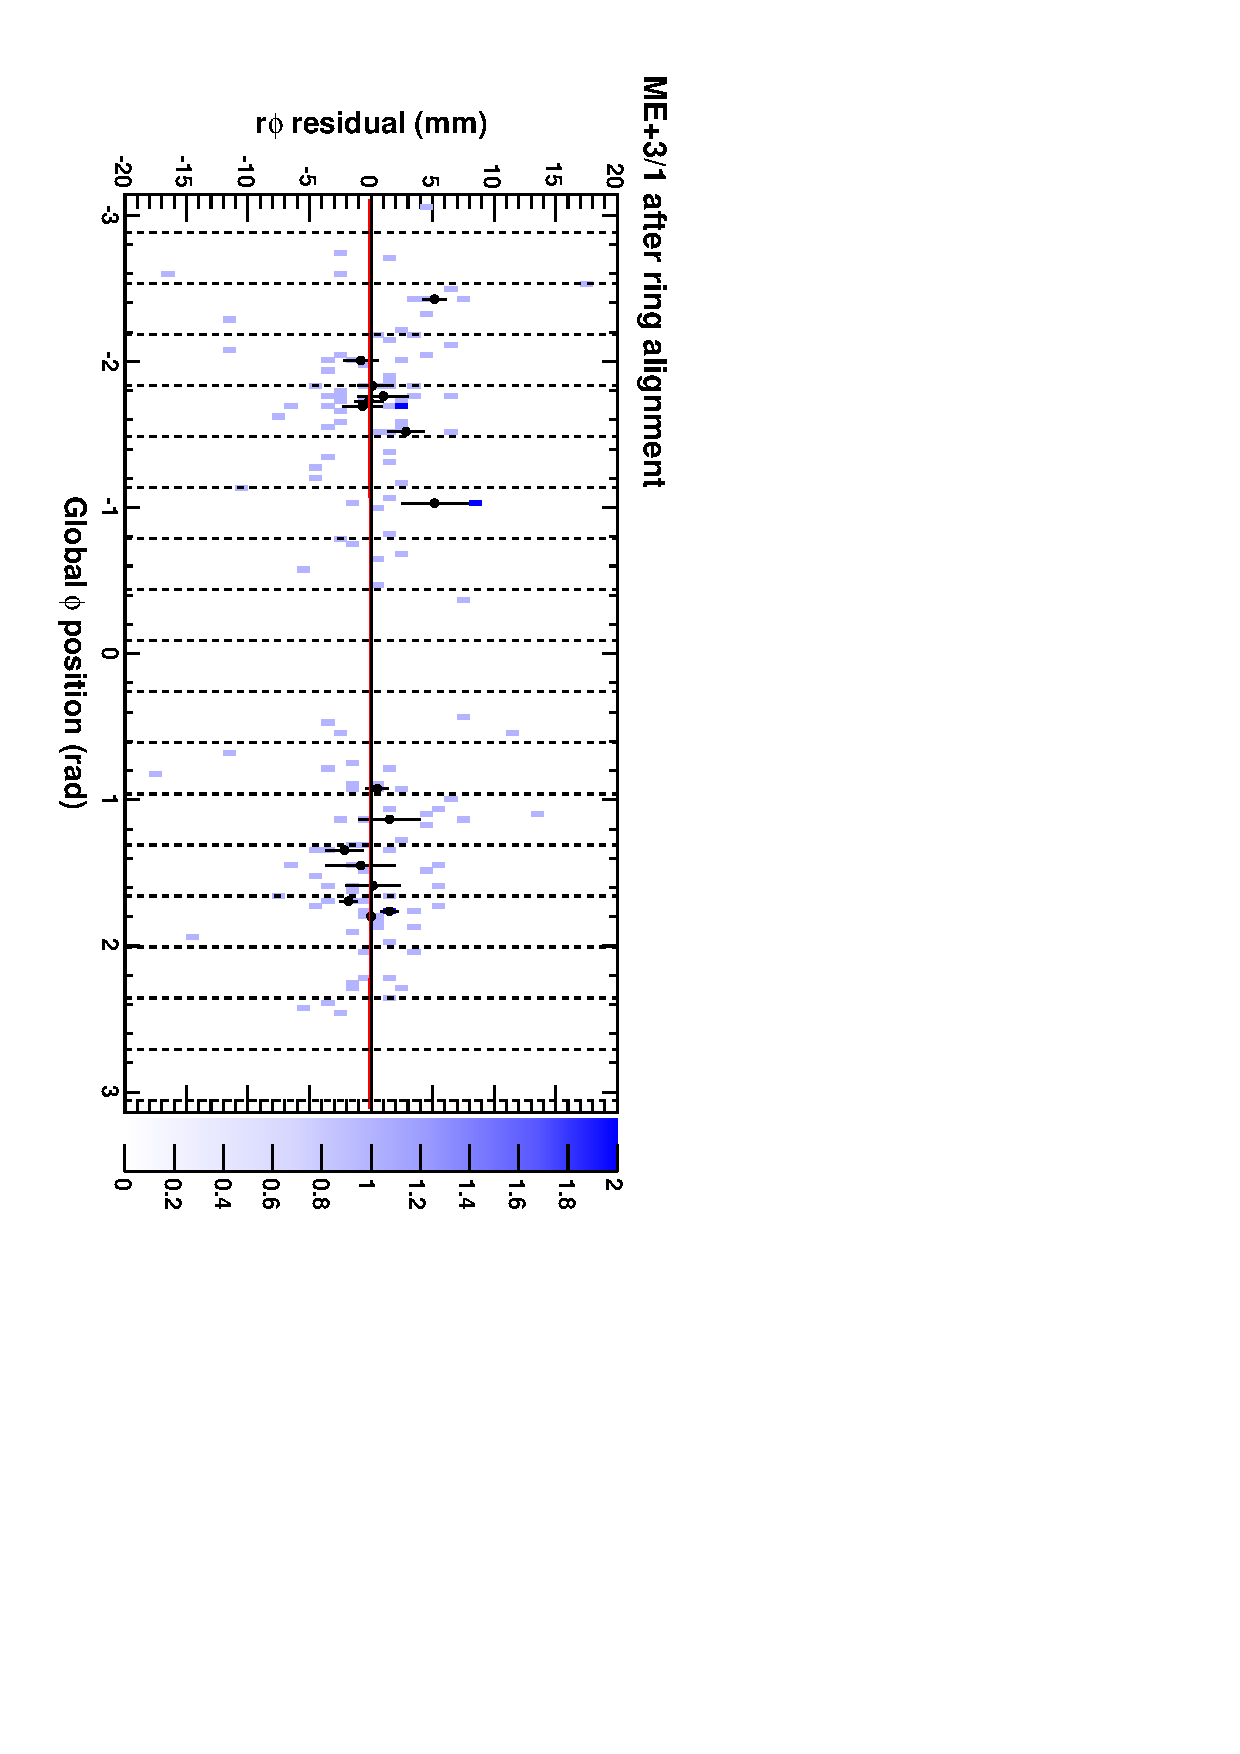
\includegraphics[height=\linewidth, angle=90]{ringfits_after/mep31.pdf}
\column{0.3\linewidth}
\begin{itemize}
\item Unbiased residuals from tracker tracks
\item Color scale is 2-D plot
\item Black points are a profile (averages in vertical bins)
\item Red line is fit to 2-D data
\item sine $\sim$ $X$ \\
cosine $\sim$ $Y$ \\
constant $\sim$ $\phi_Z$
\end{itemize}
\end{columns}
\end{frame}

\begin{frame}
\frametitle{Ring fits: ME$+$3/2}
\vfill
\begin{columns}
\column{0.7\linewidth}
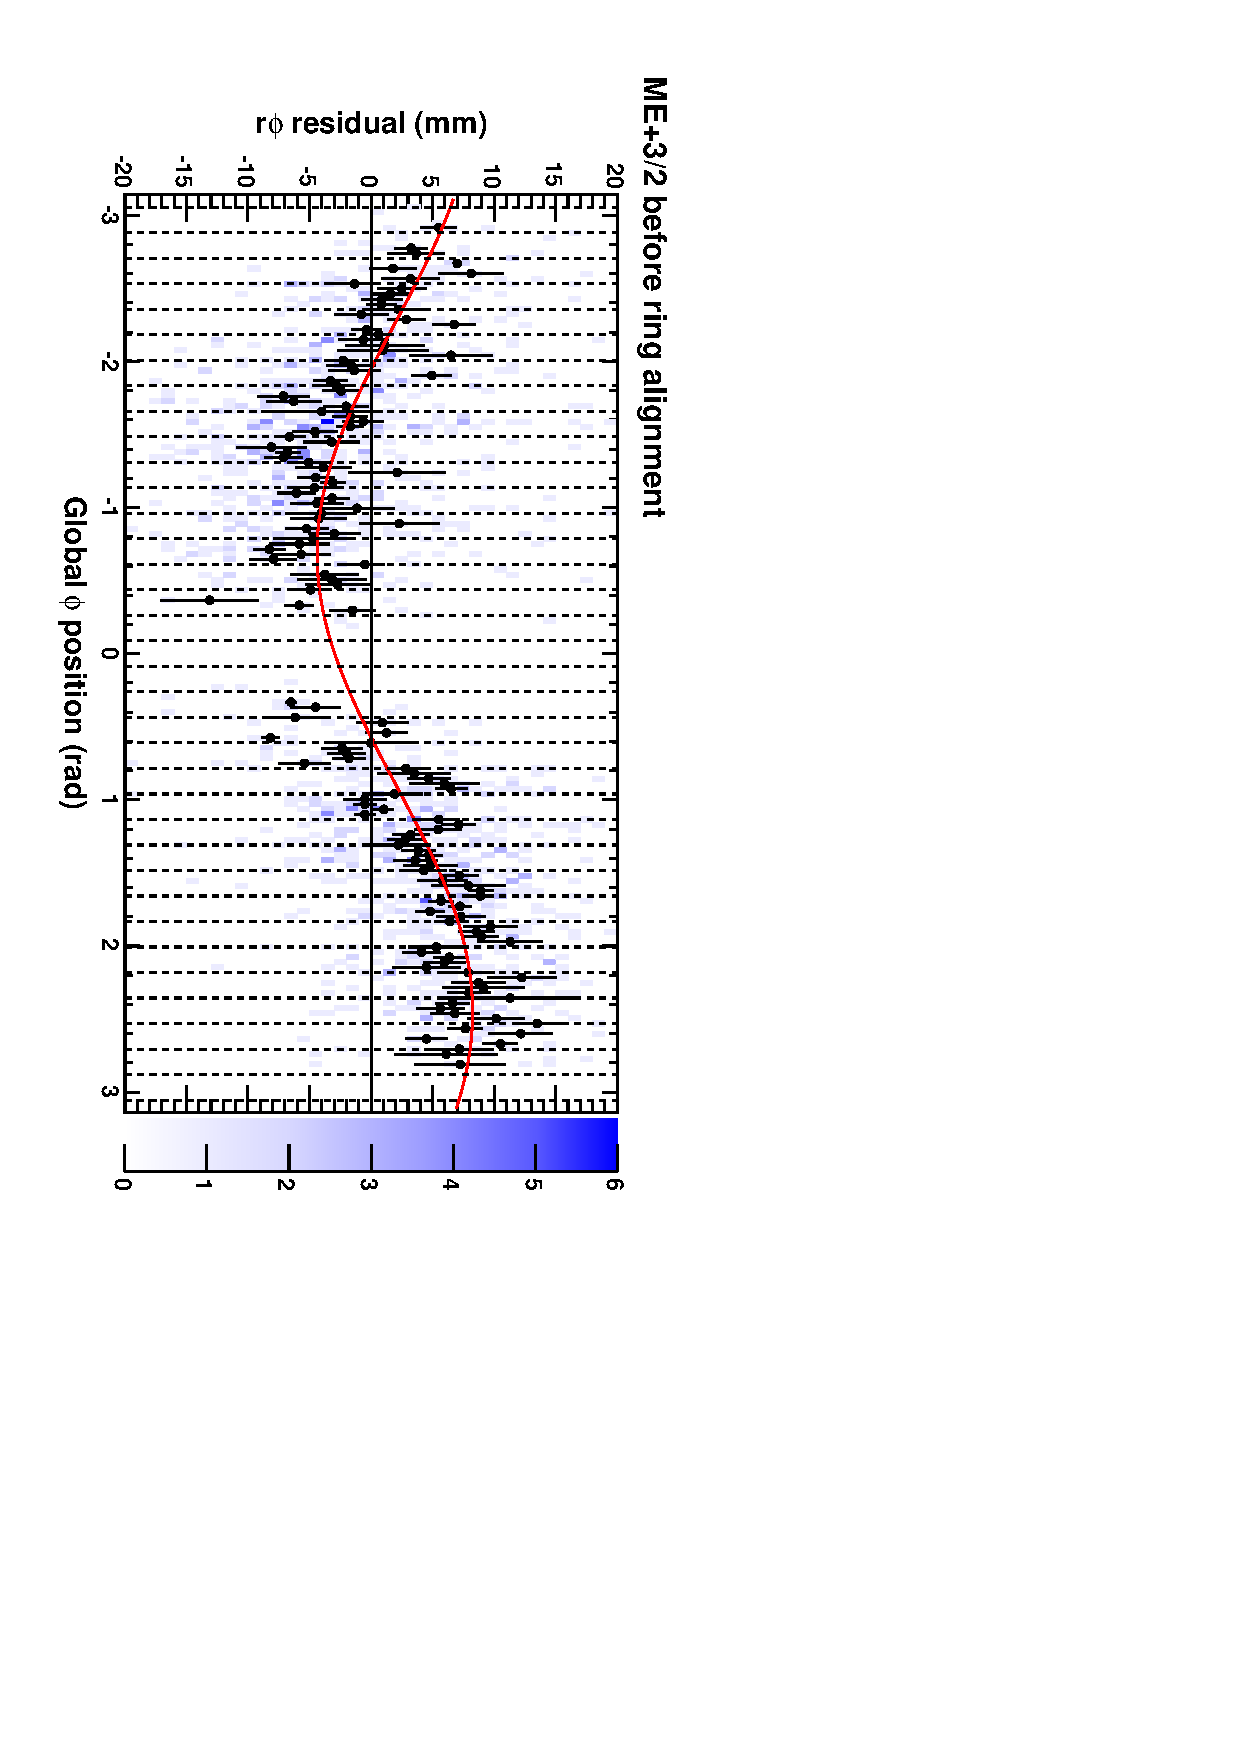
\includegraphics[height=\linewidth, angle=90]{ringfits_before/mep32.pdf}

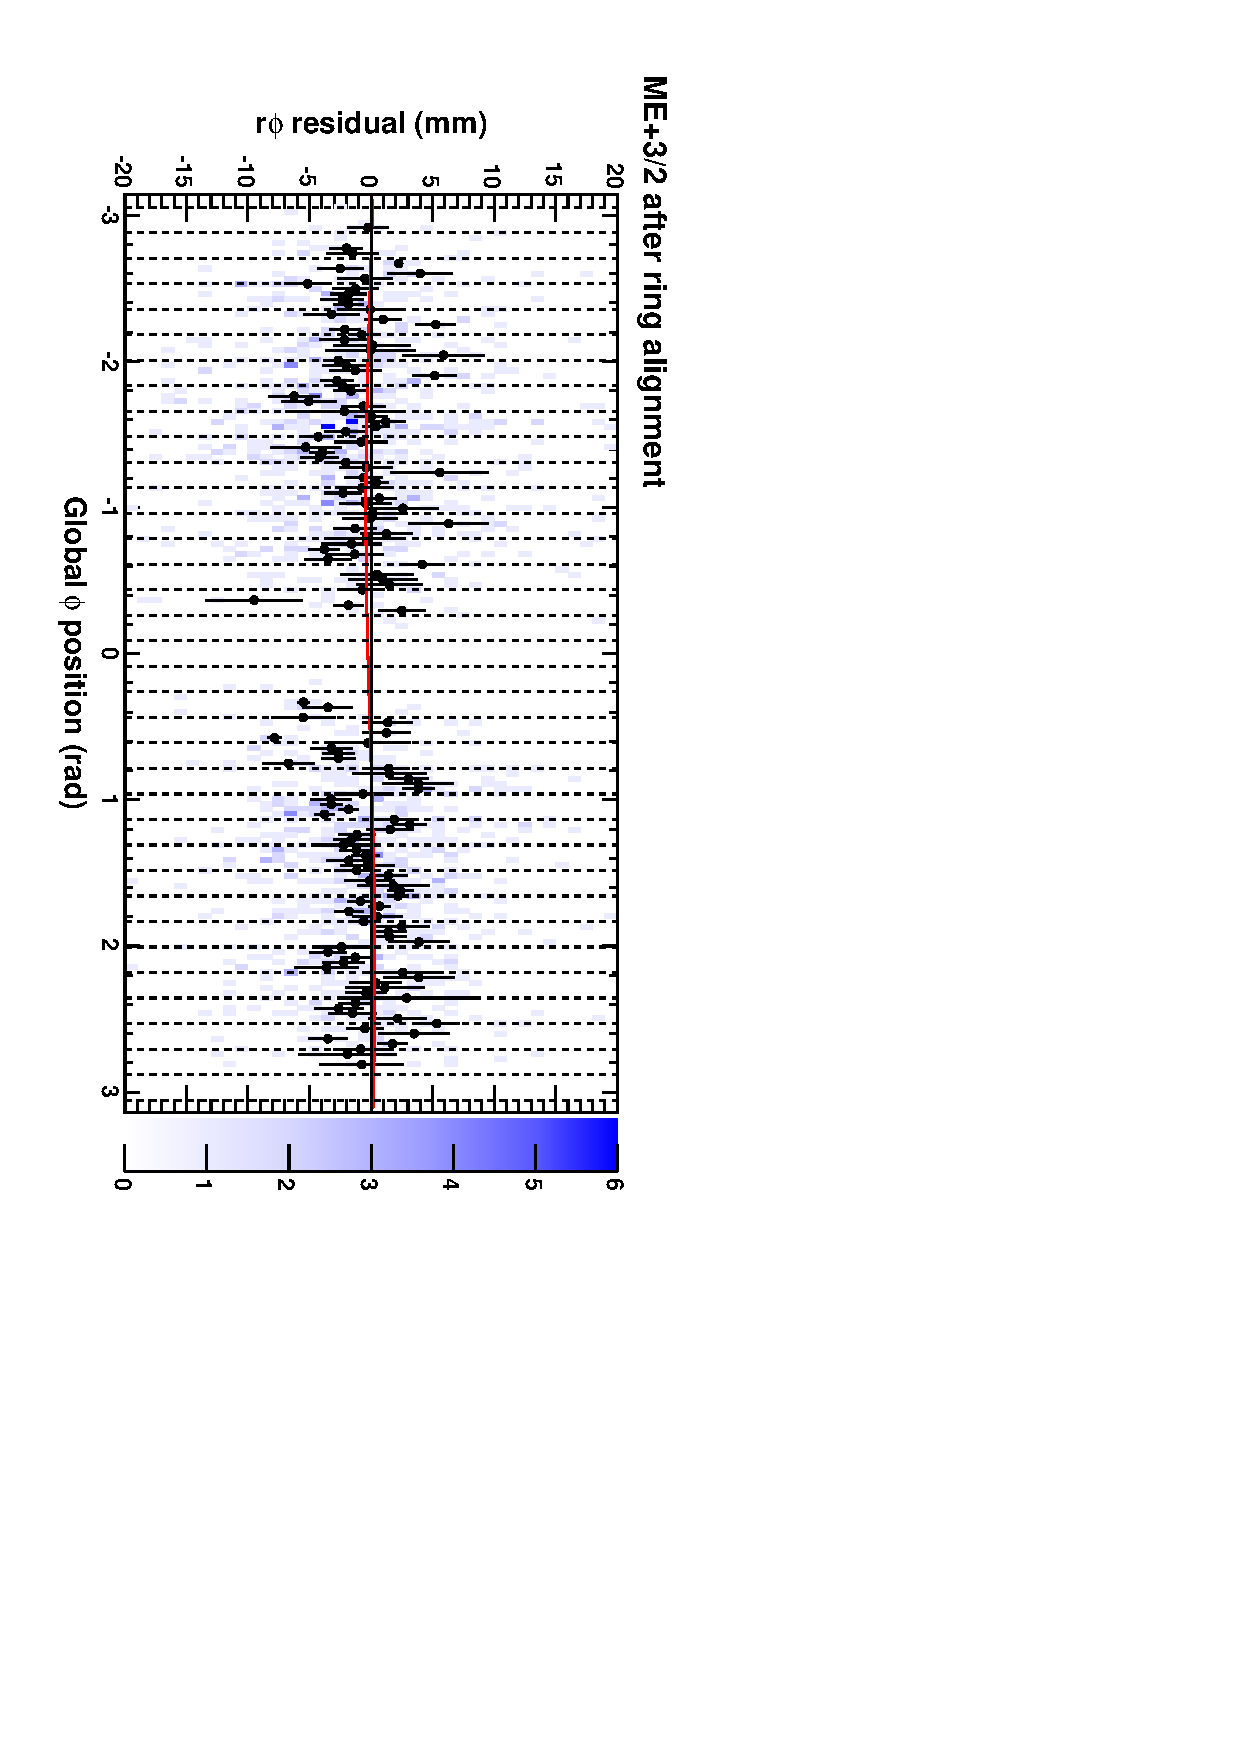
\includegraphics[height=\linewidth, angle=90]{ringfits_after/mep32.pdf}
\column{0.3\linewidth}
\begin{itemize}
\item Unbiased residuals from tracker tracks
\item Color scale is 2-D plot
\item Black points are a profile (averages in vertical bins)
\item Red line is fit to 2-D data
\item sine $\sim$ $X$ \\
cosine $\sim$ $Y$ \\
constant $\sim$ $\phi_Z$
\end{itemize}
\end{columns}
\end{frame}

\begin{frame}
\frametitle{Ring fits: ME$+$4/1}
\vfill
\begin{columns}
\column{0.7\linewidth}
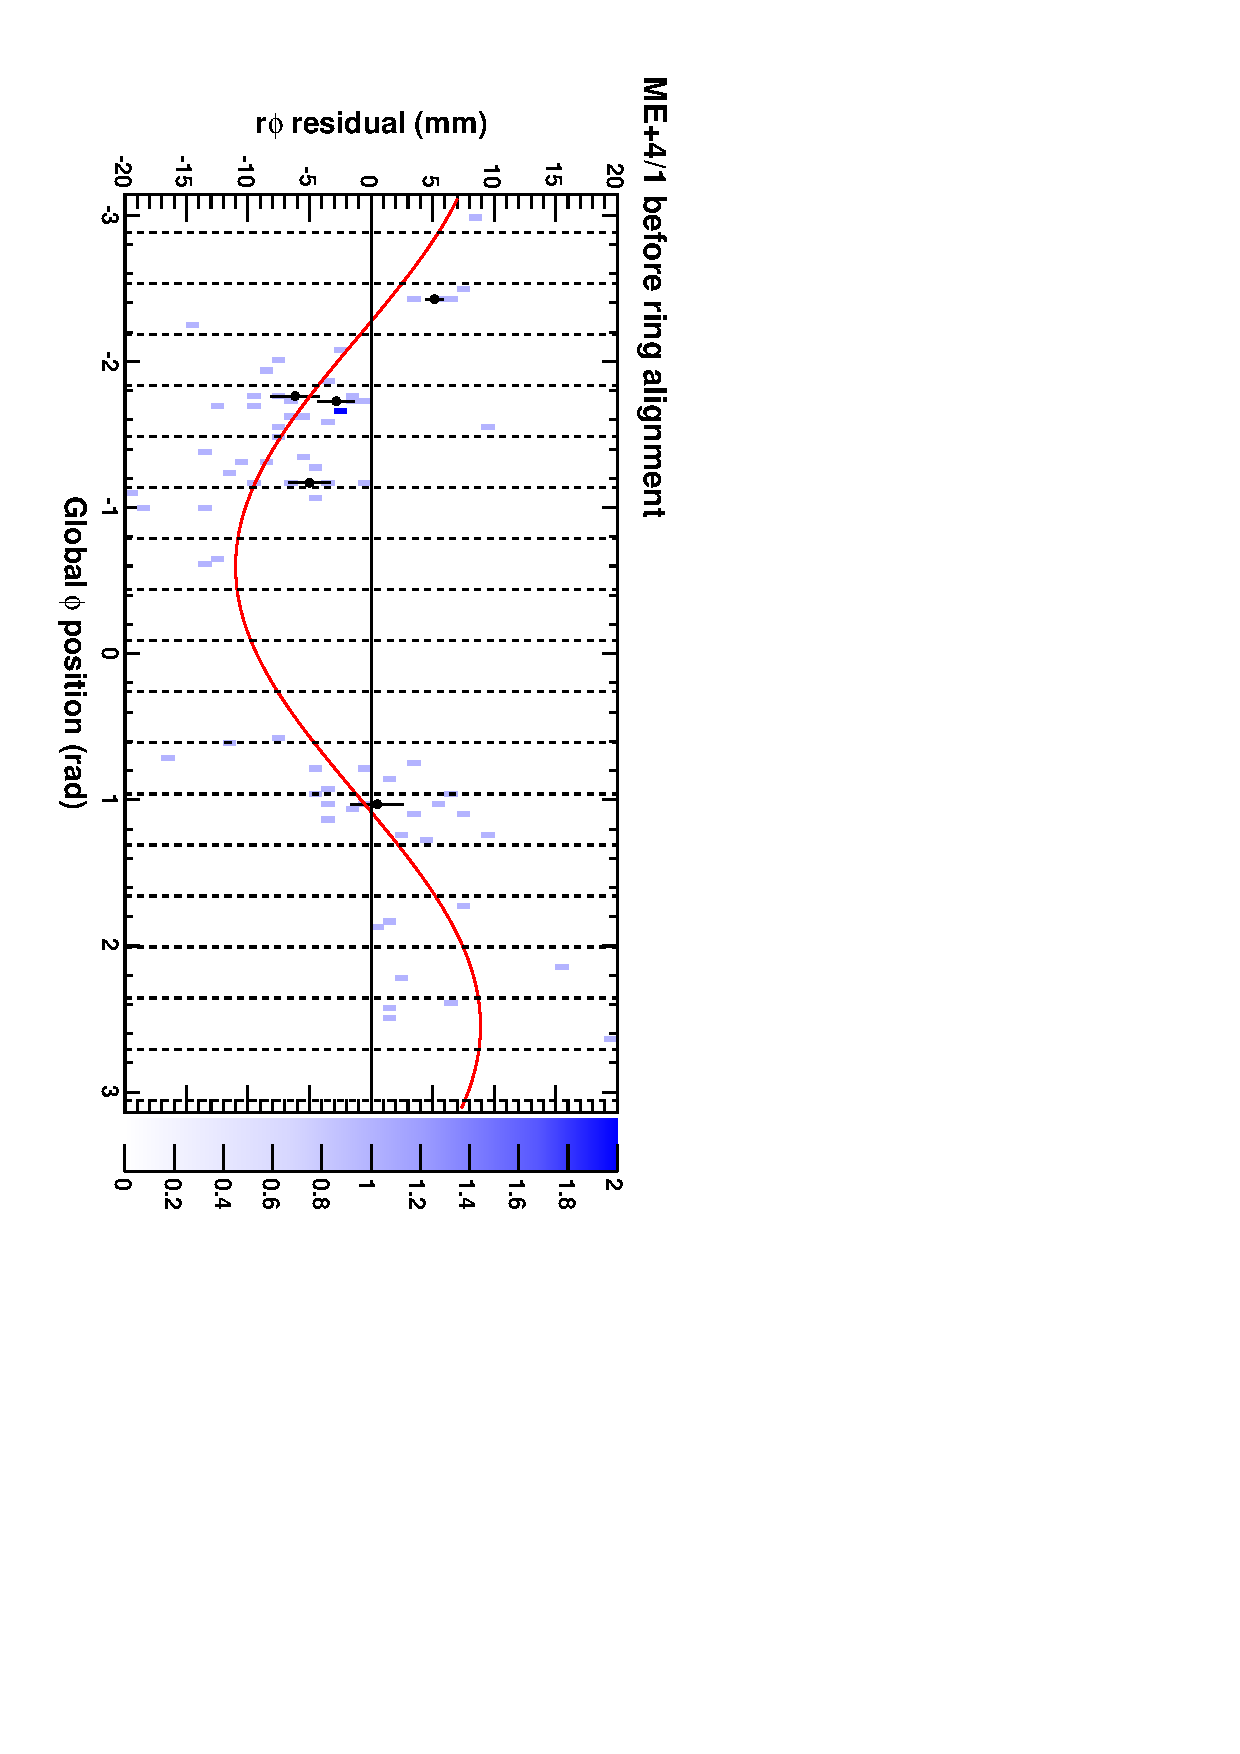
\includegraphics[height=\linewidth, angle=90]{ringfits_before/mep41.pdf}

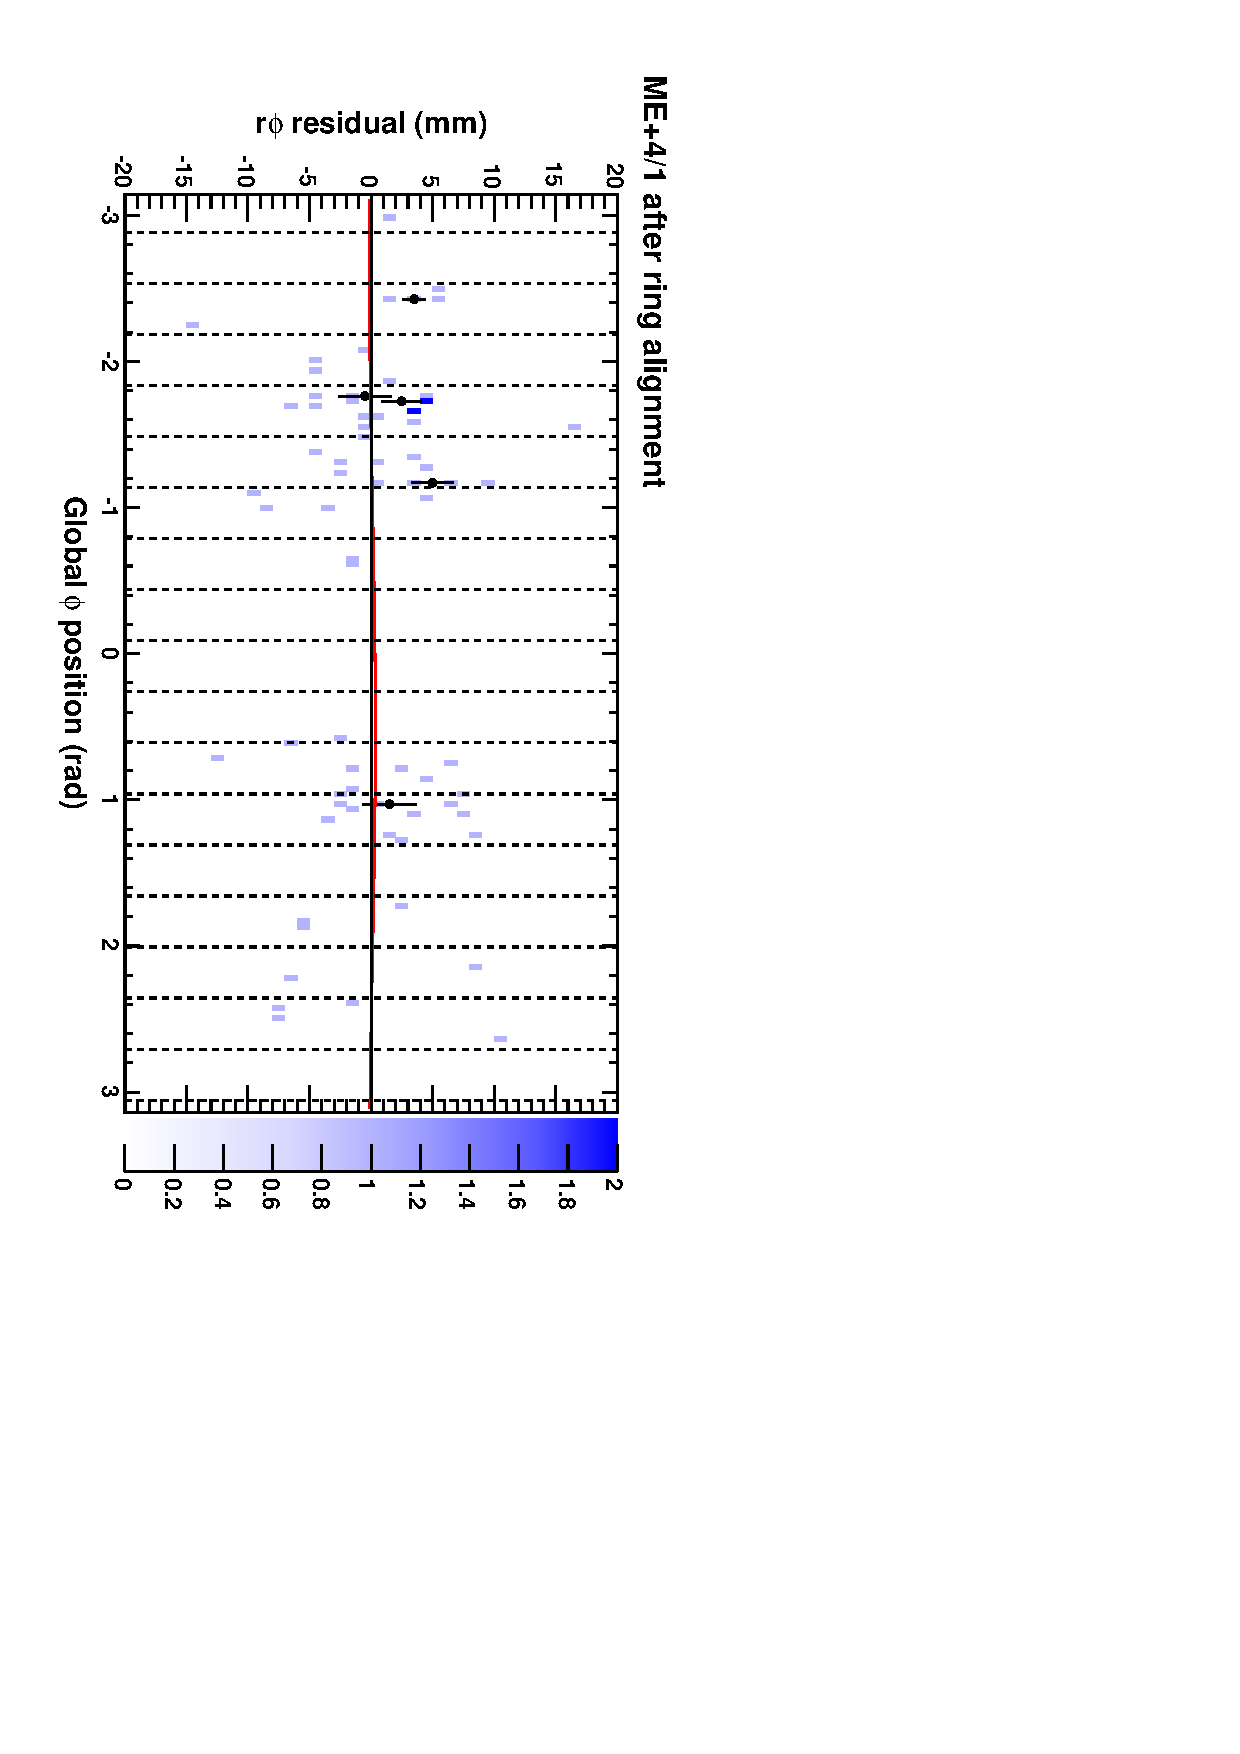
\includegraphics[height=\linewidth, angle=90]{ringfits_after/mep41.pdf}
\column{0.3\linewidth}
\begin{itemize}
\item Unbiased residuals from tracker tracks
\item Color scale is 2-D plot
\item Black points are a profile (averages in vertical bins)
\item Red line is fit to 2-D data
\item sine $\sim$ $X$ \\
cosine $\sim$ $Y$ \\
constant $\sim$ $\phi_Z$
\end{itemize}
\end{columns}
\end{frame}

\begin{frame}
\frametitle{Table of ring corrections}
\begin{itemize}
\item Grouped items are physically connected to the same disk; values are correlated but not exactly equal within fitting errors
\item Large $\chi^2/\mbox{ndf}$ expected from incomplete chamber alignment
\end{itemize}

\scriptsize
\renewcommand{\arraystretch}{1.1}
\begin{tabular}{c | c c c c}
ring & $\delta_x$ (mm) & $\delta_y$ (mm) & $\delta_{\phi_z}$ (mrad) & $\chi^2/\mbox{ndf}$ \\\hline
ME$-$4/1 & $ 5.00$ $\pm$ $ 0.14$ & $-1.30$ $\pm$ $ 0.22$ & $ 1.57$ $\pm$ $ 0.05$ & 79.8998 \\\hline
ME$-$3/2 & $ 2.25$ $\pm$ $ 0.04$ & $-0.62$ $\pm$ $ 0.06$ & $ 1.85$ $\pm$ $ 0.01$ & 60.1288 \\
ME$-$3/1 & $ 4.16$ $\pm$ $ 0.12$ & $ 0.06$ $\pm$ $ 0.18$ & $ 2.12$ $\pm$ $ 0.04$ & 63.914 \\
ME$-$2/2 & $ 1.66$ $\pm$ $ 0.04$ & $ 1.29$ $\pm$ $ 0.05$ & $ 1.68$ $\pm$ $ 0.01$ & 52.9565 \\
ME$-$2/1 & $ 3.77$ $\pm$ $ 0.09$ & $-1.96$ $\pm$ $ 0.13$ & $ 2.18$ $\pm$ $ 0.03$ & 37.8555 \\\hline
ME$-$1/3 & $ 2.41$ $\pm$ $ 0.06$ & $ 1.43$ $\pm$ $ 0.09$ & $ 0.26$ $\pm$ $ 0.01$ & 45.2275 \\
ME$-$1/2 & $ 3.52$ $\pm$ $ 0.05$ & $-1.56$ $\pm$ $ 0.07$ & $ 0.85$ $\pm$ $ 0.01$ & 23.7824 \\
ME$-$1/1 & $ 2.93$ $\pm$ $ 0.09$ & $-2.90$ $\pm$ $ 0.13$ & $ 0.66$ $\pm$ $ 0.04$ & 5.31818 \\\hline
ME$+$1/1 & $ 4.95$ $\pm$ $ 0.08$ & $-1.93$ $\pm$ $ 0.11$ & $ 0.17$ $\pm$ $ 0.04$ & 11.9906 \\
ME$+$1/2 & $ 5.05$ $\pm$ $ 0.05$ & $ 0.81$ $\pm$ $ 0.07$ & $ 0.13$ $\pm$ $ 0.01$ & 22.0969 \\
ME$+$1/3 & $ 4.36$ $\pm$ $ 0.06$ & $ 3.22$ $\pm$ $ 0.08$ & $ 0.02$ $\pm$ $ 0.01$ & 38.1421 \\\hline
ME$+$2/1 & $ 4.56$ $\pm$ $ 0.08$ & $ 2.30$ $\pm$ $ 0.12$ & $ 0.18$ $\pm$ $ 0.03$ & 28.5622 \\
ME$+$2/2 & $ 4.28$ $\pm$ $ 0.04$ & $ 3.86$ $\pm$ $ 0.05$ & $-0.11$ $\pm$ $ 0.01$ & 47.6725 \\
ME$+$3/1 & $ 5.06$ $\pm$ $ 0.10$ & $ 4.42$ $\pm$ $ 0.17$ & $-0.05$ $\pm$ $ 0.03$ & 25.2588 \\
ME$+$3/2 & $ 4.01$ $\pm$ $ 0.04$ & $ 4.88$ $\pm$ $ 0.06$ & $-0.37$ $\pm$ $ 0.01$ & 60.8494 \\\hline
ME$+$4/1 & $ 5.58$ $\pm$ $ 0.15$ & $ 8.24$ $\pm$ $ 0.24$ & $ 0.40$ $\pm$ $ 0.05$ & 31.3307 \\
\end{tabular}
\end{frame}

\begin{frame}
\frametitle{October Exercise (1)}
\begin{itemize}
\item Simulated alignment exercise with 3\_2\_X collisions/cosmics MC
\item Done in 2\_2\_X: \mbox{\tt \tiny https://hypernews.cern.ch/HyperNews/CMS/get/muon-alignment/342.html\hspace{-1 cm}}

\item Workflow performed by a new grad student, Aysen Tatarinov, from documentation and with help from Vadim Khotilovich and me

{\tt \tiny https://twiki.cern.ch/twiki//bin/view/CMS/SWGuideMuonAlignReferenceTarget}

\item Prelim.\ CSC resolution: 320~$\mu$m $\delta_x$, 290~$\mu$rad $\delta_{\phi_y}$, 590~$\mu$rad $\delta_{\phi_y}$

\mbox{\hspace{-1 cm} \scriptsize Note: I had encountered problems with ME1/3 in 2\_2\_X which appear to have been fixed!\hspace{-1 cm}}

\end{itemize}
\begin{center}
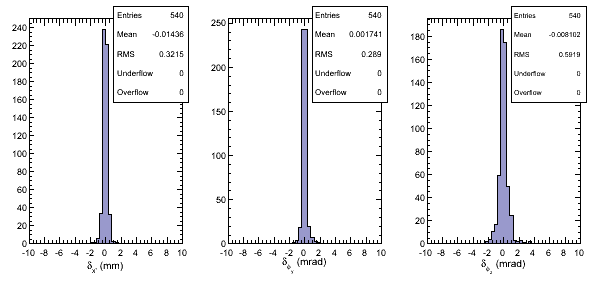
\includegraphics[width=0.9\linewidth]{only3_CSC.png}
\end{center}
\end{frame}

\begin{frame}
\frametitle{October Exercise (2)}
\begin{itemize}\setlength{\itemsep}{0.3 cm}
\item CSC Overlaps alignment was very successful in 2008 (2\_1\_X)
\item Software has not been updated since, might need small corrections to work in the new environment
\item Second October exercise: test CSC Overlaps in 3\_2\_X
\begin{itemize}
\item requested and recieved 3\_2\_X beam-halo sample
\item checked samples: everything is ready and in the right format
\item still need to work through exercise
\end{itemize}
\item Boundary condition: {\it real} beam-halo expected in $\sim$2
  weeks, algorithm must be fully vetted in Monte Carlo before then
\end{itemize}
\end{frame}

%% \begin{frame}
%% \frametitle{Outline}
%% \begin{itemize}\setlength{\itemsep}{0.75 cm}
%% \item 
%% \end{itemize}
%% %% \hspace{-0.83 cm} \textcolor{darkblue}{\Large Outline2}
%% \end{frame}

%% \section*{First section}
%% \begin{frame}
%% \begin{center}
%% \Huge \textcolor{blue}{First section}
%% \end{center}
%% \end{frame}

\begin{frame}
\frametitle{Summary}
\begin{itemize}\setlength{\itemsep}{0.75 cm}
\item Alternation feature strangely depends on $p_T$
\begin{itemize}
\item what could cause that?
\end{itemize}

\item CRAFT-09 alignment includes new corrections for large transverse disk displacement
\item Alignment machinery is being documented, has successfully been run by a new user
\item 2009 beam-halo is imminent: need to make sure tools are ready
\end{itemize}
\label{numpages}
\end{frame}

\end{document}
